\chapter{Úvod}

Mikrokontrolery (MCU) jsou monolitické integrované obvody obsahující mikroprocesor, paměť pro uložení programu, paměť pro jeho běh a další periferie
rozšiřující jeho funkčnost. Vyznačují se jednoduchostí, kompaktností a malou spotřebou. Používají se tak proto především pro jednoúčelová zařízení a 
vestavěné (embedded) systémy.

Při návrhu vestavěných systémů je v praxi často používána simulace. Díky využití simulátoru daného mikrokontroleru (případně celého vestavěného systému) lze ověřit funkčnost systému již při jeho návrhu aniž by bylo nutné vynaložit náklady na prvotní prototypy. Simulační čas lze zrychlit nebo naopak zpomalit a tím jednodušeji prozkoumat vybrané jevy. Simulace může rovněž zjednodušit hledání problémů viděných na reálném hardwaru, kdy jejich příčiny nelze prostým zkoumáním reálného systému jednoduše odhalit. Při použití simulace je také jednodušší vyzkoušet případné změny systému a zkoumat nové postupy bez dalšího zvýšení nákladů. Nejen z těchto důvodů je tedy simulace vestavěných systémů užitečná a má smysl se jí zabývat.

Tato diplomová práce si dává za cíl návrh a implementaci jednoduše rozšiřitelného pokročilého simulátoru mikrokontrolerů rodiny MSP430 od výrobce Texas Instruments. Tyto mikrokontrolery jsou hojně rozšířené především díky své nízké ceně, malé spotřebě a jednoduchosti práce s nimi. Lze je nalézt například i v platformě FITkit \cite{fitkit} používané k výukovým účelům Fakultou informačních technologií Vysokého učení technického v Brně. Simulátor implementovaný v této práci je navrhován právě jako doplňující prostředek pro vývoj aplikací pro tuto platformu, avšak bude moci být použit i samostatně. V současné době není obdobný software pod svobodnou licencí dostupný.

Tato diplomová práce je rozdělena do osmi kapitol.

První kapitola obsahuje úvod. Dále následuje kapitola stručně popisující strukturu mikrokontroleru MSP430, jeho instrukční sadu, základní interní periferie a formáty používané pro uložení binárního kódu tohoto mikrokontroleru. Třetí kapitola se zabývá událostně řízenou simulací, konkrétně pak formalismem DEVS. Ve čtvrté kapitole je proveden samotný návrh simulátoru. Popisem implementace tohoto návrhu se zabývá pátá kapitola. V šesté kapitole je implementovaný simulátor otestován porovnáním s reálným mikrokontrolerem MSP430. Sedmá kapitola popisuje formou případové studie možnosti rozšíření simulátoru o nové periferie. Na závěr je implementovaný simulátor zhodnocen.

\chapter{Mikrokontroler MSP430}

Tato kapitola stručně shrnuje základy architektury mikrokontrolerů rodiny MSP430. Nesnaží se však kompletně nahradit jejich dokumentaci \cite{msp430family} \cite{msp430book}, ačkoliv z ní vychází. Pro návrh a implementaci kompletního simulátoru nejsou informace v této kapitole dostačující, ale byly vybrány s ohledem na úvod do problematiky mikrokontrolerů MSP430 a pochopení následujících kapitol a činnosti navrhovaného simulátoru.

\begin{figure}[ht]
\centering
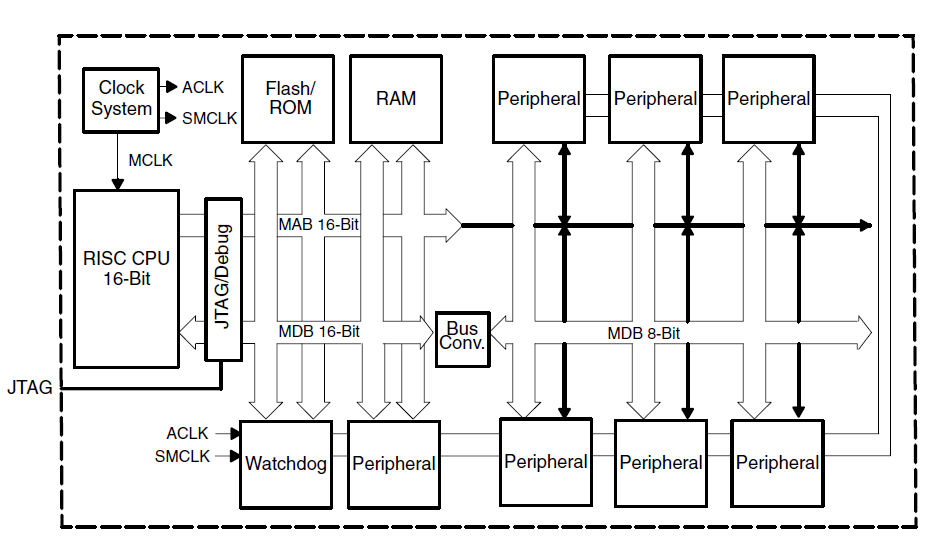
\includegraphics[trim=0cm 0cm 0cm 0cm, scale=0.5]{fig/msp430block}
\caption{Blokové schéma mikrokontroleru MSP430. Převzato z \cite{msp430family}.}
\label{fig:msp430block}
\end{figure}

Mikrokontroler je rozdělen na několik bloků, které lze vidět na obrázku \ref{fig:msp430block}. Jádrem celého mikrokontroleru je 16bitový mikroprocesor
vykonávající instrukce programu definované jeho instrukční sadou. Frekvence mikroprocesoru a všech dalších periferií je řízena systémem hodin (Clock System). K mikroprocesoru je pomocí 16bitové adresové sběrnice a 16bitové datové sběrnice připojena paměť programu (Flash/ROM) a paměť dat (RAM). Další doplňující periferie jsou pak adresovány adresovou sběrnicí o menší šířce v závislosti na modelu mikrokontroleru. Datová sběrnice periferií je buď 16bitová nebo 8bitová v závislosti na potřebě konkrétní periferie.

Jednotlivé bloky mikrokontroleru MSP430 jsou podrobněji popsány dále v této kapitole.

\section{Mikroprocesor a instrukční sada}

Mikrokontrolery rodiny MSP430 obsahují 16bitový mikroprocesor (CPU) a 16 registrů, každý o kapacitě 16 bitů. První čtyři registry mají speciální účel. Registr R0 slouží jako ukazatel na aktuální instrukci (PC - program counter). Register R1 ukazuje na vrchol zásobníku (SP - stack pointer). Register R2 je stavovým registrem (SR - status register) obsahující informace o stavu mikroprocesoru. Register R3 je použit pro generování často používaných konstant, takže je není potřeba načítat z paměti. Ostatní registry je možné volně využít v uživatelském programu.

Nejdůležitějšími stavovými bity ve stavovém registru jsou bity N (nastaven pokud je výsledek operace negativní), Z (nastaven pokud je výsledek operace nulový), C (nastaven pokud došlo k přenosu nejvyššího bitu) a V (nastaven pokud došlo při operaci k přetečení).

\subsection{Instrukční sada}

Instrukční sada obsahuje 27 instrukcí. Instrukce jsou kódovány pomocí 16, 32 nebo 48 bitů přičemž operační kód je situován vždy v prvních 16 bitech.

Většina instrukcí pracujících s daty umí pracovat jak s operandem velikosti jednoho bytu, tak s celým slovem. Instrukce lze rozdělit do 3 typů, které se liší i rozdílným kódováním v prvních 16 bitech instrukce uložené v paměti:

\subsubsection{Instrukce s jedním operandem}

V závislosti na operačním kódu (opcode) rozlišuje mikroprocesor následující jednooperandové instrukce (.B značí bytovou formu instrukce):

\begin{itemize}
\item \textbf{RRC(.B)} - 9 bitová rotace s přenosem nejvyššího bitu.
\item \textbf{SWPB} - Záměna horních a spodních 8 bitů v rámci jednoho registru.
\item \textbf{RRA(.B)} - 8 bitový aritmetický posun doprava.
\item \textbf{SXT} - Rozšíření znaménka z 8 bitů na 16 bitů.
\item \textbf{PUSH(.B)} - Uložení operandu na zásobník. Sníží hodnotu SP o 2.
\item \textbf{CALL} - Volání podprogramu. Získá operand, uloží PC na zásobník a do PC uloží hodnotu operandu.
\item \textbf{RETI} - Návrat z přerušení. Obnoví ze zásobníku SP a PC.
\end{itemize}

\subsubsection{Instrukce s dvěma operandy}

Mikrokontroler MSP430 rozlišuje tyto instrukce se dvěma operandy a provádí s nimi následující operace:

\begin{itemize}
\item \textbf{MOV src,dest} - dest = src
\item \textbf{ADD src,dest} - dest += src
\item \textbf{ADDC src,dest} - dest += src + C
\item \textbf{SUBC src,dest} - dest += ~src + C
\item \textbf{SUB src,dest} - dest -= src
\item \textbf{CMP src,dest} - dest - src (Mění pouze stavový registr)
\item \textbf{DADD src,dest} - dest += src + C, BCD.
\item \textbf{BIT src,dest} - dest \& src (Mění pouze stavový registr)
\item \textbf{BIC src,dest} - dest \&= ~src
\item \textbf{BIS src,dest} - dest |= src
\item \textbf{XOR src,dest} - dest \^ = src
\item \textbf{AND src,dest} - dest \&=- src
\end{itemize}

\subsubsection{Podmíněné instrukce}

Podmíněné instrukce jsou typicky instrukce skoků, které provedou skok pouze při splnění určité podmínky (hodnoty konkrétního bitu ze stavového registru). Zpravidla je před nimi volání instrukce CMP pro porovnání dvou hodnot a nastavení stavového registru. Opět je rozlišeno několik druhů podmíněných instrukcí:

\begin{itemize}
\item \textbf{JNE/JNZ} - Provede skok pokud Z==0 (po zavolání CMP se 2 hodnoty nerovnají).
\item \textbf{JEQ/Z} - Provede skok pokud Z==1 (po zavolání CMP se 2 hodnoty rovnají).
\item \textbf{JNC/JLO} - Provede skok pokud C==0 (po zavolání CMP je první neznaménková hodnota menší než druhá).
\item \textbf{JC/JHS} - Provede skok pokud C==1 (po zavolání CMP je první neznaménková hodnota vetší nebo rovna druhé).
\item \textbf{JN} - Provede skok pokud N==1.
\item \textbf{JGE} - Provede skok pokud N==V (po zavolání CMP je první znaménková hodnota vetší nebo rovna druhé).
\item \textbf{JL} - Provede skok pokud N!=V (po zavolání CMP je první znaménková hodnota menší než druhá).
\item \textbf{JMP} - Provede skok vždy.
\end{itemize}

\subsubsection{Časování instrukcí}

Každá instrukce potřebuje ke svému vykonání určitý počet hodinových cyklů. Zpravidla je zapotřebí 1 cyklus pro každý přístup do paměti. Z tohoto pravidla však existuje několik výjimek popsaných v dokumentaci k mikrokontrolerům MSP430.
 
\subsection{Adresové módy}

Mikrokontroler MSP430 pracuje se 7 adresovými módy pro zdrojový operand a 4 adresovými módy (první 4 módy následujícího seznamu) pro operand cílový:

\begin{itemize}
\item \textbf{Registrový mód} - Rn - Operand je uložen v registru Rn.
\item \textbf{Indexový mód} - X(Rn) - Operand je uložen v paměti na adrese Rn + X. X je uloženo v následujícím slově za instrukcí.
\item \textbf{Symbolický mód} - ADDR - Operand je uložen v paměti na adrese PC + X. X je uloženo v následujícím slově za instrukcí.
\item \textbf{Absolutní mód} - \&ADDR - Adresa operandu je uložena v následujícím slově za instrukcí.
\item \textbf{Nepřímý registrový mód} - @Rn - Register Rn ukažuje na umístění operandu.
\item \textbf{Nepřímý mód s automatickou inkrementací} - Register Rn ukazuje na umístění operandu. Rn je inkrementován o hodnotu 1 (přístup k bytu) nebo o 2 (přístup ke slovu).
\item \textbf{Immediate mód} - Hodnota operandu je umístěna v následujícím slově za instrukcí.
\end{itemize}

\subsection{Přerušení}

Přerušení umožňují přerušit běh uživatelského programu při určité události. Po příchodu přerušení je vyvolána rutina obsluhující přerušení na základě její adresy ve vektoru přerušení. Po obsloužení přerušení mikroprocesor pokračuje dále ve vykonávaní uživatelského programu.

Přerušení mají své pevně dané priority. Pokud dojde k více žádostem o přerušení, je přednostně obsloužena žádost s vyšší prioritou.

\section{Základní hodinový modul}

Jednou z dílčích částí mikrokontrolerů rodiny MSP430 je základní hodinový modul (Basic Clock Module/Clock System). Poskytuje hodinový signál pro mikroprocesor a periferie mikrokontroleru. Ve většině variant mikrokontroleru MSP430 jsou v rámci hodinového modulu implementovány 4 možné zdroje hodin:

\begin{itemize}
\item \textbf{LFXT1CLK} - Nízko-frekvenční/vysoko-frekvenční oscilátor, který může být použit s externím krystalem, rezonátorem nebo vstupem externího hodinového signálu (typicky o frekcenci 32768 Hz).
\item \textbf{XT2CLK} - Oscilátor, který může být použit s externím krystalem, rezonátorem nebo vstupem externího hodinového signálu o frekvenci 400 kHz až 16 Mhz.
\item \textbf{DCOCLK} - Digitálně kontrolovaný oscilátor. Jeho frekvenci lze nastavit pomocí registrů (například u MSP430G2253 od 1 Mhz do 16 Mhz).
\item \textbf{VLOCLK} - Interní nízkofrekvenční oscilátor s typickou frekcení 12 kHz.
\end{itemize}

Tyto zdroje hodin lze pak použít jako vstup ve 3 zdrojích hodinového signálu:

\begin{itemize}
\item \textbf{MCLK} - Hlavní hodiny (Master clock) určují frekcenci běhu CPU.
\item \textbf{SMCLK} - Vedlejší hodiny (Sub-main clock) určují frekcenci ostatních periferií.
\item \textbf{ACLK} - Pomocné hodiny (Auxiliary clock). Jako zdroj může být použit pouze LFXT1CLK nebo VLOCLK.
\end{itemize}

\section{Základní periferie}

Mikrokontrolery MSP430 obsahují velké množství periferií jako jsou například časovače, moduly pro digitální vstup a výstup, AD převodník nebo komunikační moduly. Každá periferie má vlastní registry přístupné na předem dané paměťové adrese, které slouží k jejímu řízení. V rámci této podkapitoly jsou zmíněny a stručně popsány nejpoužívanější periferie.

\subsection{Digitální vstup a výstup}

Základní činností mikrokontroleru je jeho komunikace s okolím. Mikrokontroler MSP430 obsahuje několik vstupně/výstupních portů (P1 až Px), kde každý port obsahuje 8 pinů. Jednotlivé piny mohou být nastaveny jako vstupní respektive výstupní a lze číst jejich logickou hodnotu respektive ji zapisovat. Některé z portů podporují generování přerušení při změně logické úrovně na pinech.

Pro ovládání digitálního vstupu a výstupu jednotlivých portů jsou k dispozici následující registry mapované do paměti RAM:

\begin{itemize}
\item \textbf{PxIN} - Hodnoty bitů určují aktuální logickou hodnotu na pinu (v případě že je pin nastaven jako vstupní).
\item \textbf{PxOUT} - Jednotlivé bity nastavují výstupní logickou hodnotu na pinu.
\item \textbf{PxDIR} - Logická 0 na daném bitu nastavuje pin jako vstupní. V opačném případě je pin výstupní.
\end{itemize}

K pinům mohou být připojeny i další periferie jako například časovač nebo AD převodník. Aby bylo možné určit, která periferie bude na daném pinu aktivní, jsou po každý port k dispozici další dva registry PxSEL a PxSEL2. Kombinace 2 bitů pro každý pin v těchto registrech pak určuje konkrétní periferii, která
bude k pinu interně připojena a bude jej obsluhovat.

\subsection{Časovač}

Časovač je ve své podstatě 16bitový čítač, který mění svou hodnotu s každým tikem hodin (SMCLK nebo ACLK). Mikrokontrolery MSP430 obsahují 2 samostatné moduly časovače: Timer A a Timer B. V této podkapitole jsou popsány pouze vlastnosti shodné pro oba časovače.

Hodnota časovače se mění v závislosti na zvoleném módu:
\begin{itemize}
\item \textbf{Up mode} - Časovač opakovaně počítá od nuly po hodnotu v registru TACCR0.
\item \textbf{Continuous mode} - Časovač opakovaně počítá od nuly po hodnotu 0xffff.
\item \textbf{Up/Down mode} - Časovač opakovaně počítá od nuly po hodnotu v registru TACCR0 a pak zpět do nuly.
\end{itemize}

\subsubsection{Capture/Compare bloky}

Časovač se skládá z více samostatných Capture/Compare bloků. Každý z těchto bloků umožňuje pracovat ve dvou módech.

Prvním módem je Capture mód. Časovač je v tomto módu připojen k externímu pinu. Pokud na pinu dojde ke změně logické hodnoty, dojde ke zkopírování aktuální hodnoty časovače do CCR registru a je vyvoláno přerušení. Lze tak například zjistit délku pulzu na vstupu.

Pokud je Capture/Compare blok v Compare módu a hodnota časovače je rovna hodnotě CCR registru, je vygenerováno přerušení a na externí pin lze podle nastavení generovat výstup. Compare mód je využíván pro generování PWM signálu nebo pro generování pravidelných přerušení.

\subsection{Komunikační moduly}

Mikrokontrolery MSP430 obsahují v závislosti na modelu různé komunikační moduly. Komunikační moduly umožňují hardwarovou komunikaci mikrokontroleru s jiným zařízením pomocí předem stanoveného protokolu a přenosové rychlosti. Tato podkapitola stručně shrnuje možné komunikační moduly a protokol SPI. Jednotlivé moduly podporují i jiné protokoly, ale v rámci této diplomové práce byla implementována pouze komunikace za použití protokolu SPI.

\subsubsection{Protokol SPI}

Protokol SPI (Serial Peripheral Interface) definuje komunikaci mezi zařízeními propojenými třemi vodiči z nichž jedno ze zařízení je master a ostatní jsou slave. Jedná se o vodič SCLK přenášející hodinový signál určující frekvenci komunikace (generuje master), vodič SDO přenášející data ze zařízení a vodič SDI přenášející data do zařízení.

Existuje i možnost komunikace pomocí 4 vodičů. Čtvrtým vodičem je v tomto případě vodič STE zajišťující vybrání konkrétního slave zařízení, které bude data spracovávat.

Samotná komunikace pak probíhá tak, že se s každým tikem hodin přenese po vodičích SDO a SDI jeden bit, zařízení jej přečtou a uloží do paměti. Takto se přenese všech N bitů.

\subsubsection{Komunikační modul USI}

Komunikační modul USI (Universal Seria Interface) poskytuje synchronní sériovou komunikaci. Jeho základem je 8bitový nebo 16bitový posuvný registr, ze kterého jsou postupně vybírány výstupní bity a vstupní bity jsou do něj nahrávány. Modul USI podporuje přerušení, takže jeho běh nevyžaduje ze strany softwaru nadbytečné řízení.

Lze zvolit mezi přenosem 8 nebo 16 bitů a jejich orientací - MSB nebo LSB. Lze rovněž nastavit fázi a polaritu hodin generovaného signálu. Jako vstup hodinového signálu lze zvolit ACLK, SMCLK, SCLK (externí hodinový signál), výstup z časovače nebo jej ovládat softwarově zápisem do registru.

Tento komunikační modul je implementován ve starších modelech mikrokontroleru MSP430. V novějších jej nahradil modul USCI.

\subsubsection{Komunikační modul USCI}

Modul USCI (Universal Serial Communication Interface) podporuje více komunikačních protokolů (SPI, I2C, UART) v rámci jediného modulu. USCI modul je interně tvořen sadou podmodulů, které poskytují specifické komunikační protokoly.

V případě protokolu SPI lze zvolit mezi přenosem sedmi nebo osmi bitů a lze určit jejich pořadí - MSB nebo LSB. Narozdíl od modulu USI podporuje modul USCI i komunikaci pomocí 4 vodičů. Registry pro přijatá a odeslaná data jsou od sebe odděleny a ke každému z nich existuje buffer, čímž je umožněna nepřerušená komunikace.

Lze taktéž zvolit polaritu a fázi generovaného hodinového signálu a jako jeho vstup využít ACLK neb SMCLK.

\subsubsection{Komunikační modul USART}

Komunikační modul USART (Universal Synchronous/Asynchronous Receive/Transmit) podporuje 2 komunikační protokoly - SPI a UART. Z hlediska funkčnosti se jeho vlastnosti pro protokol SPI neliší od modulu USCI, liší se pouze vnitřní architekturou a rozdílným řízením ze strany software.


\section{Formáty uložení spustitelného kódu}

Tato podkapitola shrnuje dva nejpoužívanější formáty pro uložení binárního kódu, který je nahráván do mikrokontrolerů. Jedná se o formáty Intel HEX (A43) a ELF. Je důležité se s nimi seznámit, protože je navrhovaný simulátor bude muset načítat a zpracovávat.

\subsection{Intel HEX (A43)}

Jedná se o jednoduchý textový formát obsahující jednotlivé byty programu, jejich umístění v paměti a adresu začátku programu. Formát byl specifikován roku 1988 firmou Intel \cite{intelhex}. Na obrázku \ref{fig:intelhex} lze vidět okomentovanou ukázku formátu Intel HEX.

\begin{figure}[ht]
\centering
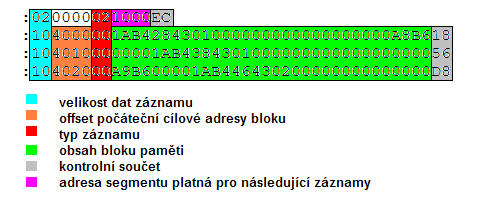
\includegraphics[trim=0cm 0cm 0cm 0cm, scale=0.7]{fig/intelhex}
\caption{Ukázka souboru ve formátu Intel HEX s popisky. Převzato z \cite{intelhex2}.}
\label{fig:intelhex}
\end{figure}

Formát Intel HEX pro MSP430 používá následující 4 typy záznamu:

\begin{itemize}
\item \textbf{00} - Datový záznam obsahující samotná data a 16bitovou adresu dat.
\item \textbf{01} - Konec souboru.
\item \textbf{02} - Rozšiřující segmentový záznam (MSB). Je používán pouze v případě, kdy je potřeba adresovat více než 16 bity.
\item \textbf{03} - Startovací záznam určující prvotní hodnotu PC registru (adresa daná jako segment (16 bitů) a offset (16 bitů); nejprve MSB)
\end{itemize}

\subsection{ELF}

Formát ELF (Executable and Linkable Format) je komplexní formát pro ukládání spustitelných souborů. Je rozšířen převážně na Unixových systémech. Formát ELF je základním výstupním formátem překladače GCC, který je často používán pro kompilování programů pro mikrokontroler MSP430. Kolem překladače GCC existuje řada dalších nástrojů, které umožňují získat z ELF souboru další informace aniž by musel programátor implementovat parser formátu ELF. \cite{elf}

Jedním z těchto nástrojů je program objcopy umožňující převod z ELF formátu do jiných formátů. Lze jím převést soubor z formátu ELF do formátu Intel HEX, který lze snadněji zpracovat. Dalším nástrojem je nástroj objdump. Pomocí tohoto nástroje lze například disassemblovat program obsažený v ELF souboru.

\subsubsection{DWARF - ladící informace}

Klíčovou vlastností formátu ELF je však možnost uložení ladících informací ve formátu DWARF. Popis DWARF formátu v této podkapitole vychází z \cite{dwarf}. Jedná se v podstatě o strom reprezentující celý výsledný
program. Jednotlivé části programu (zdrojové soubory, funkce, globální a lokální proměnné, datové typy atd.) jsou uzly tohoto stromu. Debuggery (jako je například GDB) pak těchto informací využívají při ladění programu a umožňují zobrazovat detailní ladící informace jako je hodnota lokální proměnné nebo zdrojový kód dané funkce.

\begin{figure}[ht]
\centering
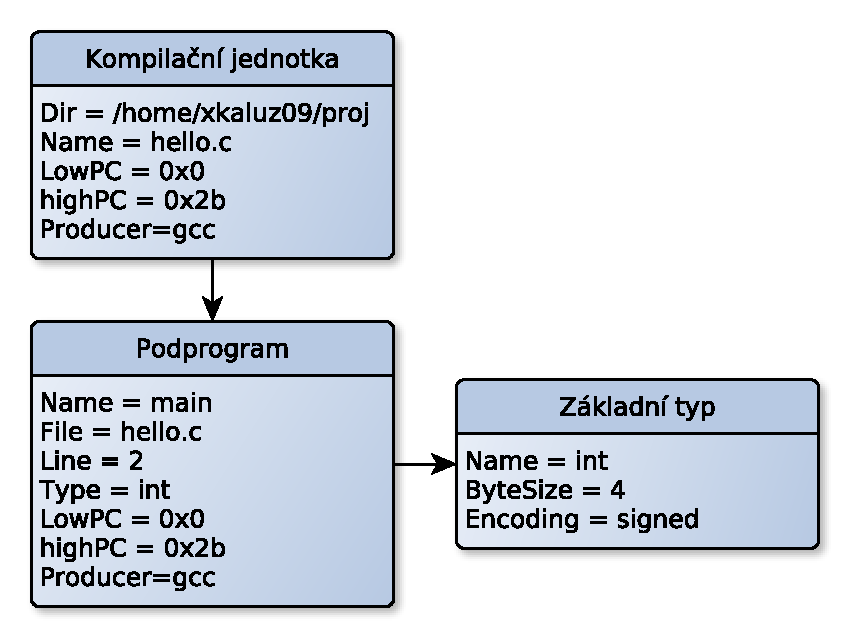
\includegraphics[trim=0cm 0cm 0cm 0cm, scale=0.7]{fig/dwarf}
\caption{DWARF strom Hello World programu v jazyce C.}
\label{fig:dwarf}
\end{figure}

Na obrázku \ref{fig:dwarf} lze vidět DWARF strom vygenerovaný pro jednoduchý program typu Hello World v jazyce C. Ze stromu je patrné, že každý uzel má svůj typ, od kterého se odvíjí jeho další atributy. Kořenem stromu je kompilační jednotka "hello.c" s atributy lowPC a highPC. Kdykoliv se vykonávání programu zastaví na instrukci s adresou mezi těmito dvěma atributy, jedná se o instrukci generovanou z této kompilační jednotky. V rámci této kompilační jednotky je definován pouze jediný podprogram "main" s návratovou hodnotou typu "int". Pokud by bylo podprogramů více, lze opět konkrétní podprogram určit za pomocí atributů lowPC a highPC a adresy aktuální instrukce. Datový typ "int" je definován jako základní znaménkový typ s velikostí 4 byty.

Formát DWARF definuje velké množství typů uzlů a jejich atributů. Z hlediska simulátorů je však důležité popsat ještě uložení proměnných. Proměnné mají kromě svého jména a typu ještě lokaci. Ta definuje, kde se nachází hodnota proměnné. Adresa proměnné se však může během běhu programu měnit - někdy bude výhodné mít proměnnou v registru, jindy v paměti, nebo dokonce z části v registru a z části v paměti. Proto je lokace proměnné ve formátu DWARF většinou definována v závislosti na adrese aktuální instrukce v takzvaném seznamu lokací.

Seznam lokací obsahuje pro každou proměnnou její lokaci v závislosti na adrese aktuální instrukce. Každá lokace je pak tvořena kódem zásobníkového automatu se speciálními mikroinstrukcemi, po jehož vykonání je na jeho vrcholu buď samotná hodnota proměnné, číslo registru ve kterém se hodnota nachází nebo
adresa místa v paměti, kde hodnotu najdeme.

K získání těchto informací z ELF souboru lze opět použít nástroj objdump.

\chapter{Událostně řízená simulace}

Udáje v této kapitole popisující událostně řízenou simulaci vychází z \cite{nutaro}.

Událostně řízená simulace modeluje simulovaný systém jako sled diskrétních událostí. Každá událost se odehrává v přesně stanoveném čase a mění celkový
stav systému. Mezi jednotlivými událostmi se stav systému nemění a je tak možné zpracovávat po sobě jdoucí události bez ohledu na časový interval
mezi nimi.

Kromě událostně řízené simulace existuje také simulace spojitá. Tento typ simulace probíhá tak, že je simulační čas rozdělen na malé časové intervaly, ve kterých se pak počítá celkový stav systému. Oproti událostně řízené simulaci je spojitá simulace mnohonásobně pomalejší než ekvivalentní událostně řízená simulace.

\subsubsection{Příklad událostně řízené simulace}

Další podkapitoly v této kapitole se budou odkazovat na následující typický příklad událostně řízené simulace - Frontu v obchodním domě (viz obrázek \ref{fig:bank}).

\begin{figure}[ht]
\centering
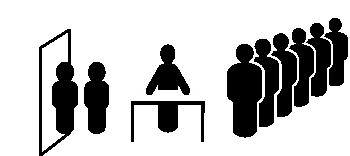
\includegraphics[trim=0cm 0cm 0cm 0cm]{fig/bank}
\caption{Ilustrace modelového příklady fronty v obchodním domě. Převzato z \cite{adevs}.}
\label{fig:bank}
\end{figure}

Zákaznící mohou přicházet do obchodu a jsou obslouženi pokladní v pořadí, v jakém k pokladně přisli. Čas potřebný k odbavení zákazníka je závislý na počtu položek v jeho nákupním koši (Takže je pro každého zákazníka rozdílný).

První entitou takovéto simulace je Zákazník. O každém zákazníkovi potřebujeme vědět dobu, za jakou ho pokladník odbaví, čas příchodu do fronty a čas jeho odbavení (abychom byli schopni zjistit dobu jakou zákazník ve frontě strávil).

Další entitou simulace je Pokladní. Pokladní má před sebou frontu čekajících zákazníků, které musí obsloužit. Pokud pokladní neobsluhuje zákazníka a fronta není prázdná, začne prvního zákazníka ve frontě obsluhovat. Obsloužený zákazník je odebrán z fronty. V případě kdy ve frontě není žádný zákazník, pokladní nic nedělá.

Cílem simulace bude zjištění průměrného času stráveného zákazníkem ve frontě.

\section{Komponenty událostně řízené simulace}

Abychom mohli příklad z úvodu této kapitoly simulovat, je potřeba definovat základní komponenty událostně řízené simulace. Vysvětlení následujících termínů vychází z \cite{dess}.

\subsubsection{Entita}

Entitou rozumíme jakýkoliv objekt zájmu v systému. V příkladu obchodního domu se jedná například o pokladníka nebo zákazníka. Každá entita může mít své atributy - vlastnosti.

\subsubsection{Stav systému}

Každá událostně řízená simulace má svůj globální stav systému. Ten zahrnuje všechny proměnné a atributy studovaného systému. Globální stav se může v průběhu
simulace měnit vykonáváním událostí.

\subsubsection{Čas}

Simulace musí udržovat svůj simulační čas. Jednotky času nejsou pevně definovány a jejich volba je na vývojáři. Jak již bylo zmíněno, simulační čas se nemění spojitě, ale mění se skokově s jednotlivými událostmi.

\subsubsection{Seznam událostí}

Další důležitou částí událostně řízené simulace je seznam událostí. V seznamu jsou události, které ještě nebyly zpracovány. O každé události je znám čas, ve kterém se má udát, a kód potřebný k jejímu vykonání. Události jsou seřazeny vzestupně podle simulačního času. Pokud je simulace jednovláknová, existuje vždy právě jedna aktuálně prováděná událost.

Události jsou vetšinou do seznamu událostí přidávány dynamicky v průběhu simulace. V příkladu obchodního domu je například po startu simulace na čas $t$ naplánována událost příchodu nového zákazníka do fronty. Pokud v tu dobu nebyl ve frontě žádný zákazník, může být rovnou naplánována i událost odbavení tohoto zákazníka na čas $t+s$, kde $s$ je doba obsluhy zákazníka pokladním.

\subsubsection{Generátor náhodných čísel}

Simulace využívá náhodných čísel například pro generování časů událostí. V příkladu s obchodním domem jde například o generování příchozích zákazníků řadících se na konec fronty. Většinou jsou využity pseudo-náhodné generátory. Umožňují totiž opakovat simulaci se stejným průběhem.

\subsubsection{Statistiky}

V průběhu simulace se obvykle udržují statistiky o běhu systému. Jedná se o různé informace, které jsou z hlediska simulace zajímavé. Pro obchodní dům může jít například o průměrnou dobu čekání zákazníka ve frontě.

\subsubsection{Ukončovací podmínka}

Protože události jsou generovány dynamicky v průběhu simulace, mohla by být simulace nekonečná. Je tak potřeba definovat podmínku pro její ukončení. Typicky je simulace ukončena po dosažení určitého simulačního času, nebo například po zpracování určitého počtu událostí (například po určitém počtu obsloužených zákazníků).

\section{Průběh událostně řízené simulace}

Událostně řízená simulace se obecně řídí následujícím algoritmem:

\begin{itemize}
\item Inicializace stavu systému a ukončovací podmínky na False. 
\item Inicializace hodin (obvykle na hodnotu 0).
\item Naplánování prvotní události (její vložení do seznamu událostí).
\item Dokud není ukončovací podmínka rovna True:
\begin{itemize}
\item Nastavení hodin na čas další události podle seznamu událostí.
\item Vykonání události a její odstranění ze seznamu událostí.
\item Aktualizace statistik systému.
\end{itemize}
\item Vygenerování hlášení o simulaci.
\end{itemize}

\section{Formalismus DEVS pro modelování systémů}

DEVS (Discrete Event System Specification) je hierarchický a modulární formalismus pro návrh a modelování systémů s diskrétními událostmi. Jeho autorem je profesor Bernard P. Zeigler, který jej poprvé publikoval ve své knize Theory of Modeling and Simulation \cite{zeigler}. Právě modularita tohoto přístupu k událostně řízené simulaci jej dělá optimální pro tvorbu modulárního simulátoru.

DEVS definuje jak strukturu tak chování systému. Chování jednotlivých entit systému je popsáno pomocí atomického modelu. Struktura celého systému (tzv. propojení jednotlivých atomických modelů) popisuje spojovaný model. Tato podkapitola stručně popisuje tyto dva modely.

\subsection{Atomický model}

Základem formalismu DEVS je atomický model popisující chování části systému. Atomický model modeluje dynamický systém, který se mění v důsledku změny jeho okolí a své okolí ovlivňuje svými změnami.

Proměnné, které mění atomický model označujeme jako jeho vstupy a popisujeme jako množinu $X$. Jako $Y$ označujeme množinu výstupů modelu, které pak mění jeho okolí. Množina atributů, které definují interní stav atomického modelu značíme jako $S$.

Chování atomického modelu je definováno jeho přechodovými funkcemi (interní a externí), jeho výstupní funkcí a funkcí posunu času.

\subsubsection{Funkce posunu času a interní přechodové funkce}

Systémy s diskrétními událostmi mohou měnit svůj stav a produkovat výstup autonomně bez jakékoliv příčiny z vnějšího prostředí. Systém může rovněž reagovat na vstup se zpožděním. Proto je k dispozici funkce posunu času. Tato funkce je definována jako $ta:S \rightarrow \mathbb{T}^\infty$ a určuje dobu setrvání ve stavu $S$.

Pokud systém přejde do stavu $s$, zůstane v tomto stavu po dobu $ta(s)$ nebo dokud jiná vstupní událost nepřepne systém do jiného stavu.

Atomický model v každém svém interním stavu zůstává po omezenou dobu. Po této době je zavolána jeho interní přechodová funkce. Doba trvání interního stavu je dána množinou $Q=\{(s,t_e)|s \in S, t_e \in (\mathbb{T} \cap [0, ta(s)])\}$, kde $t_e$ je doba setrvání ve stavu $s$ a $ta(s)$ je funkce posunu času.

Interní přechodová funkce je definována jako $\delta_{int}:S \rightarrow S$ a určuje změnu stavu systému v případě autonomní události. Změna stavu v závilosti na externí události je definována externí přechodovou funkcí, která má tvar $\delta_{ext}:Q \times X \rightarrow  S$.

V případě, kdy externí i interní událost nastane ve stejném čase, je výstupní stav definován kolizní přechodovou funkcí definovanou jako $\delta_{con}:S \times X \rightarrow  S$

\subsubsection{Funkce výstupu}

Výstup systému probíhá v rámci jeho autonomní události. Systém však může generovat výstup také jako reakci na vstupní událost pomocí vygenerování autonomní události. Mezi přijetím vstupní události a vygenerováním výstupu existuje zpoždění.

Výstupní funkce má tvar $\lambda:S \rightarrow  Y^\phi$, kde $Y^\phi=Y \cup \{\phi\}$ a $\phi \not\in Y$.

\subsubsection{Formální definice}

Formálně je atomický model definován jako sedmice:

\begin{math}
M=<X,Y,S,ta, \delta_{ext}, \delta_{int}, \lambda>
\end{math}

\begin{itemize}
\item $X$ - množina vstupních událostí.
\item $Y$ - množina výstupních událostí.
\item $S$ - množina stavů.
\item $ta:S \rightarrow \mathbb{T}^\infty$ - funkce posunu času definující dobu setrvání v daném stavu.
\item $\delta_{ext}:Q \times X \rightarrow  S$ - funkce změny stavu určující jak vstupní událost změní stav systému, kde $Q=\{(s,t_e)|s \in S, t_e \in (\mathbb{T} \cap [0, ta(s)])\}$ je množina všech stavů a $t_e$ je čas uběhlý od poslední události.
\item $\delta_{int}:S \rightarrow S$ je funkce definující změnu stavu systému po uplynutí doby setrvání v daném stavu.
\item $\lambda:S \rightarrow  Y^\phi$ je výstupní funkce, kde $Y^\phi=Y \cup \{\phi\}$ a $\phi \not\in Y$. Tato funkce definuje jak změna stavu systému, po uplynutí doby setrvání v něm, generuje výstupní událost.
\end{itemize}

\subsection{Spojovaný model}

Atomické modely je možné dále hiearchicky sdružovat do spojovaných DEVS modelů a definovat tím strukturu systému.

Spojovaný model (viz obrázek \ref{fig:coupled}) je tvořen svými komponentami (atomickými modely nebo jinými spojovanými modely), propojeními mezi těmito komponentami, propojeními mezi vstupy a výstupy spojovaného modelu a vstupy a výstupy jednotlivých komponent. 

Množinu vstupů spojovaného modelu značíme jako $X$, množinu výstupů pak jako $Y$. Množinu jmen jednolitvých komponent jako $D$. Množina samotných komponent je pak značena jako $M_i$, kde pro každou podkomponentu platí $i \in D$.

Spojovaný model dále definuje 3 množiny propojení. Množina $C_{xx}\subseteq X \times \bigcup_{i \in D} X_i$ se nazývá množina externích vstupních propojení a mapuje vstupy spojovaného modelu na vstupy jednotlivých jeho komponent. Množina $C_{yx}\subseteq \bigcup_{i \in D} Y_i \times \bigcup_{i \in D} X_i$ se nazývá množina interních propojení a mapuje výstupy jednotlivých komponent spojovaného modelu na jejich vstupy. Poslední množinou je množina $C_{yy}: \bigcup_{i \in D} Y_i \rightarrow Y^\phi$ mapující výstupy jednotlivých komponent spojovaného modelu na výstupy spojovaného modelu.

V případě, kdy ve stejný čas nastane více událostí, je potřeba vybrat komponentu, která bude zpracovávat událost jako první. K tomu slouží funkce $Select:2^D \rightarrow D$ určující, jak vybrat komponentu zpracovávající událost z množiny událostí naplánovaných na stejný čas.

\begin{figure}[ht]
\centering
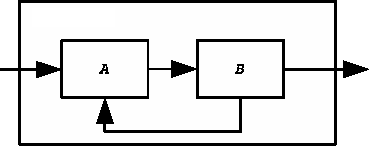
\includegraphics[trim=0cm 0cm 0cm 0cm, scale=0.7]{fig/coupled}
\caption{Spojovaný model tvořený atomickými modely A a B.}
\label{fig:coupled}
\end{figure}

\subsubsection{Formální definice}

\begin{math}
N=<X,Y,D,\{M_i\},C_{xx}, C_{yx}, C_{yy}, Select>
\end{math}

\begin{itemize}
\item $X$ - množina vstupních událostí.
\item $Y$ - množina výstupních událostí.
\item $D$ - množina jmen podkomponent této DEVS komponenty.
\item $M_i$ - množina podkomponent kde pro každou platí $i \in D$.
\item $C_{xx}\subseteq X \times \bigcup_{i \in D} X_i$ - množina externích vstupních propojení.
\item $C_{yx}\subseteq \bigcup_{i \in D} Y_i \times \bigcup_{i \in D} X_i$ - množina interních propojení.
\item $C_{yy}: \bigcup_{i \in D} Y_i \rightarrow Y^\phi$ - množina externích výstupních propojení.
\item $Select:2^D \rightarrow D$ - funkce určující, jak vybrat komponentu zpracovávající událost z množiny událostí naplánovaných na stejný čas.
\end{itemize}

Podobně jako atomické modely, mění i spojované modely stavy svých komponent v případě příchozí události nebo pokud jedna z podkomponent spustí svoji interní přechodovou funkci $\delta_{int}$ a vygeneruje výstup. V obou případech jsou tyto události přeposlány ostatním komponentám definovaným v množinách propojení $C_{xx}$, $C_{yy}$ a $C_{yx}$.

\subsubsection{Příklad využití formalismu DEVS}

Příklad simulace fronty v obchodním domě lze popsat pomocí formalismu DEVS. Jak lze vidět na obrázku \ref{fig:fronta}, jedná se o tři atomické modely propojené v rámci jednoho spojovaného modelu.

\begin{figure}[ht]
\centering
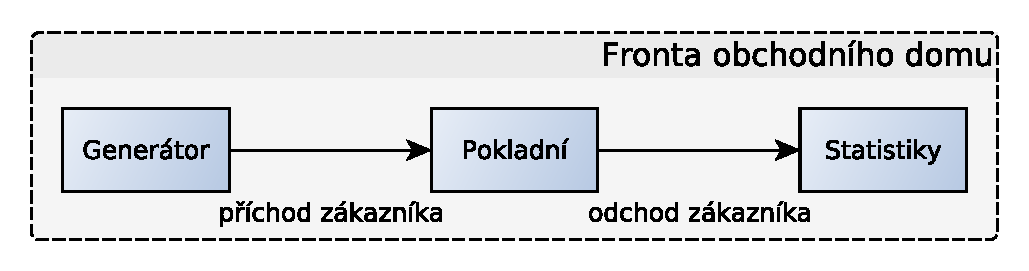
\includegraphics[trim=0cm 0cm 0cm 0cm, scale=0.7]{fig/fronta}
\caption{Model fronty obchodního domu popsaný pomocí formalismu DEVS.}
\label{fig:fronta}
\end{figure}

Atomický model Generátor zajišťuje generování zákazníků, kteří jsou pak přidáni na konec fronty. Zákazníci jsou v čase generováni pomocí náhodného rozložení. Model Generátor má jedinou výstupní událost nazvanou "příchod zákazníka", která je napojena na vstupní událost dalšího atomického modelu nazvaného Pokladní.

Atomický model Pokladní reprezentuje pokladního a jeho frontu. Při každé vstupní události "příchod zákazníka" je zavolána funkce externího přechodu a nový zákazník je uložen do fronty uvnitř tohoto modelu. Funkce posunu času plánuje následující událost modelu v závislosti na době zbývající k obsloužení aktuálního zákazníka.

Jakmile je zákazník obsloužen (tzv. po uplynutí doby definované funkcí posunu času), je nejprve zavolána výstupní funkce modelu. V této funkci je zákazník předán na výstup nazvaný "odchod zákazníka". Ihned po výstupní funkci je zavolána interní přechodová funkce. Tato funkce odebere obslouženého zákazníka z fronty a začne obsluhu následujícího zákazníka.

V případě, kdy zákazník příjde do fronty ve stejnou dobu jako je jiný zákazník obsloužen, je zavolána kolizní funkce. Tato kolize je řešena dokončením obsloužení aktuálního zákazníka a až pak přidáním nového zákazníka na konec fronty.

Posledním atomickým modelem je model Statistiky. Tento model obsahuje vstupní událost "odchod zákazníka", na kterou je napojena stejnojmenná výstupní událost modelu Pokladní. Úkolem tohoto modelu je uložit ve své externí přechodové funkci dobu, kterou každý zákazník strávil ve frontě a na konci simulace vypsat statistické informace.

\section{Knihovna ADEVS umožňující událostně řízenou simulaci}

V této podkapitole je stručně popsána knihovna ADEVS umožňující událostně řízenou simulaci. Vzhledem k povaze diplomové práce bylo potřeba využít open-source knihovnu podporující jazyk C++. Knihovna ADEVS je jako jediná aktivně vyvíjená knihovna schopna tyto požadavky splnit.

Jejím autorem je James J. Nutaro působící v Oak Ridge National Laboratory. Knihovna je vydána pod licencí LGPLv2+. Následující podkapitoly vychází z \cite{adevs}.

\subsection{Atomický model}

Atomický model formalismu DEVS je v knihovně ADEVS reprezentován třídu Atomic. Každý model (a tedy i třída Atomic) má své vstupy a výstupy. Jednotlivé vstupy a výstupy jsou definovány třídou PortValue. Tato třída popisuje pár klíč-hodnota, kde klíčem je celé číslo určující index vstupu nebo výstupu a hodnotou je typ dat na vstupu nebo výstupu.

V modelovém příkladu obchodního domu je hodnotou na vstupech a výstupech zákazník. Zákazníka, společně s podtřídou definující typ vstupů a výstupů, lze definovat následovně:

\lstset{language=XML, numbers=left, frame=single, breaklines=true, tabsize=2, xleftmargin=20pt, literate=%
    {á}{{\'a}}1
    {č}{{\v{c}}}1
    {ď}{{\v{d}}}1
    {é}{{\'e}}1
    {ě}{{\v{e}}}1
    {í}{{\'i}}1
    {ň}{{\v{n}}}1
    {ó}{{\'o}}1
    {ř}{{\v{r}}}1
    {š}{{\v{s}}}1
    {ť}{{\v{t}}}1
    {ú}{{\'u}}1
    {ů}{{\r{u}}}1
    {ý}{{\'y}}1
    {ž}{{\v{z}}}1
    {Á}{{\'A}}1
    {Č}{{\v{C}}}1
    {Ď}{{\v{D}}}1
    {É}{{\'E}}1
    {Ě}{{\v{E}}}1
    {Í}{{\'I}}1
    {Ň}{{\v{N}}}1
    {Ó}{{\'O}}1
    {Ř}{{\v{R}}}1
    {Š}{{\v{S}}}1
    {Ť}{{\v{T}}}1
    {Ú}{{\'U}}1
    {Ů}{{\r{U}}}1
    {Ý}{{\'Y}}1
    {Ž}{{\v{Z}}}1}
\begin{lstlisting}
struct Customer {
    double twait; // Čas potřebný pro obsloužení zákazníka
    double tenter, tleave; // Čas příchodu a odchodu zákazníka
};
// Definice typu vstupu a výstupů jednotlivých modelů
typedef adevs::PortValue<Customer*> IO_Type;
\end{lstlisting}

Třída Atomic definující atomický model vychází přímo z formalismu DEVS. Nový model vznikne vytvořením třídy dědící třídu Atomic, která implementuje jednotlivé funkce atomického modelu formalismu DEVS. Třída Atomic má tak následující metody, které je potřeba pro každý model definovat:

\begin{itemize}
\item delta\_int() - Metoda odpovídající funkci $\delta_{int}$ formalismu DEVS.
\item delta\_ext(...) - Metoda odpovídající funkci $\delta_{ext}$ formalismu DEVS.
\item delta\_conf(...) - Metoda odpovídající funkci $\delta_{conf}$ formalismu DEVS.
\item output\_func(...) - Metoda odpovídající funkci $\lambda$ formalismu DEVS.
\item ta() - Metoda odpovídající funkci $ta(s)$ formalismu DEVS.
\item gc\_output(...) - Metoda sloužící k odstranění nepotřebných objektů vytvořených v rámci ostatních metod.
\end{itemize}

Pro modelový příklad obchodního domu by pak kostra atomického modelu definujícího Pokladního vypadala následovně:

\lstset{language=XML, numbers=left, frame=single, breaklines=true, tabsize=2, xleftmargin=20pt, literate=%
    {á}{{\'a}}1
    {č}{{\v{c}}}1
    {ď}{{\v{d}}}1
    {é}{{\'e}}1
    {ě}{{\v{e}}}1
    {í}{{\'i}}1
    {ň}{{\v{n}}}1
    {ó}{{\'o}}1
    {ř}{{\v{r}}}1
    {š}{{\v{s}}}1
    {ť}{{\v{t}}}1
    {ú}{{\'u}}1
    {ů}{{\r{u}}}1
    {ý}{{\'y}}1
    {ž}{{\v{z}}}1
    {Á}{{\'A}}1
    {Č}{{\v{C}}}1
    {Ď}{{\v{D}}}1
    {É}{{\'E}}1
    {Ě}{{\v{E}}}1
    {Í}{{\'I}}1
    {Ň}{{\v{N}}}1
    {Ó}{{\'O}}1
    {Ř}{{\v{R}}}1
    {Š}{{\v{S}}}1
    {Ť}{{\v{T}}}1
    {Ú}{{\'U}}1
    {Ů}{{\r{U}}}1
    {Ý}{{\'Y}}1
    {Ž}{{\v{Z}}}1}
\begin{lstlisting}
class Clerk: public adevs::Atomic<IO_Type>  {
    public:
        Clerk();
        ~Clerk();

        void delta_int();
        void delta_ext(double e, adevs::Bag<IO_Type>& xb);
        void delta_conf(adevs::Bag<IO_Type>& xb);
        void output_func(adevs::Bag<IO_Type>& yb);
        double ta();
        void gc_output(adevs::Bag<IO_Type>& g);
        
        static const int arrive; // Index vstupního portu
        static const int depart; // Index výstupního portu
    private:
        double t; // Simulační čas
        list<Customer*> line; // Seznam zákazníků ve frontě
        double t_spent; // Čas strávený s aktuálním zákazníkem
};
\end{lstlisting}

Typ adevs::Bag je abstraktním datovým typem umožňujícím uchování jakýchkoliv objektů (v tomto případě objektů typu IO\_Type). Implementace jednotlivých metod by vycházela z popisu chování modelu Pokladního.

Kostra dalších modelů (Generator a Statistics) v simulaci obchodního domu se příliš neliší od modelu zákazníka.

\subsection{Spojovaný model}

Spojovaný model je v knihovně ADEVS reprezentován třídou Network. Standardně nabízí knihovna ADEVS implementaci této třídy nazvanou SimpleDigraph. Pomocí této třídy lze propojovat vstupní a výstupní porty jednotlivých atomických i spojovaných modelů. Využití této třídy je přímočaré, jak ilustruje následující ukázka propojující modely Generator a Clerk:

\lstset{language=XML, numbers=left, frame=single, breaklines=true, tabsize=2, xleftmargin=20pt, literate=%
    {á}{{\'a}}1
    {č}{{\v{c}}}1
    {ď}{{\v{d}}}1
    {é}{{\'e}}1
    {ě}{{\v{e}}}1
    {í}{{\'i}}1
    {ň}{{\v{n}}}1
    {ó}{{\'o}}1
    {ř}{{\v{r}}}1
    {š}{{\v{s}}}1
    {ť}{{\v{t}}}1
    {ú}{{\'u}}1
    {ů}{{\r{u}}}1
    {ý}{{\'y}}1
    {ž}{{\v{z}}}1
    {Á}{{\'A}}1
    {Č}{{\v{C}}}1
    {Ď}{{\v{D}}}1
    {É}{{\'E}}1
    {Ě}{{\v{E}}}1
    {Í}{{\'I}}1
    {Ň}{{\v{N}}}1
    {Ó}{{\'O}}1
    {Ř}{{\v{R}}}1
    {Š}{{\v{S}}}1
    {Ť}{{\v{T}}}1
    {Ú}{{\'U}}1
    {Ů}{{\r{U}}}1
    {Ý}{{\'Y}}1
    {Ž}{{\v{Z}}}1}
\begin{lstlisting}
adevs::Digraph<Customer*> store;
Clerk* clrk = new Clerk();
Generator* genr = new Generator();
// Přidání atomických modelů do spojovaného modelu "store"
store.add(clrk); 
store.add(genr);
// Propojení výstupu generátoru se vstupem pokladního
store.couple(genr, genr->arrive, clrk, clrk->arrive);
\end{lstlisting}

Zbylé modely by byly propojeny analogicky. Tímto způsobem lze pomocí mnoha dílčích atomických modelů vytvářet rozsáhlé komunikující systémy.

Simulaci lze pak pomocí další třídy Simulator knihovny ADEVS spustit a krokovat:

\lstset{language=XML, numbers=left, frame=single, breaklines=true, tabsize=2, xleftmargin=20pt, literate=%
    {á}{{\'a}}1
    {č}{{\v{c}}}1
    {ď}{{\v{d}}}1
    {é}{{\'e}}1
    {ě}{{\v{e}}}1
    {í}{{\'i}}1
    {ň}{{\v{n}}}1
    {ó}{{\'o}}1
    {ř}{{\v{r}}}1
    {š}{{\v{s}}}1
    {ť}{{\v{t}}}1
    {ú}{{\'u}}1
    {ů}{{\r{u}}}1
    {ý}{{\'y}}1
    {ž}{{\v{z}}}1
    {Á}{{\'A}}1
    {Č}{{\v{C}}}1
    {Ď}{{\v{D}}}1
    {É}{{\'E}}1
    {Ě}{{\v{E}}}1
    {Í}{{\'I}}1
    {Ň}{{\v{N}}}1
    {Ó}{{\'O}}1
    {Ř}{{\v{R}}}1
    {Š}{{\v{S}}}1
    {Ť}{{\v{T}}}1
    {Ú}{{\'U}}1
    {Ů}{{\r{U}}}1
    {Ý}{{\'Y}}1
    {Ž}{{\v{Z}}}1}
\begin{lstlisting}
adevs::Simulator<IO_Type> sim(&store);
while (sim.nextEventTime() < DBL_MAX) {
    sim.execNextEvent();
}
\end{lstlisting}

Takto lze za pomocí knihovny ADEVS vytvořit jednoduchý modulární simulátor a řídit simulaci.

\chapter{Návrh událostně řízeného simulátoru}
\label{navrh}

Cílem této kapitoly je popsat strukturu navrženého simulátoru, jeho rozhraní pro komunikaci s periferiemi a mikrokontrolerem a knihovnu implementující mikrokontroler MSP430. Je zde také zmíněno grafické uživatelské rozhraní simulátoru.

\section{Struktura navrženého simulátoru}

Simulátor bude rozdělen do čtyř navzájem se doplňujících částí - simulační jádro, knihovna simulující MCU MSP430, komponenty rozšiřující simulační jádro a grafické uživatelské rozhraní. Toto rozdělení lze vidět na obrázku \ref{fig:struktura}.

\begin{figure}[ht]
\centering
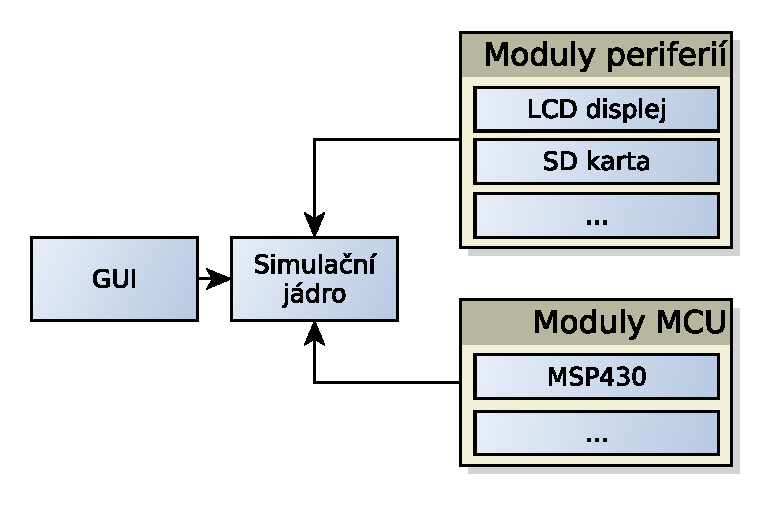
\includegraphics[trim=0cm 0cm 0cm 0cm, scale=0.7]{fig/struktura}
\caption{Struktura navrženého simulátoru.}
\label{fig:struktura}
\end{figure}

Simulační jádro bude založeno na formalismu Spojovaného DEVS a bude umožňovat propojení všech simulovaných komponent. Komponenty budou atomickými modely formalismu DEVS a budou implementovat chování jednotlivých simulovaných periferií jako například tlačítka, LCD displeje nebo i samotného mikrokontroleru. Mikrokontroler bude vzhledem ke své komplexnosti implementován jako nezávislá knihovna. Grafické uživatelské rozhraní pak zpřístupní všechny funkce simulátoru uživateli.

\section{Návrh simulačního jádra}

Simulační jádro bude sloužit k řízení simulace, přeposílání zpráv mezi komponentami a umožní propojení simulovaných komponent (jednoho mikrokontroleru a více periferií). Každá komponenta bude samostatným modulem a bude mít pevně dané rozhraní pro komunikaci s jinými komponentami vyplývající z atomického modelu formalismu DEVS.

Vstupní a výstupní události definované ve formalismu DEVS budou chápány jako změny napětí na konkrétních pinech komponent. Propojení realizovaná pomocí Spojovaného DEVS pak budou reprezentovat propojení pinů komponent.

Každá komponenta bude schopna následujícího chování:

\begin{itemize}
\item Změnit svůj vnitřní stav na základě změny simulačního času - $ta$ funkce z definice formalismu DEVS.
\item Změnit svůj vnitřní stav na základě externí události přijaté na vstupní port (typicky na základě zprávy od jiné komponenty) - $\delta_{int}$ funkce z formalismu DEVS.
\item Generovat zprávy na výstupní port - $\lambda$ funkce z formalismu DEVS.
\end{itemize}

Mikrokontroler bude speciálním rozšířením běžné komponenty poskytujícím navíc přístup ke své paměti, regitrům a kódu programu. To umožní řídit simulaci na základě instrukcí a obsahu paměti a registrů daného mikrokontroleru. V rámci celé simulace bude existovat jen jedna instance mikrokontroleru.

Simulační jádro bude umět komponenty dynamicky načítat aniž by docházelo k jeho jakékoliv úpravě. Návrh je tak velmi obecný a umožní snadné přidávání dalších rozšiřujících komponent nebo i simulaci jiného mikrokontroleru.

% \subsection{Komponenty}
% 
% Komponenta je nejmenší simulovatelná část systému. Komponenty jsou navrženy jako samostatné moduly s pevně daným rozhraním, pomocí kterého komunikují s ostatními komponentami simulace. Návrh je tak velmi obecný a umožňuje přidávání dalších rozšiřujících komponent.
% Návrh počítá se dvěma typy komponent:
% 
% \begin{itemize}
% \item \textbf{Periferie} - Je jakákoliv simulační komponenta, která umí reagovat na zprávy přijímané od jiných periférií, generovat nové zprávy a měnit svůj vnitřní stav na základě simulačního času.
% \item \textbf{Mikrokontroler (MCU)} - Jedná se o speciální případ periferie, která obsahuje paměť, registry a kód programu, který vykonává.
% To umožní řídit simulaci na základě instrukcí, obsahu paměti a registrů daného mikrokontroléru.  V rámci celé simulace je jen jedna instance mikrokontroleru. 
% \end{itemize}
% 
% Každá komponenta (periferie) tak bude schopna následujícího chování:
% 
% \begin{itemize}
% \item Změnit svůj vnitřní stav na základě změny simulačního času.
% \item Změnit svůj vnitřní stav na základě externí události přijaté na vstupní port (typicky na základě zprávy od jiné komponenty).
% \item Generovat zprávy na výstupní port.
% \end{itemize}
% 
% Mikrokontrolery navíc oproti periferiím budou poskytovat následující informace:
% 
% \begin{itemize}
% \item Obsah paměti a registrů.
% \item Disassemblovaný kód běžícího programu.
% \end{itemize}
% 
% Vstupní a výstupní porty definované ve formalismu DEVS budou představovat jednotlivé piny komponent. Spojení mezi porty pak bude značit spojení jednolivých
% pinů a zprávy posílané mezi porty budou reprezentovat aktuální napětí na pinech.

% Na obrázku .... lze vidět ukázku propojení dvou komponent (mikrokontroleru MSP430 a periferie - LED diody). Pokud program mikrokontroleru vygeneruje na svůj 
% výstupní port hodnotu 3.3 (tzv. 3.3 voltu), bude tato zprávy předána na vstupní port LED diody, která na jejím základě změní svůj vnitřní stav (tzv. rozsvítí se).

\section{Návrh knihovny simulující MCU MSP430}

Knihovna simulující mikrokontroler MSP430 je klíčovou částí projektu. Bude umožňovat nahrání uživatelského programu a jeho
následnou simulaci pomocí vykonávání instrukcí a běhu svých dalších interních komponent. Tato simulace bude řízena simulačním jádrem. Knihovna také poskytne grafickému uživatelskému rozhraní přístup ke své paměti a registrům, čímž umožní krokování programů. Bude také nabízet přístup k dalším ladícím informacím jako je například umístění lokálních a globálních proměnných v paměti nebo v registrech s využitím DWARF ladících informací.

Na obrázku \ref{fig:msp430_arch} lze vidět základní schéma MSP430 knihovny a její dekompozici. V této podkapitole jsou jednotlivé části tohoto schématu podrobněji rozebrány s důrazem na jejich funkci a postavení v rámci celé MSP430 knihovny.

\begin{figure}[ht]
\centering
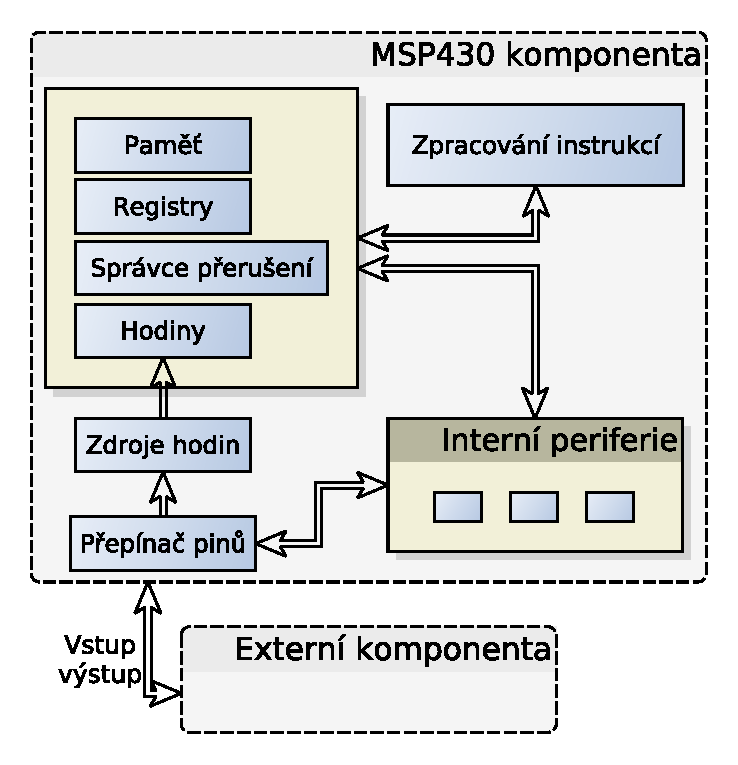
\includegraphics[trim=0cm 0cm 0cm 0cm, scale=0.7]{fig/msp430_arch}
\caption{Návrh architektury MSP430 komponenty.}
\label{fig:msp430_arch}
\end{figure}

\subsection{Paměť}

Paměť slouží k uchování jak uživatelského programu tak dat. Ostatní části mikrokontroleru (zejména pak interní periferie jako například USI nebo USCI) musí být schopny do paměti zapisovat jak slova tak jednotlivé byty a být informovány o případném čtení nebo zápisu provedeném uživatelským programem. To je podstatná vlastnost například pro automatické smazání příznaku přerušení po jeho přečtení. Dalším možným využitím informování o zápisu do paměti je možnost zastavení simulace po změně hodnoty v paměti a tím lepší možnost ladit uživatelský program.

Do paměti musí být umožněno načtení uživatelského programu ve formátu A43. Načítání programu z ELF souboru bude probíhat jeho převodem na formát A43 a následným načtením.

\subsection{Registry}

Návrh registrů, podobně jako návrh paměti, počítá s možností čtení a zápisu jednoho nebo dvou bytů. Opět je potřeba umožnit ostatním částem mikrokontroleru zjistit, že došlo k zápisu do registru. Typickým předpokládaným využitím je krokování programu na základě hodnoty PC registru. Další možné využití může být monitorování stavového registru a zastavení simulace při určitém příznaku.

\subsection{Přepínač pinů}

Každá varianta mikrokontroleru obsahuje různé interní periferie a tím pádem i jiný počet pinů a jejich rozmístění na pouzdru mikrokontroleru. Na jeden pin může být zapojeno více interních periferií a to, která periferie právě daný pin obsluhuje, je určeno za pomocí řídících registrů (například PxSEL a PxSEL2).

Jednotlivé varianty mikrokontroleru MSP430 budou z hlediska pinů a jejich připojení na interní periferie popsány v XML souboru, který bude obsahovat o každém pinu následující informace:

\begin{itemize}
\item Umístění pinu na pouzdru mikrokontroleru (vlevo, vpravo, ...) včetně jeho pořadí na dané straně pouzdra.
\item Seznam názvů vstupů/výstupů realizovaných pomocí pinu a hodnoty bitů v řídících registrech určujících, který vstup/výstup bude kdy zvolen.
\end{itemize}

Interní komponenty (například časovač nebo modul USI) budou mít zaregistrovány v přepínači pinů názvy svých vstupů a výstupů.
Přepínač pinů pak bude na základě aktuálně simulované varianty MSP430 mikrokontroleru monitorovat řídící registry PxSEL, PxSEL2, atd. a podle jejich hodnoty přeposílat vstupy z externích komponent konkrétním interním periferiím (princip multiplexoru). Tento princip ilustruje obrázek \ref{fig:msp430_pinmult}.

\begin{figure}[h]
\centering
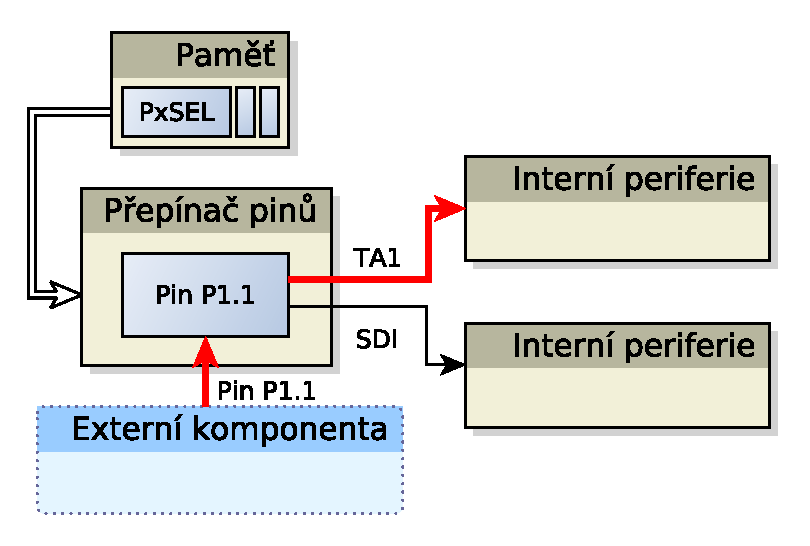
\includegraphics[trim=0cm 0cm 0cm 0cm, scale=0.7]{fig/msp430_pinmult}
\caption{Přepínač pinů přeposílá vstup z externí komponenty na interní periferii podle hodnoty PxSEL.}
\label{fig:msp430_pinmult}
\end{figure}

Přepínač pinů bude rovněž směrovat signály uvnitř MSP430 komponenty. Toho bude potřeba pro interní propojení jednotlivých interních periferií (například výstup časovače může být použit jako vstup modulu USI - toto propojení se děje uvnitř MSP430 komponenty bez využití externích pinů).

\subsection{Zdroje hodin}

Zdroje hodin budou generovat hodinový signál o určité frekvenci. Tento signál pak bude sloužit hodinám (MCLK, SMCLK a ACLK) pro řízení jednotlivých částí mikrokontroleru. Z hlediska simulace je možné zdroje hodin rozdělit na dvě kategorie. Zdroje závislé na externích komponentách (LFXT1CLK, XT2CLK) a zdroje závislé pouze na čase (VLOCLK, DCOCLK).

Zdroje závislé na externích komponentách musí být schopny přijímat zprávy od externích komponent a na jejich základě pak generovat hodinový signál, který je dále zpracován jednotlivými hodinami.

Zdroje závislé na čase musí být samostatnými simulačními komponentami a musí samy na základě uběhnutého času generovat hodinový signál s patřičnou frekvencí.

Všechny zdroje hodin musí generovat informace jak o náběžné, tak o sestupné hraně hodinového signálu. To je podstatná vlastnost například pro modul USI, který provádí své akce s oběma hranami hodinového signálu.

\subsection{Hodiny}

Hodiny (MCLK, SMCLK a ACLK) dále zpracovávají hodinový signál od zdrojů hodinového signálu. Umožňují nastavit děličku, čímž mění frekvenci hodinového signálu. K jednotlivým hodinám budou připojeny interní periferie, které jimi budou řízeny. Stejně jako u zdrojů hodinového signálu je potřeba u zdrojů hodin poskytovat informace jak o náběžné tak o sestupné hraně.

\subsection{Správce přerušení}

Správce přerušení bude udržovat informace o požadavcích na přerušení. Modulu zpracovávajícímu instrukce umožní spustit rutinu přerušení, pokud je nějaké
přerušení ve frontě. Ostatním interním komponentám pak umožní žádat o přerušení.

Interní komponenty budou rovněž potřebovat informaci o dokončení konkrétního typu přerušení (například pro vymazání příznaku přerušení po jeho obsluze).

\subsection{Zpracování instrukcí}

Zpracování instrukcí ilustruje diagram na obrázku \ref{fig:msp430_inst}.

\begin{figure}[h]
\centering
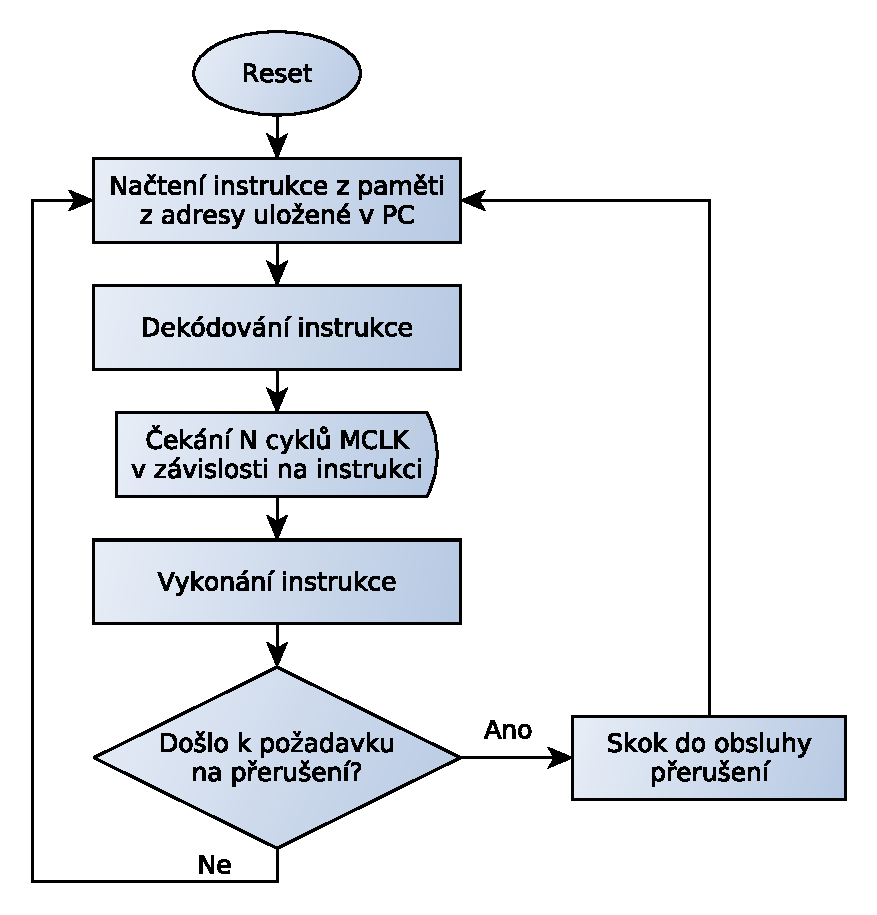
\includegraphics[trim=0cm 0cm 0cm 0cm, scale=0.7]{fig/msp430_inst}
\caption{Diagram zpracování instrukcí.}
\label{fig:msp430_inst}
\end{figure}

Z obrázku lze vidět, že je zpracování instrukce rozděleno na několik částí. Nejprve je instrukce načtena z paměti v závislosti na hodnotě registru PC (R0).
Dále dojde k dekódování instrukce a jejímu vykonání. Vykonání instrukce je atomické a trvá několik MCLK cyklů. Počet cyklů potřebných pro vykonání
instrukce je znám již po jejím dekódování. Proto je mezi dekódováním a vykonáním vloženo čekání simulující vykonávání instrukce na reálném HW.
Po vykonání instrukce je potřeba obsloužit jakákoliv přerušení, která mohla v mezičase nastat. Tento cyklus se bude opakovat stále dokola, dokud MCLK generuje další pulsy (tzv. dokud simulace běží).

\subsection{Interní periferie}

Interní periferie budou využívat modulů popsaných dříve v této kapitole. Každá interní periferie tak bude mít přístup k paměti, registrům, pinům, správci
přerušení a hodinovému signálu. V rámci diplomové práce bude z interních periferií implementován časovač, modul a SPI komunikace za pomocí modulů USI, USCI a USART.

Jako příklad návrhu interní periferie se tato podkapitola věnuje pouze časovači. Princip návrhu ostatních periferií je však obdobný, liší se pouze jejich funkcí.

\subsubsection{Časovač}

Časovač bude monitorovat své řídící registry prostřednictvím paměťového modulu a v případě jejich změny, způsobené uživatelským programem, změní také své nastavení (výběr módu, vstupů atd.). Pro generování nastavení Capture overflow bitu (indikace situace, kdy uživatelský program nestihl přečíst hodnotu časovače během 2 přerušení) je potřeba vědět, zda uživatelský program přečetl aktuální hodnotu časovače. To bude řešeno opět pomocí paměťového modulu, kdy tento bude informovat časovač o přečtení dané hodnoty z paměti.

Časovač musí být schopen zvyšovat svoji hodnotu v závislosti na frekvenci. Proto bude časovač napojen na modul hodin (SMLK nebo ACLK). S každým cyklem
hodin pak v závislosti na svém nastavení vykoná danou funkci.

Pomocí časovače lze rovněž generovat pulsy na výstupních pinech umístěných na pouzdře mikrokontroleru a vzorkovat napětí na pinech vstupních.
Je proto nutné umožnit časovači přístup k těmto pinům. To bude provedeno pomocí přepínače pinů. Časovač si zaregistruje potřebné názvy vstupů a výstupů
a přepínač pinů pak v závislosti na akcích uživatelského programu bude směrovat vstupy mikrokontroleru přímo do časovače.

Přerušení časovače budou generována pomocí správce přerušení. Je však potřeba zajistit, aby se časovač dozvěděl o dokončení rutiny obsluhující přerušení
(přerušení časovače je sdíleno více zdroji přerušení a časovač musí být schopen požádat o další přerušení z jiného zdroje ihned po obsloužení původního přerušení). Toto je zajištěno monitorováním ukončených přerušení pomocí správce přerušení.

Z příkladu časovače lze vidět, že návrh a dekompozice mikrokontroleru MSP430 je dostačující pro interní periferie a poskytuje všechny potřebné vlastnosti.

\section{Návrh grafického uživatelského rozhraní}

Hlavní funkcí grafického uživatelského rozhraní bude řízení simulace, jednoduchá editace jednotlivých simulovaných komponent a ladění programu mikrokontroleru.

Grafické uživatelské rozhraní by tedy mělo mít následující funkce:

\begin{itemize}
\item \textbf{Správa projektu} - Vytvoření, uložení a nahrání projektu.
\item \textbf{Editace projektu} - Přidávání a odebírání simulovaných komponent a editace jejich propojení.
\item \textbf{Řízení simulace} - Nastavení parametrů simulace, kontrola jejího běhu, krokování atd.
\item \textbf{Ladění programu} - Zobrazení zdrojového kódu programu, hodnoty proměnných, registrů, paměti.
\item \textbf{Ladění signálů} - Možnost kontrolovat v čase signály přenášené mezi simulovanými komponentami.
\end{itemize}

V této kapitole jsou tyto požadavky kladené na grafické uživatelské rozhraní detailně rozebrány a je navrženo grafické uživatelské rozhraní, které tyto
požadavky splňuje.

\subsection{Základní koncepce}

Nejdůležitější součástí hlavního okna simulátoru bude kreslící plocha. Na této ploše budou vykresleny jednotlivé simulované komponenty (mikrokontroler
a periferie) včetně jejich pinů a propojení mezi piny. Uživatel bude schopen přidávat nové komponenty a odstraňovat stávající, propojovat je pomocí
vodičů a měnit jejich vlastnosti (například barvu LED diody). Během simulace se budou všechny komponenty aktualizovat a uživatel tak uvidí průběh simulace
(LED dioda bude blikat, aktivní piny budou zobrazeny rozdílnou barvou než piny neaktivní atd.).

Další důležitou částí grafického uživatelského rozhraní bude zobrazení zdrojového kódu programu nahraného v mikrokontroleru. Tento kód bude poskytnut
přímo mikrokontrolerem a GUI jej pouze zobrazí. Z principu lze vždy zobrazit kód v assembleru. Pokud však bude dostupný zdrojový kód v jazyce C, bude 
simulátor schopen přepínat mezi kódem v assembleru a kódem v C. Po zastavení simulace se zobrazí aktuální instrukce (případně odpovídající příkaz v jazyce C). Uživatelské rozhraní bude rovněž umožňovat nastavení breakpointů (bodů zastavení) na jednotlivých instrukcích, čímž umožní jednodušší krokování
simulace.

Pro zobrazení interních informací o jednotlivých simulovaných komponentách bude sloužit třetí část uživatelského rozhraní. Půjde o strukturovaný seznam
typu název-hodnota, který bude zobrazovat informace o aktuálních hodnotách registrech mikroprocesoru, důležitých místech v paměti, nebo například hodnotách
lokálních proměnných v místě zastavení simulace. Každá komponenta bude schopna přidat do tohoto seznamu své položky a předávat tak uživateli potřebné
interní informace.

Poslední dílčí částí uživatelského rozhraní bude rozhraní pro zobrazení napětí na jednotlivých pinech formou osciloskopu. Uživatel si bude moci vybrat
piny, které chce během simulace sledovat a během simulace (nebo i po jejím zastavení) uvidí veškeré změny signálu, které se na pinech odehrály.

\subsection{Správa projektu}

Při vytvoření nového projektu bude uživatel dotázán na vybrání jeho architektury (návrh celé aplikace se neomezuje pouze na mikrokontrolery rodiny MSP430) a varianty dané architektury (v případě mikrokontroleru MSP430 se bude jednat o jeho konkrétní typ). Po vytvoření projektu uvidí uživatel na kreslící ploše vybraný mikrokontroler a bude mu umožněno nahrání programu a přidání dalších periferií.

Při uložení projektu bude potřeba uložit informace o všech komponentách, jejich propojení a umístení na kreslící ploše. Budou se rovněž ukládat informace
o aktuálně používaných breakpointech a sledovaných pinech.

\subsection{Editace projektu}

Editace projektu bude probíhat na kreslící ploše zobrazující všechny komponenty. Na kreslící plochu bude možné přidávat nové periferie ze seznamu periferií, případně ostraňovat periferie stávající. Uživateli bude umožněno periferiemi volně pohybovat po kreslící ploše a propojovat jejich piny pomocí vodičů. Bude možné propojit i více než 2 piny (lze tak vytvořit sběrnicovou topologii s uzly). Propojení mezi piny bude možné odstraňovat.

\subsection{Řízení simulace}

Grafické uživatelské rozhraní umožní spuštění simulace, její dočasné zastavení a její restartování. Během simulace bude uživateli prezentován aktuální simulační čas a uvidí změny simulovaného zapojení na kreslící ploše a osciloskopu. Při dočasném zastavení simulace uvidí uživatel aktuální
stav simulovaného zapojení (stav všech registrů a paměti, následující instrukci ve zdrojovém kódu atd.). Simulaci bude také možné automaticky zastavit po určitém simulačním čase.

K dispozici bude také funkce pro krokování programu s následujícími 3 módy:

\begin{itemize}
\item \textbf{Událost simulace} - Provede další událost v simulaci. Jedná se například o jeden tik hodin MCLK, nebo 1 tik externího oscilátoru. Jedna událost je nejmenší možný krok, jaký lze v diskrétní simulaci provést.
\item \textbf{Instrukce} - Provede další instrukci mikrokontroleru. Instrukce zpravidla trvá více simulačních kroků, půjde tedy o méně jemné krokování simulace.
\item \textbf{Řádek v jazyce C} - Provádí instrukce mikrokontroleru, dokud tyto implementují stále tentýž řádek ve zdrojovém souboru v jazyce C. Při volbě tohoto krokování musí být výsledná aplikace schopna detekovat cykly (například 1 instrukce NOP opakující se stále dokola ve smyčce), aby nedošlo k zamrznutí simulace při vykonávání kroku.
\end{itemize}

Další možností pozastavení simulace jsou takzvané breakpointy. Uživatel musí umět nastavit pozastavení simulace v případě, kdy určitý registr nabyl jím definovanou hodnotu (případně když hodnota v paměti definovaná adresou nabyla konkrétní hodnotu).

\subsection{Ladění programu}

Při každém pozastavení simulace uvidí uživatel aktuální instrukci ve zdrojovém kódu. Kromě samotného zdrojového kódu mu budou zobrazeny, pokud byl nahrán program ve formátu ELF s ladícími symboly, názvy všech zdrojových souborů nahraného programu a všech funkcí v daných souborech. Uživatel bude moci vybrat daný soubor a funkci v něm pro rychlejší orientaci v projektu. V případě dostupnosti zdrojového kódu v jazyce C se uživateli zobrazí jeho kód. Vždy však bude možné zobrazit diassemblovaný kód v assembleru. Uživatel bude moci přidávat breakpointy v libovolných místech kódu a po opětovném spuštění simulace se tato zastaví na místě, které uživatel zvolil.

V grafickém uživatelském rozhraní budou rovněž zobrazeny hodnoty registrů a důležitých adres v paměti (standardně hexadecimálně, avšak bude možné zobrazit jejich hodnoty i v jiných soustavách). Uživatel bude moci použít tento seznam registrů a míst v paměti pro rychlé přidání nových breakpointů. Na základě místa ve zdrojovém kódu, na kterém došlo k pozastavení simulace, budou zobrazeny jména a hodnoty lokálních proměnných.

\subsection{Ladění signálů}

Uživateli bude umožněno vybrání pinů na kreslící ploše a jejich zařazení do seznamu sledovaných pinů. V pruběhu simulace se změny napětí na sledovaných pinech budou ukládat a zobrazovat uživateli v graficky pomocí rozhraní podobného osciloskopu. Uživatel tak uvidí vztahy mezi jednotlivými signály generovanými na pinech v závislosti na čase. Standardně bude rozhraní ukazovat průběh celé simulace. Bude však možné určitý časový úsek přiblížit a získat tak detailnější pohled.

\chapter{Implementace událostně řízeného simulátoru}

Cílem této kapitoly je popsat výsledný implementovaný simulátor založený na předešlém návrhu. Jako výchozí jazyk byl zvolen jazyk C++. Jedná se o jazyk podporující objektově orientované programování (OOP), čímž zjednodušuje dekompozici celého projektu na menší celky. Nástroj QDevKit, který může v budoucnu implementovaný simulátor rozšířit, je rovněž programován v jazyce C++, takže bude jejich budoucí spravování jednodušší.

Pro tvorbu grafického uživatelského rozhraní byla použita knihovna Qt \cite{qt}. Jedná se o multiplatformní knihovnu použitou i v projektu QDevKit licencovanou pod licencí LGPL.

V následujících kapitolách jsou popsány implementační detaily jednotlivých částí simulátoru. Vzhledem k rozsáhlosti celého projektu se tato kapitola soustředí pouze na nejzajímavější aspekty implementace a nepopisuje implementaci do úplných detailů.

\section{Simulační jádro}

Jako základ pro simulační jádro byla použita knihovna ADEVS. Tato knihovna implementuje diskrétní simulaci za pomocí formalismu DEVS a je šířena pod licencí GPLv2+. Díky této licenci může být použita i v případě bližší integrace simulátoru do prostředí QDevKit. Příklady využití knihovny ADEVS včetně její specifikace jsou k dispozici v rámci \cite{nutaro} a \cite{adevs}.

\subsection{Knihovna ADEVS a její využití}

Hlavní třídou knihovny ADEVS je třída adevs::Simulator. Tato třída určuje typ událostí, které se mezi jednotlivými simulovanými komponentami přeposílají a umožňuje řídit simulaci (lze například získat čas následující události a vykonat ji). Mezi komponentami se posílají události typu double (desetinné číslo),  které určují velikost napětí. Existuje zde však také speciální hodnota, která určuje stav vysoké impedance - DBL\_MAX.

Atomické modely formalismu DEVS jsou reprezentovány třídou adevs::Atomic. Tato třída obsahuje následující metody známé z formalismu DEVS:

\begin{itemize}
\item \textbf{delta\_int(...)} - metoda volána v případě změny interního stavu modelu.
\item \textbf{delta\_ext(...)} - metoda volána v případě externí události generované jiným modelem (jinou komponentou).
\item \textbf{output\_func(...)} - metoda volána v případě, kdy má model vygenerovat své výstupní události.
\item \textbf{ta(...)} - metoda určující čas setrvání v aktuálním stavu.
\end{itemize}

Každá simulovaná komponenta tak musí být dceřinou třídou třídy adevs::Atomic. Při spuštění (nebo restartování simulace) se musí veškeré komponenty a jejich propojení vytvořit znovu, protože mohly být v grafickém uživatelském rozhraní přidány nové komponenty a změněny jejich dosavadní propojení.

To představuje problém, protože, jak lze vidět na obrázku \ref{fig:adevs_classes}, komponenta není tvořena pouze simulační částí (tzv. třídou adevs::Atomic), ale i mnoha dalšími třídami, jejichž chování dědí (je například nutné komponenty vykreslovat v grafickém uživatelské rozhraní - dědit tomu odpovídající třídu). Není však optimální vytvářet objekty v grafickém uživatelském rozhraní znovu při každém restartování simulace.

Tento problém byl vyřešen oddělením simulační části komponenty do samostatné třídy SimulationObjectWrapper dědící ze třídy adevs::Atomic a využívající návrhový vzor Proxy. Tato třída mapuje volání metod třídy adevs::Atomic na volání třídy SimulationObject, ze které pak všechny simulované komponenty dědí
své chování. Tento vztah znázorňuje obrázek \ref{fig:adevs_classes}. Při restartování simulace tak nemusí být smazána a znovu vytvořena celá komponenta (třída SimulationObject), ale pouze třída SimulationObjectWrapper.

Třída adevs::Simulator potřebuje ke svému běhu také instanci třídy adevs::Network. Tato třída reprezentuje formalismus Spojovaného DEVS a definuje sadu čistě virtuálních metod \cite{oop}, které pak dceřiné třídy implementují (například pomocí metody route(...) se směrují události mezi komponentami). Knihovna ADEVS obsahuje několik implementací této třídy.

Bohužel jsou však tyto implementace velmi obecné a tím pádem i pomalé. Bylo tak nutné vytvořit novou třídu SimulationModel, která pracuje přímo s objekty typu SimulationObjectWrapper.

\subsection{Rozšiřitelné periferie formou modulů}

Jak již bylo zmíněno v předchozí podkapitole, každá simulovaná komponenta je dceřinou třídou třídy SimulationObject. Rozšiřitelné moduly umožňují načtení implementace této třídy ze sdílené knihovny nebo z kódu modulu v jazyce Python.

Protože je každou komponentu potřeba vykreslit v grafickém uživatelském rozhraní a umožnit interakci uživatele, musí rozšiřitelný modul implementovat rovněž třídu ScreenObject (tato je popsána dále v kapitole \ref{kreslici_plocha}). Pro jednoduchost byly tyto dvě třídy zapouzdřeny v třídě Peripheral, která je výslednou třídou pro implementaci rozšiřitelných modulů. Vztahy mezi popsanými třídami je možné vidět na obrázku \ref{fig:adevs_classes}

\begin{figure}[ht]
\centering
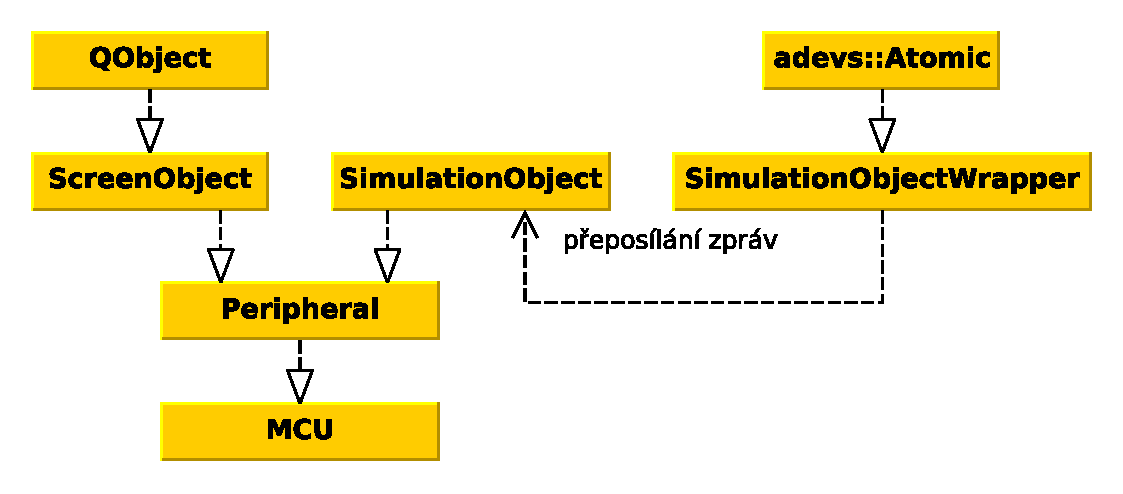
\includegraphics[trim=0cm 0cm 0cm 0cm, scale=0.7]{fig/adevs_class}
\caption{Diagram znázorňující vztahy mezi třídami knihovny ADEVS, simulovanými periferiemi a mikrokontrolery.}
\label{fig:adevs_classes}
\end{figure}

Každý modul obsahuje XML soubor obsahující jeho metadata. Jedná se zejména o jméno modulu, jméno autora, typ modulu (Pyhon nebo dynamická knihovna), název knihovny a licence. Tento XML soubor je načten třídou PeripheralManager a na základě metadat je pak dále nahrán jeho kód. Nahrání kódu modulu se liší v závislosti na typu modulu a je popsáno v následujících dvou podkapitolách.

Na základě metadat a nahraného kódu modulu je vytvořena instance třídy PeripheralInfo, kterou pak využívají další části simulátoru. Tato třída obsahuje metodu pro vytvoření nové instance periferie a poskytuje o periferii základní informace (například jméno). Seznam všech nahraných modulů lze pak získat pomocí již zmíněné třídy PeripheralManager.

\subsubsection{Moduly v jazyce C++}

Moduly naprogramované v jazyce C++ jsou načítány jako sdílené knihovny pomocí třídy QPluginLoader poskytované knihovnou Qt. Při programování C++ modulů je potřeba kromě třídy Peripheral implementovat rovněž třídu PeripheralInterface (s jedinou metodou create(...)), která slouží pro vytváření nových instancí periferií a kterou QPluginLoader používá k identifikaci modulu.

Ukázku kódu v jazyce C++ implementující jednoduché periferie lze najít v kapitole \ref{oscilator}.

\subsubsection{Moduly v jazyce Python}

Pro vytváření modulů v jazyce Python je využita knihovna PythonQt. Tato knihovna poskytuje rozhraní mezi Qt knihovnou a jazykem Python. Je rovněž použita v projektu QDevKit a tak při případné distribuci obou aplikací současně není přidávána žádná nová závislost.

Základ pro tvorbu modulů v jazyce Python byl převzat z projektu QDevKit (jedná se o třídy Script a ScriptEngine), avšak byly provedeny výkonostní optimalizace.

Pomocí třídy ScriptEngine jsou načteny moduly v jazyce Python třídou PeripheralManager a jsou dále reprezentovány jako instance třídy Script. Nad třídou Script jsou implementovány třídy PythonPeripheralInterface (rozšiřující třídu PeripheralInterface) a PythonPeripheral (rozšiřující třídu Peripheral).

Třída PythonPeripheralInterface vytváří novou instanci třídy PythonPeripheral, čímž vznikne nová periferie. Třída PythonPeripheral dědí rozhraní třídy Peripheral a mapuje všechna její volání pomocí knihovny PythonQt do jazyka Python.

Ukázka kódu v jazyce Python implementující jednoduché periferie je rovněž popsána dále v kapitole \ref{tlacitko}.

\subsection{Rozšiřitelné MCU formou modulů}

Jádro simulátoru umožňuje implementaci jiných 16 bitových mikrokontrolerů. Tyto mikrokontrolery mohou být načítány pouze jako sdílené knihovny naprogramované v jazyce C++. Mikrokontroler je reprezentován třídou MCU (rozšiřuje třídu Peripheral), která musí být děděna každým mikrokontrolerem.

Třída MCU rozšiřuje třídu Peripheral zejména o možnost přístupu k paměti a registrům mikrokontroleru a přistupu k ladícím informacím pro aktuální program (viz podkapitola \ref{label_dwarf}).

Paměť MCU je reprezentována třídou Memory, obsahující základní metody pro změnu paměťových buněk (setByte(...), getByte(...) atd.). Umožňuje také nastavit paměťové buňce instanci třídy MemoryWatcher, jejíž metoda handleMemoryChanged(...) (případně handleMemoryRead(...)) je volána pokud došlo ke změně hodnoty na této adrese.

Registry mikrokontroleru jsou zapouzdřeny ve třídě RegisterSet. Každý register je tvořen třídou Register, která rovněž poskytuje metody k jeho změně a nabízí možnost jeho sledování pomocí instance třídy RegisterWatcher.

Načítání modulů mikrokontrolerů funguje obdobně jako u periferií. Existují zde analogické třídy MCUInterface, MCUManager a MCUInfo.

\subsection{Podpora breakpointů}

Breakpointy umožňují zastavení simulace v případě splnění určité, předem dané, podmínky. Byly implementovány dva typy breakpointů - zastavení simulace v případě změny hodnoty registru a zastavení simulace v případě změny hodnoty paměti na určité adrese.

V obou případech slouží pro registraci breakpointů třída BreakpointManager. Tato třída využívá tříd RegisterWatcher a MemoryWatcher ke sledování registrů a paměti a v případě splnění podmínky breakpointu zastaví simulaci.

V případě zastavení simulace na základě hodnoty registru je jedním z nejčastějších případů zastavení na základě hodnoty registru PC. Tohoto se využívá pro krokování programu nebo jeho zastavení na určité instrukci. Třída BreakpointManager umožňuje nastavení více hodnot jednoho registru jako podmínky pro zastavení simulace. 

Jelikož ke změně hodnoty registrů dochází velmi často, je potřeba zjistit velmi rychle, zda-li je aktuální hodnota registru důvodem k zastavení simulace. Pro každý registr je uložen seznam všech breakpointů (hodnot registrů). Tento seznam je při vložení nové hodnoty seřazen algoritmem quick sort a pro vyhledání hodnoty v seznamu je využito binární vyhledávání.

V případě zastavení simulace na základě hodnoty v paměti je navíc umožněno zastavit simulaci v případě jakékoliv změny paměti a implementace počítá s možným budoucím rozšířením o složitější podmínky (například příslušnost hodnoty do daného intervalu nebo změna konkrétního bitu na dané adrese).

\section{Zpracování ladících informací ve formátu DWARF}
\label{label_dwarf}

Aby bylo možné při ladění programu získat hodnoty a typ lokálních proměnných, je potřeba načítat a zpracovávat DWARF ladící informace. Pro samotné uchování jednotlivých struktur formátu DWARF byly vytvořeny následující abstraktní třídy (jejich vztahy lze vidět na obrázku \ref{fig:dwarf_classes}):

\begin{figure}[h]
\centering
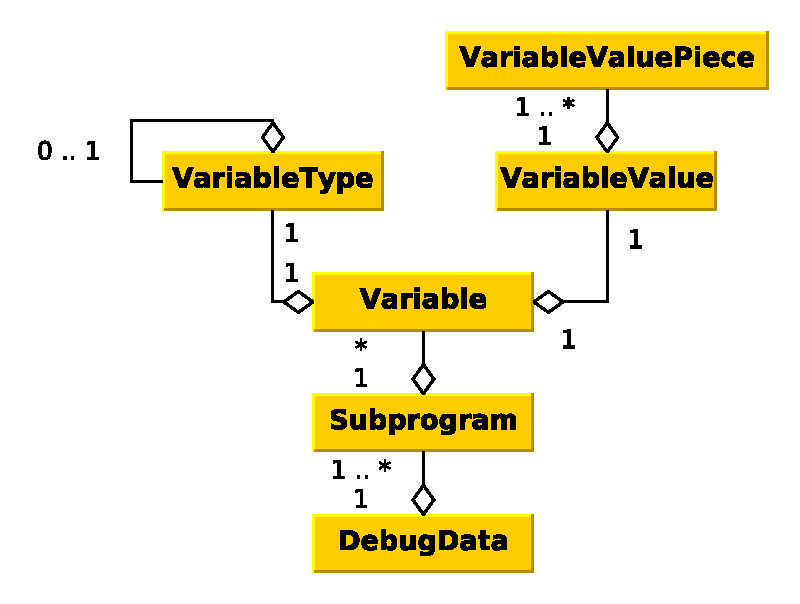
\includegraphics[trim=0cm 0cm 0cm 0cm, scale=0.7]{fig/dwarf_impl}
\caption{Diagram tříd reprezentujících DWARF struktury.}
\label{fig:dwarf_classes}
\end{figure}

\begin{itemize}
\item \textbf{VariableType} - Třída reprezentující typ proměnné uložené v DWARF informacích. Obsahuje informace jako je například název typu ("int", "char *", ...), velikost typu v bytech, způsob zakódování v paměti nebo například podtyp (v případě že jde o pole prvků jiného typu).
\item \textbf{VariableValuePiece} - Třída obsahující informaci o umístění části hodnoty proměnné v paměti nebo registrech mikrokontroleru. Hodnoty proměnných mohou být rozděleny na části například v případě, kdy část hodnoty proměnné je umístěna v registrech a část v paměti.
\item \textbf{VariableValue} - Pole instancí tříd VariableValuePiece, které reprezentuje kompletní hodnotu dané proměnné.
\item \textbf{Variable} - Třída zapouzdřující třídy VariableType a VariableValue definující jednu proměnnou daného programu.
\item \textbf{Subprogram} - Třída definující podprogram. Obsahuje seznam lokálních proměnných a argumentů podprogramu (instancí tříd Variable), jeho jméno a rozsah paměti, na které se kód podprogramu nachází
\item \textbf{DebugData} - Hlavní třída reprezentující kompletní DWARF ladící informace daného programu. Obsahuje seznam všech podprogramů (instancí tříd Subprogram).
\end{itemize}

Tyto třídy jsou obecnými třídami pro uchování ladících informací a nejsou nikterak přímo závislé na využítí formátu DWARF. V rámci této diplomové práce je však zpracováván pouze formát DWARF. Pro uložení dalších potřebných informací specifických pro formát DWARF bylo potřeba definovat ještě následující 3 třídy:

\begin{itemize}
\item \textbf{DwarfExpression} - Třída obsahující kód mikroinstrukcí pro zásobníkový automat definovaný formátem DWARF pro získání hodnoty proměnné (nebo její adresy) v závislosti na aktuálně zpracovávané instrukci. Tato třída zmíněný zásobníkový automat rovněž implementuje.
\item \textbf{DwarfLocation} - Třída zapouzdřující třídu DwarfExpression a definující rozsah adres, pro který je kód uložený v DwarfExpression platný.
\item \textbf{DwarfLocationList} - Seznam instancí tříd DwarfLocation.
\end{itemize}

Načtení DWARF ladících informací probíha za pomocí třídy DWARFLoader. Tato třída využívá nástroje objdump dodávaného s překladačem GCC. Nástroj objdump je postupně spuštěn s přepínači "--dwarf=info" a "--dwarf=loc", jejichž výstup je touto třídou rozparsován a zpracován a jsou vytvořeny instance výše zmíněných tříd.

\subsection{Využití DWARF informací}

Jedním z příkladu využití DWARF ladících informací je zobrazení lokálních proměnných aktuálně prováděného podprogramu. Při zastavení simulace na určité instrukci je za pomocí její adresy (hodnoty registru PC) nalezen aktuálně prováděný podprogram prostřednictvím třídy DebugData. Z podprogramu (instance třídy Subprogram) je získán seznam lokálních proměnných a pro každou proměnnou (instanci třídy Variable) je zavolána funkce pro získání její hodnoty.

Pokud není hodnota proměnné závislá na hodnotě registru PC, obsahuje instance třídy Variable přímo instanci třídy DwarfExpression. V opačném případě je v seznamu lokací DwarfLocationList nalezena odpovídající instance třídy DwarfExpression (na základě hodnoty registru PC). Dále je vyhodnocen kód zásobníkového automatu uloženého ve zmíněné třídě DwarfExpression a na základě výsledku je určena hodnota proměnné.

Hodnotu proměnné je potřeba reprezentovat odpovídajícím způsobem v závislosti na jejím typu. K tomu slouží třída VariableFormatter, která na základě typu proměnné formátuje její hodnotu a vrátí ji jako řetětec znaků.

\section{Knihovna simulující MCU MSP430}

Knihovna simulující MCU MSP430 vykonává instrukce simulovaného programu a implementuje interní moduly poskytované mikrokontrolerem.

Hlavní třídou knihovny je třída MCU\_MSP430, která reprezentuje celý mikrokontroler. V této třídě jsou vytvářeny a navzájem propojeny jednotlivé dílčí podtřídy, kterými se dále tato kapitola zabývá. Třída MCU\_MSP430 dědí ze třídy MCU a lze ji tak přímo použít jako rozšiřující modul simulátoru.

Nejjednoduššími třídami mikrokontroleru jsou třídy Memory, RegisterSet a Register. Třída Memory implementuje paměť jako pole bytů a umožňuje její čtení a zápis včetně informování o změně jednotlivých bytů pomocí instance třídy MemoryWatcher. Obdobně jsou implementovány třídy RegisterSet a Register.

\subsection{Implementace jednotlivých variant MCU MSP430}

Implementace knihovny umožňuje simulování většiny podporovaných variant mikrokontroleru MSP430. Každá varianta mikrokontroleru MSP430 je reprezentována vlastní třídou dědící ze třídy Variant. Tyto třídy jsou vytvořeny při načtení knihovny a lze k nim přistupovat na základě řetězce udávajícího název varianty funkcí getVariant(...).

Třída Variant obsahuje metody pro získání informací, které jsou pro dané varianty specifické. Jedná se například o adresy jednotlivých portů (metoda getP1DIR()), indexy vektorů přerušení (například metoda getUSART1TX\_VECTOR()) nebo například získání počáteční adresy vektoru přerušení (metoda getINTVECT()).

Vytváření těchto tříd ručně podle dokumentace by bylo značně obtížné a byl proto zvolen lepší přístup. Kompilátor msp430gcc obsahuje pro každou variantu mikrokontroleru hlavičkový soubor definující jednotlivé údaje a vlastnosti specifické pro daný mikrokontroler. Byl vytvořen skript v jazyce Python, kterým lze za použití nástroje msp430-gcc s přepínači -E a -dM získat z tohoto hlavičkového souboru seznam všech těchto definic pro daný mikrokontroler.

Tento seznam je pak dále zpracován a jsou z něj vybrány pouze ty definice, které jsou v knihovně simulující MCU MSP430 potřeba. Následně je vygenerována samotná třída Variant a i všechny její implementace - pro každý mikrokontroler jedna.

Tímto postupem byla jednoduše vyřešena většina rozdílů mezi variantami mikrokontrolerů včetně detekce různých interních modulů poskytovaných různými variantami.

\subsection{Načítání programu}

Pomocí knihovny lze načítat programy pro miktrokontroler ve formátu ELF a Intel HEX (A43). Načítání souborů ve formátu A43 provádí metoda loadA43(...) třídy Memory. Tato metoda rozparsuje data ve formátu A43, uloží je na dané místo v paměti a nastaví registr PC na adresu první instrukce.

Načítání souborů ve formátu ELF probíhá s využitím pomocné třídy CodeUtil. Ta za pomocí nástroje msp430-objcopy převede program z formátu ELF do formátu A43, který je pak možné načíst pomocí třídy Memory.

Při načítání programu je program rovněž disassemblován. To je provedeno pomocí nástroje msp430-objdump, jehož výstup je rozparsován a dále zpracováván grafickým uživatelským rozhraním.

\subsection{Dekódování a vykonávání instrukcí}

Instrukce je reprezentována instancí třídy Instruction. Tato třída uchovává informace o zdrojovém a cílovem argumentu instrukce, o jejím typu, offsetu a případném bytovém módu. Každý argument je uložen jako implementace abstraktní třídy InstructionArgument definující základní rozhraní argumentu. Byly implementovány následující typy argumentů:

\begin{itemize}
\item \textbf{ConstantArgument} - Argumentem je konstanta.
\item \textbf{MemoryArgument} - Argumentem je místo v paměti dané adresou.
\item \textbf{IndexedArgument} - Argumentem je místo v paměti dané adresou a offsetem.
\item \textbf{IndirectAutoincrementArgument} - Argumentem je místo v paměti dané adresou uloženou v registru, která je po vykonání instrukce inkrementována.
\item \textbf{Register} - Registr může být také argumentem instrukce a tak již dříve zmíněná třída Register rovněž implementuje třídu InstructionArgument.
\end{itemize}

Instrukce jsou dekódovány pomocí třídy InstructionDecoder. Tato třída načte aktuální instrukci z paměti, rozparsuje ji, uloží do instance třídy Instruction a vrací počet hodinových cyklů potřebných k těmto úkonům. Ke každému typu instrukce je definována funkce, která simuluje její vykonání. Tato funkce jako své parametry přijímá ukazatel na paměť (třídu Memory), registry (třídu RegisterSet) a aktuální instrukci (třídu Instruction). Návratovou hodnotou této funkce je rovněž počet hodinových cyklů potřebných k jejímu provedení.

Ukazatele na tyto funkce (indexované podle operačního kódu a typu instrukce) jsou uloženy ve tříde InstructionManager. Tato třída obsahuje metodu executeInstruction(...), která na základě typu a operačního kódu aktuální instrukce tuto instrukci vykoná (spustí příslušnou funkci včetně inkrementace PC registru).

Z pohledu simulace probíhá dekódování a vykonávání instrukcí ve třídě MCU\_MSP430, konkrétně v její metodě tickRising(...). Tato metoda je zprostředkovaně (za pomocí hodinového modulu) volána simulačním jádrem s každým cyklem MCLK hodin. S ohledem na počet hodinových cyklů potřebných k dekódování a vykonání instrukcí jsou pak instrukce postupně zpracovávány.

\subsection{Implementace pouzdra a pinů mikrokontroleru}

Mikrokontroler MSP430 na svém pouzdru obsahuje piny, ke kterým jsou uvnitř mikrokontroleru připojeny jednotlivé interní periferie. Je potřeba zajistit směrování signálů na správnou interní periferii a umožnit každé variantě mikrokontroleru definovat své vlastní pouzdrou.

\subsubsection{Pouzdro mikrokontroleru}

Pro uložení informace o pouzdru mikrokontroleru a možných pinech a jejich interních propojeních byl zvolen XML formát. Pro každou podporovanou variantu mikrokontroleru je k dispozici XML soubor v následujícím formátu:
\lstset{language=XML, numbers=left, frame=single, breaklines=true, tabsize=2, xleftmargin=20pt, literate=%
    {á}{{\'a}}1
    {č}{{\v{c}}}1
    {ď}{{\v{d}}}1
    {é}{{\'e}}1
    {ě}{{\v{e}}}1
    {í}{{\'i}}1
    {ň}{{\v{n}}}1
    {ó}{{\'o}}1
    {ř}{{\v{r}}}1
    {š}{{\v{s}}}1
    {ť}{{\v{t}}}1
    {ú}{{\'u}}1
    {ů}{{\r{u}}}1
    {ý}{{\'y}}1
    {ž}{{\v{z}}}1
    {Á}{{\'A}}1
    {Č}{{\v{C}}}1
    {Ď}{{\v{D}}}1
    {É}{{\'E}}1
    {Ě}{{\v{E}}}1
    {Í}{{\'I}}1
    {Ň}{{\v{N}}}1
    {Ó}{{\'O}}1
    {Ř}{{\v{R}}}1
    {Š}{{\v{S}}}1
    {Ť}{{\v{T}}}1
    {Ú}{{\'U}}1
    {Ů}{{\r{U}}}1
    {Ý}{{\'Y}}1
    {Ž}{{\v{Z}}}1}
\begin{lstlisting}
<variant>
<package name="MSP430x11x">
	<left>
		...
		<pin id="8">
			<name sel="0">P2.0</name>
			<name>ACLK</name>
		</pin>
		...
	</left>
	<right>
		...
		<pin id="13">
			<name sel="0">P1.0</name>
			<name dir="1" sel="1">TACLK</name>
			<name dir="0" sel="1">TACLK</name>
		</pin>
		...
	</right>
</package>
</variant>
\end{lstlisting}

Uvnitř elementu "package" se nachází definice pouzdra jedné varianty mikrokontroleru. Jednotlivé piny pouzdra jsou členěny podle strany pouzdra na které jsou umístěny: "left", "down", "right", "up". V těchto elementech se pak nachází samotné definice pinů. Každý pin má své id korespondující s číslováním pinu na pouzdru.

Jelikož může být k jednomu pinu připojeno více interních periferíí, má pin více jmen (element "name"). Aktuální jméno (a tím pádem i aktuální interní periferie připojená k pinu) je dáno konfigurací řídících registrů daného pinu. Typicky se jedná o PxDIR, PxSEL a PxSEL2. Element "name" umožňuje definovat hodnoty bitů těchto registrů odpovídající danému pinu pomocí atributů "sel", "dir" a "sel2". Tyto informace jsou pak využívány při mapování pinů na interní periferie.

Při vybrání konkrétní varianty mikrokontroleru MSP430 je načteno jeho pouzdrou pomocí třídy Package, která tento XML soubor zpracuje a vytvoří struktury potřebné k jeho vykreslení třídou MCU\_MSP430.

\subsubsection{Směrování signálů}

Pro každý pin načtený třídou Package je vytvořena instance třídy PinMultiplexer. Tato třída obsahuje seznam jmen všech interních periferií mapovaných na tento pin včetně podmínek určujících, kdy je která interní periferie aktivní. Třída PinMultiplexer obsahuje také seznam jmen všech interních periferií, kde ke každému jménu je přiřazena instance třídy PinHandler.

V případě změny řídícího registru (například PxSEL), jsou znovy vyhodnoceny podmínky uložené v instanci třídy PinMultiplexer a pokud došlo ke změně aktivní interní periferie, jsou všechny následující vstupní signály směrovány na nově aktivovanou interní periferii (reprezentovanou instancí třídy PinHandler).

Všechny instance třídy PinMultiplexer jsou spravovány třídou PinManager. Tato třída zpracovává veškeré vstupní signály mikrokontroleru MSP430, které mu předává simulační jádro. Pro každý vstupní signál je znám index pinu na který signál dorazil. Třída PinManager tak vyhledá instanci třídy PinMultiplexer tohoto pinu a zavolá její metodu handlePinInput(...), čímž přesune zpracování události na konrétní pin. Ten jej pak jen předá na aktivní instanci třídy PinHandler konkrétní interní periferii.

Při generování signálů je postup podobný. Interní periferie zavolá metodu generateOutput(...) třídy PinMultiplexer. Tato metoda ověří, zda-li je interní periferie aktivní pro daný pin. Pokud je aktivní, zavolá metodu generateOutput(...) třídy PinManager, která signál umístí na výstup kde jej přebere simulační jádro.

\subsubsection{Interní signály}

V rámci mikrokontroleru MSP430 existují i signály mezi interními periferiemi, které nejsou vyvedeny na piny na pouzdru. Pro reprezentaci a směrování těchto signálů slouží třída SignalManager. Jedná se třídu, pomocí které si může libovolná interní periferie zaregistrovat jméno signálu, který pak v budoucnu generuje. Ostatní periferie se mohou zaregistrovat k přijímání tohoto signálu.

\subsection{Implementace přerušení}

Při vzniku přerušení dojde po aktuální instrukci k zavolání rutiny přerušení definované adresou ve vektoru přerušení. Správa přerušení je v rámci knihovny simulující mikrokontroler MSP430 implementována ve třídě InterruptManager.

Interní periferie využívají k vygenerování přerušení metodu queueInterrupt(...). Tato metoda naplánuje nové přerušení. Jakmile dojde k dokončení simulace aktuální instrukce třídou MCU\_MSP430, zavolá tato třída metodu runQueuedInterrupts() třídy InterruptManager. Tato metoda přeruší aktuální program a spustí vykonávání rutiny přerušení s nejvyšší prioritou.

Interní periferie mohou implementovat třídu InterruptWatcher a být tak informovány o návratu z rutiny přerušení.

\subsection{Hodinový modul}

Hodinový modul umožňuje časování instrukcí a dalších interních periferií. Třídy hodinového modulu jsou v závislosti na své funkci (a jejich otcovské třídě) rozděleny do následujících skupin:

\begin{itemize}
\item \textbf{Oscilátory} - Skupina tříd dědících třídu Oscillator. Tyto třídy poskytují zdroj hodinového signálu další skupině tříd a jako jediné komunikují přímo s knihovnou ADEVS. Jedná se například o oscilátory LFXT1, VLO, XT2 nebo DCO.
\item \textbf{Hodiny} - Skupina tříd dědících třídu Clock. Tyto třídy využívají Oscilátory jako zdroj svého signálu (a většinou umožňují přepínat v závislosti na svých registrech mezi více oscilátory). Jedná se například o hodiny MCLK, SMCLK nebo ACLK.
\item \textbf{Časovač} - Třída reprezentující jeden časovač (například TimerA)  mikrokontroleru MSP430.
\end{itemize}

\subsubsection{Oscilátory}

Základem oscilátorů je již zmíněná třída Oscillator. Tato třída definuje základní rozhraní oscilátoru. Jedná se zejména o možnost zaregistrování instancí tříd OscillatorHandler, jejichž metody tickRising() a tickFalling() jsou volány při náběžné a sestupné hraně signálu. Třída Oscillator sama o sobě neposkytuje zdroj signálu, ale očekává, že bude ve správných intervalech volána její metoda tick().

V případě, že dojde k odebrání všech instancí tříd OscillatorHandler, je oscilátor pozastaven zavoláním metody pause(). Tím se zabrání zbytečnému tikání oscilátoru, který aktuálně není k ničemu potřeba. Při opětovném zaregistrování instance třídy OscillatorHandler je funkce oscilátoru znovu obnovena metodou start().

Třídy VLO a DCO rozšiřující třídu Oscillator implementují shodně pojmenované MSP430 oscilátory. Tyto třídy dědí rovněž třídu SimulationObject a chovají se jako samostatné simulační jednotky. Podle aktuálně nastavené frekvence naplánují svůj interní přechod za použití knihovny ADEVS v pevně stanovených intervalech. V tomto interním přechodu pak volají metodu tick(), čímž simulují pravidelné tikání oscilátoru.

Třídy LFXT1 a XT2 rovněž implementují třídu Oscillator a volají její metodu tick(). Volání této metody však neprobíhá na základě předem stanovené frekvence, ale podle změn signálu odpovídajících vstupních pinů. Tyto dva oscilátory tak nepoužívaji knihovnu ADEVS přímo, ale implementují třídu PinHandler a s její pomocí jsou napojeny na vstupní piny mikrokontroleru.

\subsubsection{Hodiny}

Základní třídou hodin je třída Clock. Tato třída plní stejnou funkci jako třída Oscillator pro oscilátory - definuje jejich základní rozhraní, umožňuje registrování instancí třídy ClockHandler a umožňuje volání jejich metod pomocí svých metod callRisingHandlers() a callFallingHandlers().

Třídu Clock dědí třídy ACLK, MCLK a SMCLK reprezentující stejnojmenné hodiny mikrokontroleru MSP430. Tyto třídy rovněž implementují třídu OscillatorHandler a na základě hodnoty svých řídicích registrů umožňují nastavovat zdrojový oscilátor a jeho děličku. Při každém tiku hodin jsou zavolány metody zaregistrovaných instancí tříd ClockHandler, které pak dále na hodinový signál reagují.

\subsubsection{Časovač}

Poslední částí hodinového modulu je Časovač. Jedná se o interní periferii implementující třídy ClockHandler, MemoryWatcher, InterruptWatcher a PinHandler. Tato periferie tak reaguje na hodinový signál, změny hodnot na určitých adresách v paměti, ukončení přerušení, vstupní signály a rovněž umožňuje generování výstupních signálů.


\subsection{Komunikační moduly}

Komunikační moduly umožňují komunikaci mikrokontroleru s jinými zařízeními. Jak již bylo zmíněno, v rámci této diplomové práce byla implementována pouze komunikace v módu SPI, avšak byla implementována v rámci všech tří komunikačních modulů - USI, USCI a USART.

Jednotlivé moduly jsou velmi obsáhlé, ale princip jejich tvorby se nelišil od časovače. Každý modul je tvořen jednou třídou implementující třídy ClockHandler, MemoryWatcher, InterruptWatcher, PinHandler a SignalHandler. Za pomocí těchto tříd komunikuje modul s ostatními částmi knihovny a implementuje nad nimi své chování.

Jelikož je potřeba vytvářet komunikační moduly v závislosti na variantě daného mikrokontroleru, existuje ke každé třídě modulu ještě pomocná třída, která vytvoří správný počet instancí daného modulu v závislosti na datech z aktuální instance třídy Variant.

\subsection{Automatické testování}

Knihovna simulující MCU MSP430 je jako jediná z celého simulátoru pokryta sadou automatických testů. Jedná se o sadu celkem 56 testů testujících jednotlivé části knihovny.

Pro implementaci testů je použita knihovna CPPUnit. Každá testovaná třída z knihovny má svoji odpovídající CPPUnit třídu, která ji testuje. Testování probíhá jak na základě znalostí vnitřní architektury knihovny (white box), tak pouze na základě vstupního programu a sledování reakcí knihovny na tento program (black box).

První třída testů většinou testuje konkrétni metody daných tříd knihovny. Jako příklad lze uvést testy dekódování instrukcí, testy pamětí a registrů nebo například test směrování signálů mezi piny.

Druhá třída testů pak funguje tak, že je do paměti nahrán konkrétní program pro daný mikrokontroler a v rámci testu je instrukci po instrukci vykonáván. Vždy se testuje, zda hodnoty registrů odpovídají očekávání a zda instrukce vykonala danou operaci. Z této třídy testů lze zmínit test BlinkingLed testující program blikající LED diody, nebo test Capture testující zachytávání signálu časovačem.

\section{Grafické uživatelské rozhraní}

Grafické uživatelské rozhraní (GUI) je naprogramováno v jazyce C++ za použití knihovny Qt a umožňuje řízení celé simulace. V této podkapitole je popsána implementace dílčích částí GUI a jejich návaznost na další části simulátoru popsané v předešlých podkapitolách.

\subsection{Hlavní okno}

Základní třídou celé aplikace je třída QSimKit reprezentující její hlavní okno. Tato třída vytváří a zapouzdřuje všechny další části GUI popsané dále v této části diplomové práce.

Hlavní okno aplikace lze vidět na obrázku \ref{fig:screen}. Na horní části okna jsou ovládácí prvky určené k řízení simulace a nastavení velikosti kroku při jejím krokování. Ve středu okna se nachází kreslící plocha popsaná v podkapitole \ref{kreslici_plocha}. V levé části okna jsou zobrazeny detaily periferií a mikrokontroleru (podkapitola \ref{detaily_per}). Pravá část okna zobrazuje aktuální program běžící uvnitř mikrokontroleru (podkapitopla \ref{screen_disassembler}) a ve spodní části okna lze formou osciloskopu sledovat jednotlivé piny (podkapitola \ref{screen_tracking}).

\begin{figure}[ht]
\centering
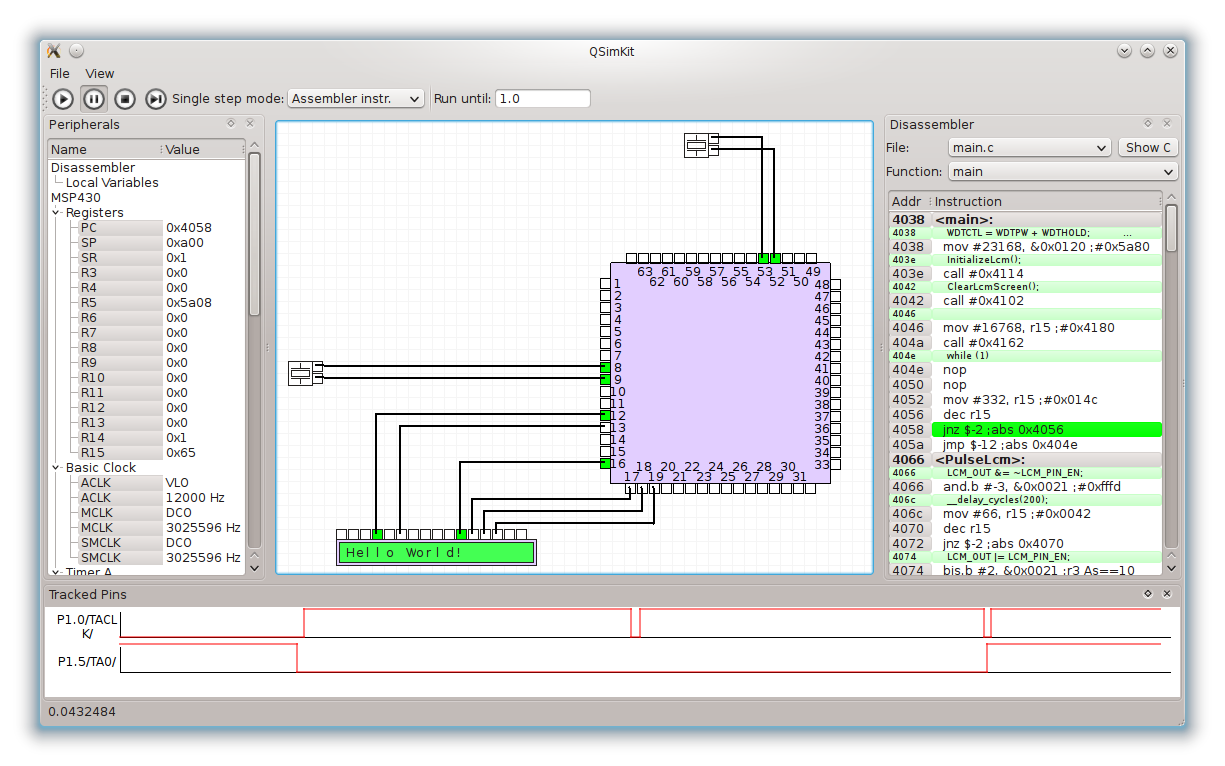
\includegraphics[trim=0cm 0cm 0cm 0cm, scale=0.45]{fig/screen}
\caption{Hlavní okno grafického uživatelského rozhraní.}
\label{fig:screen}
\end{figure}

\subsection{Kreslící plocha}
\label{kreslici_plocha}

Kreslící plocha zobrazuje MCU a jednotlivé periferie včetně jejich propojení. Umožňuje přidání nových periferí, odebrání stávajících a jejich propojování.

Každá periferie zobrazená na kreslící ploše je dceřinou třídou třídy ScreenObject. Tato třída obsahuje základní informace o každém objektu, jako jsou jeho umístění, velikost, jména a umístění jeho pinů nebo například seznam akcí zobrazených v kontextovém menu objektu. Obsahuje také funkci paint(...), která slouží k vykreslení objektu na daných souřadnicích.

Samotné vykreslení kreslící plochy a správa jejich objektů probíha ve třídě Screen rozšiřující třídy QWidget. Ta obsahuje seznam všech instancí třídy ScreenObject, provádí jejich vykreslení a umožňuje jejich posouvání, přidávání a odstraňování. Při spuštění simulace je zavolána její metoda prepareSimulation(...), která ke každému objektu typu ScreenObject vytvoří odpovídající objekt typu SimulationObjectWrapper a přidá jej do aktuální simulace. V průběhu simulace je kreslící plocha periodicky vykreslována.

\subsubsection{Propojování pinů}

Propojování pinů jednotlivých periferií probíhá ve třídě ConnectionManager. Této třídě jsou třídou Screen předány Qt události potřebné k vytváření nových propojení. Třída Screen rovněž volá metodu paint(...) třídy ConnectionManager pro vykreslení propojení pinů. Jednotlivá propojení jsou uložena v seznamu struktur typu Connection. Každá položka seznamu obsahuje ukazatel na objekt a pin ze kterého propojení vychází a objekt a pin do kterého spojení vstupuje. Jsou zde také uloženy souřadnice klíčových bodů na kreslící ploše, kterými propojení prochází.

Třída ConnectionManager obsahuje, podobně jako třída Screen, metodu prepareSimulation(...). Tato metoda propojí jednotlivé piny objektů typu SimulationObjectWrapper při spuštění simulace a zařídí tak správné směrování simulačních událostí.

Lze také vytvořit propojení více než dvou objektů. V tomto případě je na kreslící plochu přidán nový objekt typu ConnectionNode. Tento objekt má 4 piny (na každé ze svých stran jeden) a při simulování přenáší veškeré přijaté signály z libovolného pinu na všechny své piny.

\subsubsection{Přidání nové periferie na kreslící plochu}

Pro přidání nové periferi na kreslící plochu slouží dialogové okno AddPeripheral (viz obrázek \ref{fig:addperipheral}) vyvolané pomocí kontextového menu kreslící plochy. Toto dialogové okno prostřednictvím instance třídy PeripheralManager získá seznam všech dostupných periferií a umožní uživateli jejich výběr. Tento dialog také zobrazuje náhled periferie za pomocí třídy ScreenObjectPreview. Tato třída vytváří novou dočasnou instanci periferie a vykreslí ji.

\begin{figure}[ht]
\centering
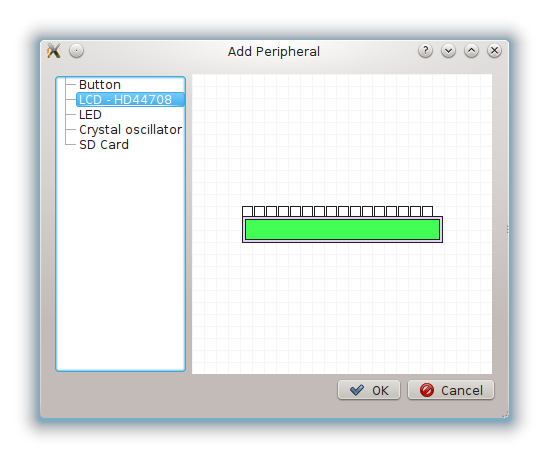
\includegraphics[trim=0cm 0cm 0cm 0cm]{fig/addperipheral}
\caption{Dialog pro přidání nové periferie.}
\label{fig:addperipheral}
\end{figure}

\subsection{Detaily periferií a mikrokontroleru}
\label{detaily_per}

Detaily jednotlivých periferií a mikrokontroleru lze vidět v levé části hlavního okna. Základem je třída Peripherals obsahující seznam všech položek jednotlivých periferií uložených a zobrazených pomocí Qt třídy QTreeWidget. Při přidání nebo odebrání nové periferie je zavolána její metoda getPeripheralItem(...), která vrátí položku periferie (instanci třídy PeripheralItem) reprezentující tuto periferii v seznamu periferií.

Každá periferie tak může implementovat vlastní implementaci třídy PeripheralItem, která je pak v detailech periferií zobrazena. Kromě obecné třídy PeripheralItem existují i další dvě třídy: MemoryItem a VariableItem.

Třída MemoryItem je využita pro položky zobrazující hodnotu místa v paměti mikrokontroleru. V případě přidání této položky do detailů periferií umožní třída Peripherals vytváření nových breakpointů na základě adresy periferie a automaticky zobrazuje za pomocí třídy VariableFormatter hodnotu adresové buňky ve správném formátu na základě jejího typu.

Třída VariableItem pak slouží k zobrazení hodnoty lokálních proměnných za pomocí DWARF ladících informací.

\subsection{Disassembler}
\label{screen_disassembler}

Disassembler slouží k zobrazení zdrojového kódu programu aktuálně zpracovávaného mikrokontrolerem. Hlavní třídou je třída Disassembler. Při pridání nového mikrokontroleru nebo změně jeho programu je znovu nahrán disassemblovaný kód a případné ladící informace. Zdrojový kód je zobrazen v Qt objektu typu QTreeWidget. V horní části disassembleru může uživatel vybrat zdrojový soubor programu a název funkce, kterou chce v tomto zdrojovém souboru zobrazit. Zobrazení zdrojového kódu lze přepínat mezi assemblerem a zdrojovým kódem v jazyce C.

Po přerušení simulace (nebo například krokování programu) je na základě hodnoty PC registru metodou pointToInstruction(...) zobrazena aktuální instrukce. Uživatel rovněž může pomocí kontextového menu přidávat nové breakpointy. Adresy instrukcí, na kterých je nastaven breakpoint jsou zobrazeny červenou barvou.

Diassembler rovněž přidává instanci třídy DisassemblerItem implementující třídu PeripheralItem do detailů periferií. Uživatel tak při krokování nebo přerušení simulace vidí v detailech periferí hodnoty lokálních proměnných v aktuální funkci.

\subsection{Sledování pinů}
\label{screen_tracking}

Sledování pinů (na obrázku simulátoru dole) je umožněno pomocí třídy TrackedPins. Tato třída je napojena na signály třídy Screen informující o změně sledovaných pinů (Sledování lze pro každý pin nastavit v jeho kontextovém menu na kreslící ploše). Pokud dojde ke změně sledovaných pinů, třídy TrackedPins přidá nebo odstraní tento pin z instance třídy Plot, kterou zapouzdřuje.

Třída Plot se stará o samotné vykreslení grafů zobrazujících změnu napětí na jednotlivých sledovaných pinech. Pro každý pin je uchováno jeho jméno a ukazatel na instanci třídy PinHistory, která obsahuje vykreslovaná data. Instance třídy PinHistory jsou vytvořeny a spravovány ve třídě SimulationObjectWrapper.

Pokud dojde k přeposlání simulační události třídou SimulationObjectWrapper a daný pin je sledován, je informace o této události vložena do odpovídající instance třídy PinHistory. Pokud je navíc výstup vygenerován zpracováním určité intrukce, je její adresa rovněž uložena a uživatel pak může pomocí kontextového menu zobrazit instrukci, která je zodpovědná za danou změnu v grafu.

Třída Plot rovněž umožňuje měnit měřítko grafu, označovat jeho úseky a zobrazuje délku označeného úseku v sekundách.

\subsection{Správa projektu}

Základní funkcí GUI je správa projektu. Jedná se zejména o jeho vytvoření, uložení a opětovné nahrání.

\subsubsection{Vytvoření projektu}

Bezprostředně po vytvoření nového projektu je zobrazen dialog ProjectConfiguration umožňující jeho konfiguraci. Tento dialog (viz obrázek \ref{fig:projectconf}) umožňuje výběr rodiny mikrokontrolerů pro projekt (aktuálně pouze MSP430) a výběr konkrétního modelu mikrokontroleru. Ve středu dialogu je zobrazena ukázka daného mikrokontroleru. Pomocí tlačítka "Show features" je možné zobrazit vlastnosti daného mikrokontroleru podporované simulátorem.

Po potvrzení dialogu je vybraný mikrokontroler vložen na kreslící plochu a lze s ním dále pracovat.

\begin{figure}[ht]
\centering
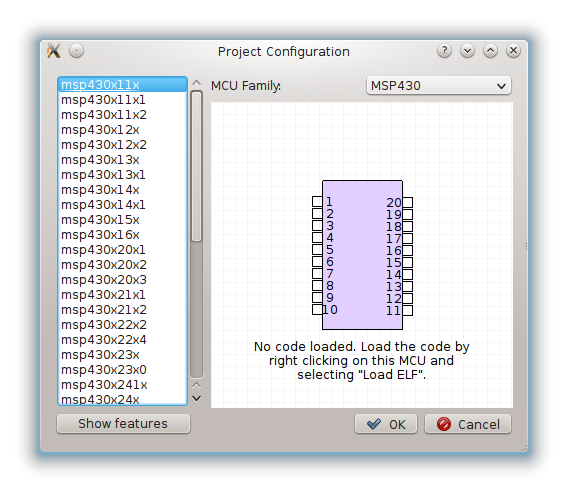
\includegraphics[trim=0cm 0cm 0cm 0cm, scale=0.7]{fig/projectconf}
\caption{Dialog pro konfiguraci projektu.}
\label{fig:projectconf}
\end{figure}

\subsubsection{Formát uložených projektů}

Projekt je možné uložit do souboru ve formátu XML s příponou "qsp" (QSimkit Project). Základní vnitřní členění tohoto souboru je následující:

\lstset{language=XML, numbers=left, frame=single, breaklines=true, tabsize=2, xleftmargin=20pt}
\begin{lstlisting}
<qsimkit_project>
	<objects>
		<object id='0' type='msp430' interface='mcu' name='MSP430'>
			<position x='192' y='60'/>
			<code> ... </code>
			<variant>msp430x16x</variant>
			<a43path> ... </a43path>
			<elfpath> ... </elfpath>
			<elf> ... </elf>
		</object>
	...
	</objects>
	<connections> ... </connections>
	<trackedpins> ... </trackedpins>
	<registerbreakpoints> ... </registerbreakpoints>
	<memorybreakpoints> ... </memorybreakpoints>
</qsimkit_project>
\end{lstlisting}

Kořenovým elementem je element "qsimkit\_project". Jeho vnitřní elementy pak mají následující význam:

\begin{itemize}
\item \textbf{objects} - Uchovává seznam všech objektů vytvořených v rámci projektu.
\begin{itemize}
\item \textbf{object} - Každý objekt má svůj typ, jméno a pozici. Každý objekt může kromě těchto základních informací ukládat i informace pro něj specifické. Například objekt s rozhraním typu "mcu" reprezentuje mikrokontroler a jako rozšiřující informace ukládá kód aktuálního programu a cestu k jeho zdroji.
\end{itemize}
\item \textbf{connections} - Ukládá propojení mezi objekty. O každém propojení jsou známy jeho uzlové body na kreslící ploše a objekty s jejich piny, které propojení spojuje.
\item \textbf{trackedpins} - Slouží pro uložení seznamu sledovaných pinů.
\item \textbf{registerbreakpoints} - Uchovává seznam všech bodů zastavení pro registry. 
\item \textbf{memorybreakpoints} - Analogicky k registerbreakpoints uchovává seznam všech bodů zastavení pro paměťové buňky.
\end{itemize}


\subsubsection{Uložení a nahrání projektu}

Uložení je iniciováno ze třídy QSimKit, která umožní uživateli výběr souboru pro uložení projektu, vytvoří QSP soubor a k němu odpovídající instanci třídy QTextStream. Ukládání dat do tohoto souboru pak provádí další třídy simulátoru. Třída Screen ve své metodě save(...) projde seznam všech svých objektů, uloží do souboru jejich základní informace a pro informace rozšiřující zavolá metodu save(...) každého objektu. V této metodě pak mají jednotlivé objekty možnost uložit pro ně specifické informace.

Obdobně je volána metoda save(...) třídy ConnectionManager ukládající informace o spojeních mezi objekty.

Nahrávání projektu probíhá analogicky s tím rozdílem, že jsou volány metody load(...) jednotlivých tříd, které z instance třídy QDomDocument získají potřebná data.

\subsection{Konzolový simulátor}

Součástí simulátoru je i konzolová (textová) aplikace umožňující načítat a simulovat projekty vytvořené v grafickém uživatelském rozhraní. Tato aplikace je určena především jako ukázka, jak využít simulační jádro bez grafického uživatelského rozhraní. Výhodou je rychlejší běh simulace, protože není potřeba aktualizovat během simulace kreslící plochu a reagovat na vstupy uživatele.

\section{Rozšiřující moduly}

V rámci diplomové práce bylo implementováno celkem pět rozšiřujících modulů. V této podkapitole jsou jednotlivé moduly stručně popsány. Jedná se o moduly implementující tlačítko, LED diodu, LCD displej, oscilátor a SD kartu.

Moduly tlačítka a oscilátoru jsou rozebrány podrobněji také v případové studii v rámci kapitoly \ref{pripad}.

\subsection{Tlačítko}

Modul tlačitka (viz obrázek \ref{fig:tlacitko}) implementuje jednoduché tlačítko v jazyce Python. Po kliknutí na něj změní tlačítko svůj stav a vygeneruje odpovídající napětí na svůj výstupní pin. Uživateli je umožněno vybrat, bude-li tlačítko generovat v sepnutém stavu logickou 1 nebo 0.

\begin{figure}[ht]
\centering
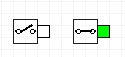
\includegraphics[trim=0cm 0cm 0cm 0cm, scale=1]{fig/button}
\caption{Nesepnutý a sepnutý stav tlačítka.}
\label{fig:tlacitko}
\end{figure}

\subsection{LED dioda}

Modul LED diody (lze vidět na obrázku \ref{fig:dioda}) je rovněž implementován v jazyce Python. Jeho funkcí je při logické 1 na vstupu zobrazit rozsvícenou LED diodu. Uživatel může vybrat barvu diody pomocí jejího kontextového menu.

\begin{figure}[ht]
\centering
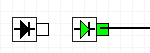
\includegraphics[trim=0cm 0cm 0cm 0cm, scale=1]{fig/led}
\caption{Nesvítící a svítící LED dioda.}
\label{fig:dioda}
\end{figure}

\subsection{LCD displej}

Modul LCD displeje (viz obrázek \ref{fig:lcd}) implementuje v jazyce Python LCD displej postavený na integrovaném obvodu HD44780 \cite{hd44780}. Nejedná se o kompletní implementaci tohoto integrovaného obvodu. Pro účely testování simulátoru byly implementovány pouze následující vlastnosti obvodu HD44780:

\begin{itemize}
\item Pouze 1 řádek, 16 alfanumerických znaků.
\item Řízení pomocí 4 nebo 8 vodičů.
\item Smazání displeje.
\item Přesunutí kurzoru na začátek.
\item Nastavení inkrementace (dekrementace) pozice kurzoru při nahrání znaku.
\end{itemize}

\begin{figure}[ht]
\centering
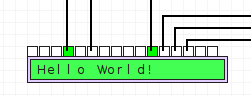
\includegraphics[trim=0cm 0cm 0cm 0cm, scale=1]{fig/lcd}
\caption{LCD displej zobrazující testovací text nahraný pomocí mikrokontroleru.}
\label{fig:lcd}
\end{figure}

\subsection{SD karta}

Modul SD karty (viz obrázek \ref{fig:sd}) vznikl zejména za účelem testování komunikačních modulů komunikujících pomocí SPI. Podobně jako modul LCD displeje je i modul SD karty naprogramován v jazyce Python a neimplementuje kompletní standard \cite{sdio} definující komunikační rozhraní SD karty.

\begin{figure}[ht]
\centering
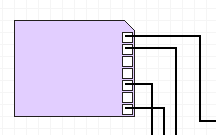
\includegraphics[trim=0cm 0cm 0cm 0cm, scale=1]{fig/sd}
\caption{Modul SD karty.}
\label{fig:sd}
\end{figure}

Implementace modulu je v rámci diplomové práce omezena na následující vlastnosti:

\begin{itemize}
\item Velikost SD karty pouze 2MB.
\item Čtení CSD dat SD karty - tato data popisují vlastnosti SD karty (například její velikost).
\item Možnost nastavit délku bloku čtených/zapisovaných dat.
\item Čtení a zápis dat na libovolnou adresu SD karty včetně blokového zápisu a čtení.
\end{itemize}

\subsection{Oscilátor}

Modul oscilátoru (viz obrázek \ref{fig:oscilator}) slouží ke generování periodického signálu. Uživatel může pomocí kontextového menu vybrat frekvenci tohoto signálu. Jako jediný z modulů je tento modul implementován v jazyce C++. Tento jazyk byl zvolen zejména kvůli nutnosti vyššího výkonu, protože oscilátor generuje nové události velmi často.

\begin{figure}[ht]
\centering
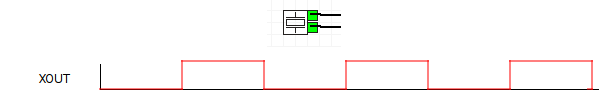
\includegraphics[trim=0cm 0cm 0cm 0cm, scale=0.8]{fig/oscilator}
\caption{Modul oscilátoru a ukázka signálu, který generuje.}
\label{fig:oscilator}
\end{figure}

\chapter{Ověření korektní funkce simulátoru}

V rámci této kapitoly je popsán postup ověření korektnosti simulátoru, jednotlivé testy a jejich výsledky. Cílem bylo převážně ověření časování funkcí mikrokontroleru a jeho výstupu. Vzhledem k využití automatických testů při implementaci knihovny simulující mikrokontroler MSP430 je právě časování jedinou neotestovanou částí simulátoru.

Testování probíhalo za použití zařízení FITKit verze 1.2 s mikrokontrolerem MSP430F168IPM. Do tohoto mikrokontroleru byly nahrávány testovací programy a výstup mikrokontroleru byl snímán dvoukanálovým osciloskopem 50MHz VELLEMAN F-KV-PCS500 SE \cite{velleman}. Následně byl stejný program spuštěn v simulátoru a za pomocí sledování pinů byly naměřeny hodnoty ze stejných pinů jako na reálném mikrokontroleru.

V dalších podkapitolách jsou jednotlivé testovací programy podrobněji rozebrány a okomentovány jejich výsledky.

\section{Ověření vztahu mezi instrukcemi a MCLK}
\label{test1}

Tento test byl zaměřen na ověření časování instrukcí a jejich návaznost na tikání MCLK hodin. Byl použit jednoduchý program, který nastaví počáteční frekvenci mikrokontroleru (registry BCSCTL1 a DCOCTL). Dále nastaví pin P1.4 jako výstupní a na jeho výstup zvolí hodinový signál SMCLK. Tento signál je standardně nastaven na stejnou frekvenci jako MCLK a lze jej tak považovat v rámci tohoto testu jako ekvivalentní MCLK. Výstup MCLK nemohl být použit přímo z důvodu konstrukce zařízení FITKit. Jako výstupní byl rovněž nastaven pin P1.7, na kterém pak ve smyčce program invertuje jeho hodnotu. Celý kód programu vypadal takto:

\lstset{language=XML, numbers=left, frame=single, breaklines=true, tabsize=2, xleftmargin=20pt}
\begin{lstlisting}
#include "msp430x16x.h"
int main(void) {
	WDTCTL = WDTPW + WDTHOLD;
	BCSCTL1 = ((BCSCTL1 & ~(0x0f)) | 7);
	DCOCTL  = ((DCOCTL & ~(0xe0)) | (3 << 5));
	P1DIR |= BIT7 | BIT4;
	P1SEL |= BIT4;
	for(;;) {
		P1OUT ^= BIT7;
	}
}
\end{lstlisting}

Osciloskop byl připojen k pinům P1.7 a P1.4. Cílem bylo změřit frekvenci mikrokontroleru, frekvenci invertování pinu P1.7 a počet tiků mikrokontroleru během jednoho invertování pinu P1.7. Výsledek měření lze vidět na obrázku \ref{fig:dso04osc}.

\begin{figure}[ht]
\centering
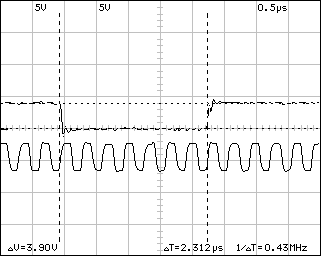
\includegraphics[trim=0cm 0cm 0cm 0cm, scale=1]{fig/dso04}
\caption{Naměřené hodnoty osciloskopem na reálném mikrokontroleru.}
\label{fig:dso04osc}
\end{figure}

Z výsledku je patrné, že délka setrvání pinu P1.7 v jednom stavu je 2.312 us. Během tohoto času dojde k 7 tikům mikrokontroleru. Perioda jednoho tiku je tak 0.33028 us, což odpovídá frekvenci mikrokontroleru 3.027 MHz.

Na obrázku \ref{fig:dso04sim} lze vidět výstup stejného programu běžícího v simulátoru.

\begin{figure}[ht]
\centering
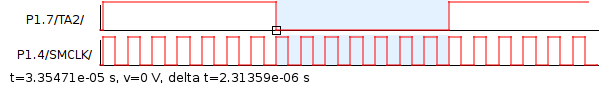
\includegraphics[trim=0cm 0cm 0cm 0cm, scale=0.8]{fig/dso04sim}
\caption{Naměřené hodnoty v simulátoru.}
\label{fig:dso04sim}
\end{figure}

V simulátoru setrval pin P1.7 v jednom stavu po dobu 2.31359 us. Rovněž došlo k sedmi tikům mikrokontroleru a perioda jednoho tiku je tak 0.33051 us. To odpovída frekvenci mikrokontroleru 3.025 Mhz.

Z porovnání výsledků lze vidět, že časování simulátoru je velmi blízké reálnému mikrokontroleru. Odchylka je způsobena zejména standardně využitým DCO oscilátorem, který může dosahovat na reálném mikrokontroleru větších nepřesností. Při použití přesného externího oscilátoru lze očekávat ještě přesnější výsledky.

\section{Ověření časování instrukcí}
\label{test2}

Tento test je podobný jako test předchozí, ale do hlavní smyčky programu byla vložena další čekací smyčka, která prodlužuje frekvenci invertování pinů. Cílem testu je ověřit časování instrukcí na delším časovém úseku. Pro vizuální kontrolu na zařízení FITKit je invertován rovněž pin P1.0 blikající červenou diodou.

Celý kód programu vypadal takto:

\lstset{language=XML, numbers=left, frame=single, breaklines=true, tabsize=2, xleftmargin=20pt}
\begin{lstlisting}
#include "msp430x16x.h"
int main(void) {
	volatile unsigned int i = DELAY;
	WDTCTL = WDTPW + WDTHOLD;
	BCSCTL1 = ((BCSCTL1 & ~(0x0f)) | 7);
	DCOCTL  = ((DCOCTL & ~(0xe0)) | (3 << 5));
	P1DIR |= BIT0 | BIT7;
	P1OUT = BIT0;
	for(;;) {
		i = 32000;
		P1OUT ^= BIT0;
		P1OUT ^= BIT7;
		do
			i--;
		while (i > 0);
	}
}
\end{lstlisting}

Osciloskop byl připojen pouze k pinu P1.7. Výsledek měření lze vidět na obrázku \ref{fig:dso05osc}.

\begin{figure}[ht]
\centering
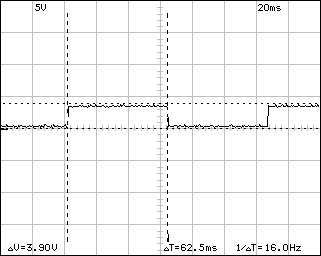
\includegraphics[trim=0cm 0cm 0cm 0cm]{fig/dso05}
\caption{Naměřené hodnoty osciloskopem na reálném mikrokontroleru.}
\label{fig:dso05osc}
\end{figure}

Doba setrvání pinu P1.7 v jednom stavu byla 62.5 ms. Výsledky stejného programu simulovaného v simulátoru lze vidět na obrázku \ref{fig:dso05sim}.

\begin{figure}[ht]
\centering
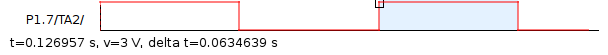
\includegraphics[trim=0cm 0cm 0cm 0cm, scale=0.8]{fig/dso05sim}
\caption{Naměřené hodnoty v simulátoru.}
\label{fig:dso05sim}
\end{figure}

Z porovnání výsledků opět vyplývá, že simulovaný program odpovídá programu na reálném mikrokontroleru. Drobná odchylka je způsobena rozdílnou frekvencí reálného mikrokontroleru. Ke zpřesnění by opět došlo při použití externího oscilátoru místo interního oscilátoru DCO.

\section{Ověření funkce časovače}
\label{test3}

Cílem tohoto testu bylo ověřit správnou funkci časovače za použití jednoduchého programu invertujícího periodicky výstupní pin P1.7. Program nastaví časovač na vyvolání přerušení při napočítání do 1260. Po pěti přerušeních je invertován pin P1.7.

Celý kód programu vypadal takto:

\lstset{language=XML, numbers=left, frame=single, breaklines=true, tabsize=2, xleftmargin=20pt}
\begin{lstlisting}
#include "msp430x16x.h"
#include <signal.h>
volatile unsigned int count = 0;
interrupt(TIMERA0_VECTOR) timer_interrupt(void) {
	if (++count == 5) {
		P1OUT ^= BIT7;
		count = 0;
	}
}

int main(void) {
	WDTCTL = (WDTPW + WDTHOLD);
	BCSCTL1 = ((BCSCTL1 & ~(0x0f)) | 7);
	DCOCTL  = ((DCOCTL & ~(0xe0)) | (3 << 5));
	TACTL |= (TASSEL_2 + ID_0 + TACLR);
	CCR0 = 1260;	CCTL0 = CCIE;
	TACTL |= MC_1; 	P1DIR |= BIT7;
	__enable_interrupt();
	while(1) {}
	return 0;
}

\end{lstlisting}

Osciloskop byl připojen pouze k pinu P1.7. Výsledek měření lze vidět na obrázku \ref{fig:dso06osc}.

\begin{figure}[ht]
\centering
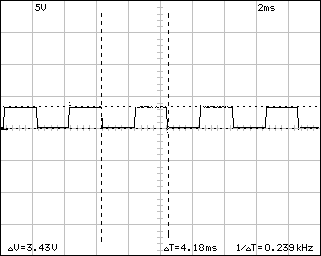
\includegraphics[trim=0cm 0cm 0cm 0cm]{fig/dso06}
\caption{Naměřené hodnoty osciloskopem na reálném mikrokontroleru.}
\label{fig:dso06osc}
\end{figure}

Doba setrvání pinu P1.7 v jednom stavu byla 4.18 ms. Výsledky stejného programu simulovaného v simulátoru lze vidět na obrázku \ref{fig:dso06sim}.

\begin{figure}[ht]
\centering
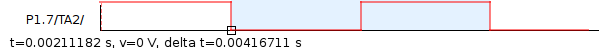
\includegraphics[trim=0cm 0cm 0cm 0cm, scale=0.8]{fig/dso06sim}
\caption{Naměřené hodnoty v simulátoru.}
\label{fig:dso06sim}
\end{figure}

V simulátoru byla naměřena hodnota 4.16 ms. Časování simulovaného programu tak odpovídá reálnému mikrokontroleru.

\section{Test rychlosti simulace}

V následující části jsou jednotlivé testy z předchozích podkapitol spuštěny znovu za účelem porovnání rychlosti simulace s reálným mikrokontrolerem.

Testy byly prováděny na notebooku s procesorem AMD Turion II P520 Dual-Core Processor o frekvenci 2300 MHz. Výsledkem testování jsou tabulky porovnávající délku simulace nutnou k odsimulování 500 ms běhu mikrokontroleru. Testy byly prováděny jak v grafickém uživatelském rozhraní tak v konzolovém simulátoru.

Obrázek \ref{fig:tabulka1} zobrazuje tabulku s výsledky rychlosti simulace na mikrokontroleru řady MSP430x16x o frekvenci 3 025 596 Hz. Test 1 až Test 3 v této tabulce koresponduje s programy v podkapitolách \ref{test1}, \ref{test2} a \ref{test3}.

\begin{figure}[ht]
\centering
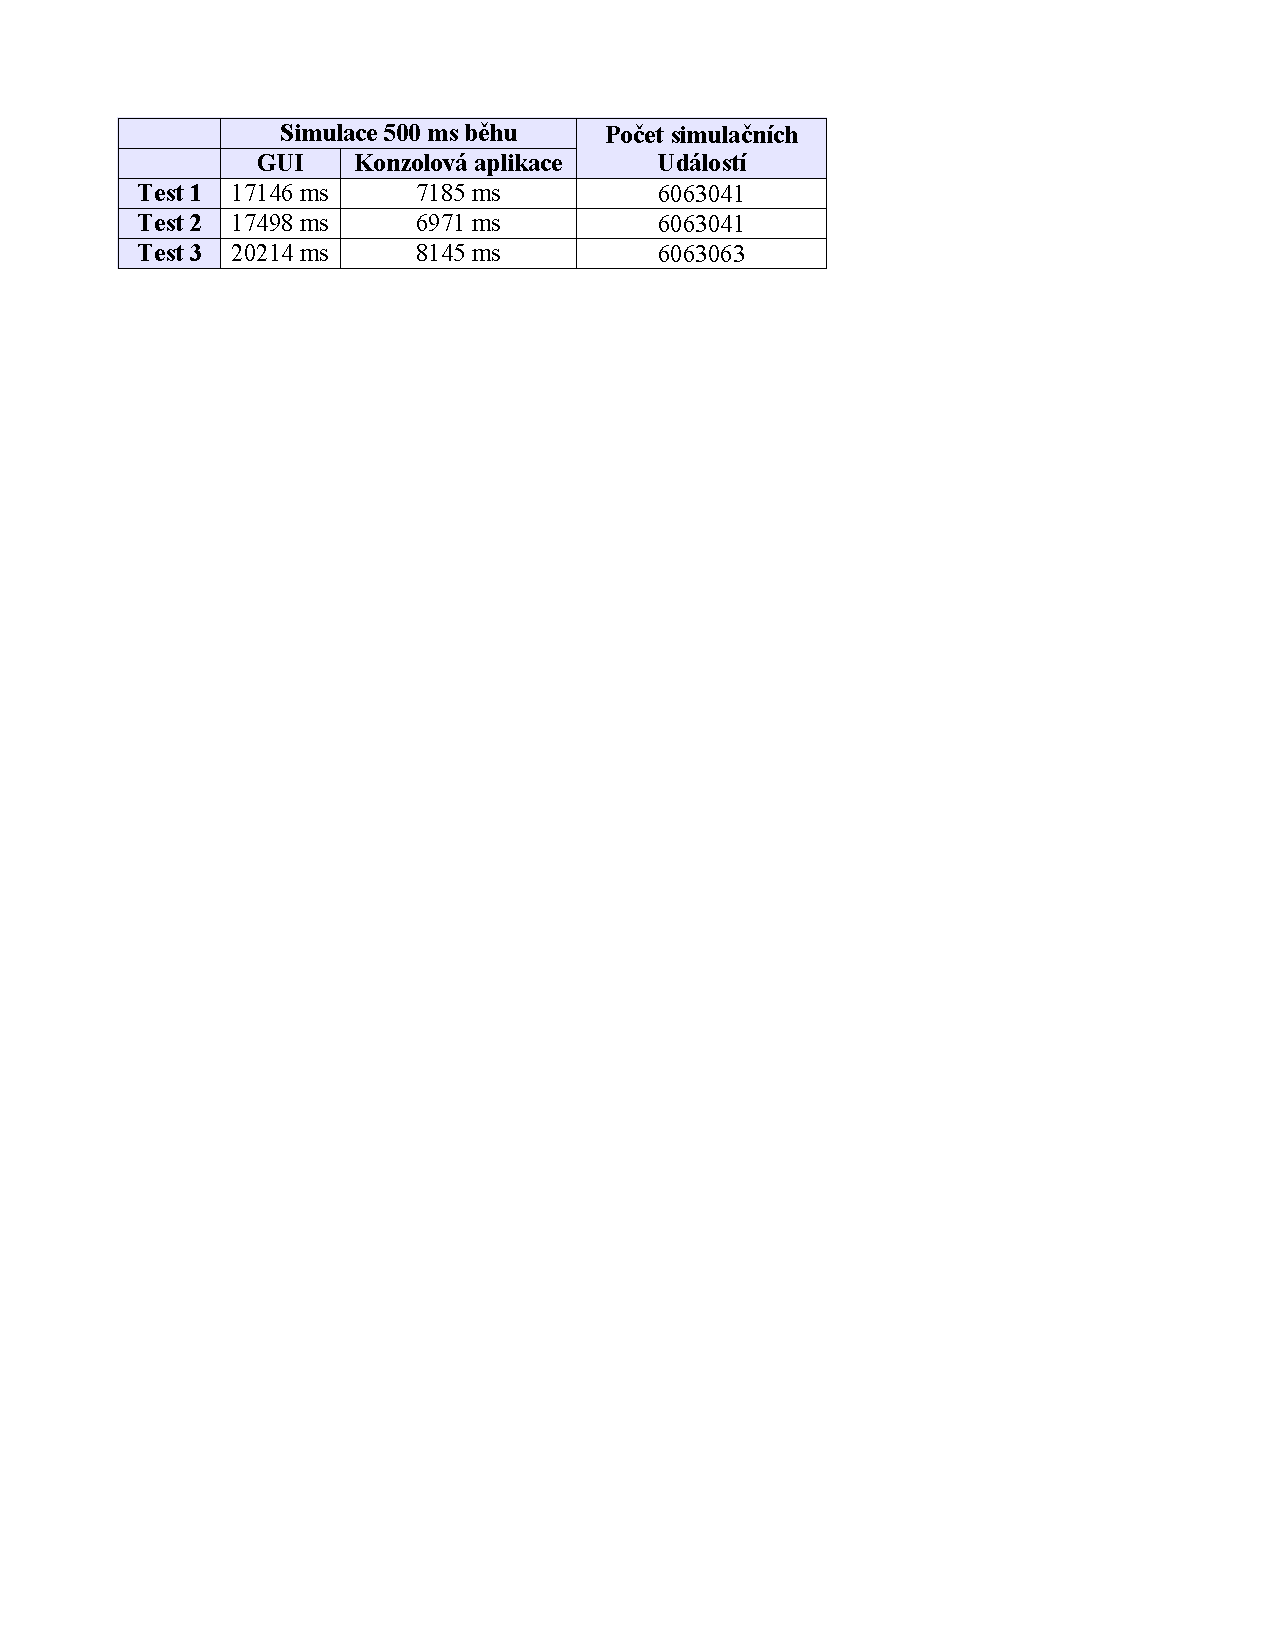
\includegraphics[trim=0cm 23.5cm 2cm 2cm]{fig/tabulka1}
\caption{Tabulka shrnující testy rychlosti simulace na mikrokontroleru řady MSP430x16x o frekvenci 3 025 596 Hz}
\label{fig:tabulka1}
\end{figure}

Jak lze z tabulky na první pohled vyčíst, je konzolová aplikace přibližně 2.38x rychlejší než stejná simulace v grafickém uživatelském rozhraní. To je způsobeno nutností aktualizace grafického uživatelského rozhraní v průběhu simulace.

Z tabulky rovněž vyplývá, že grafické uživatelské rozhraní zpracuje za sekundu 353612 simulačních událostí, zatímco konzolová aplikace jich zpracuje 843847. Dále je patrné, že Test 3 trval déle než ostatní testy. To je způsobeno běžícím časovačem v tomto testu, který generuje další simulační události, které je třeba obsloužit, což zabere další čas.

\begin{figure}[ht]
\centering
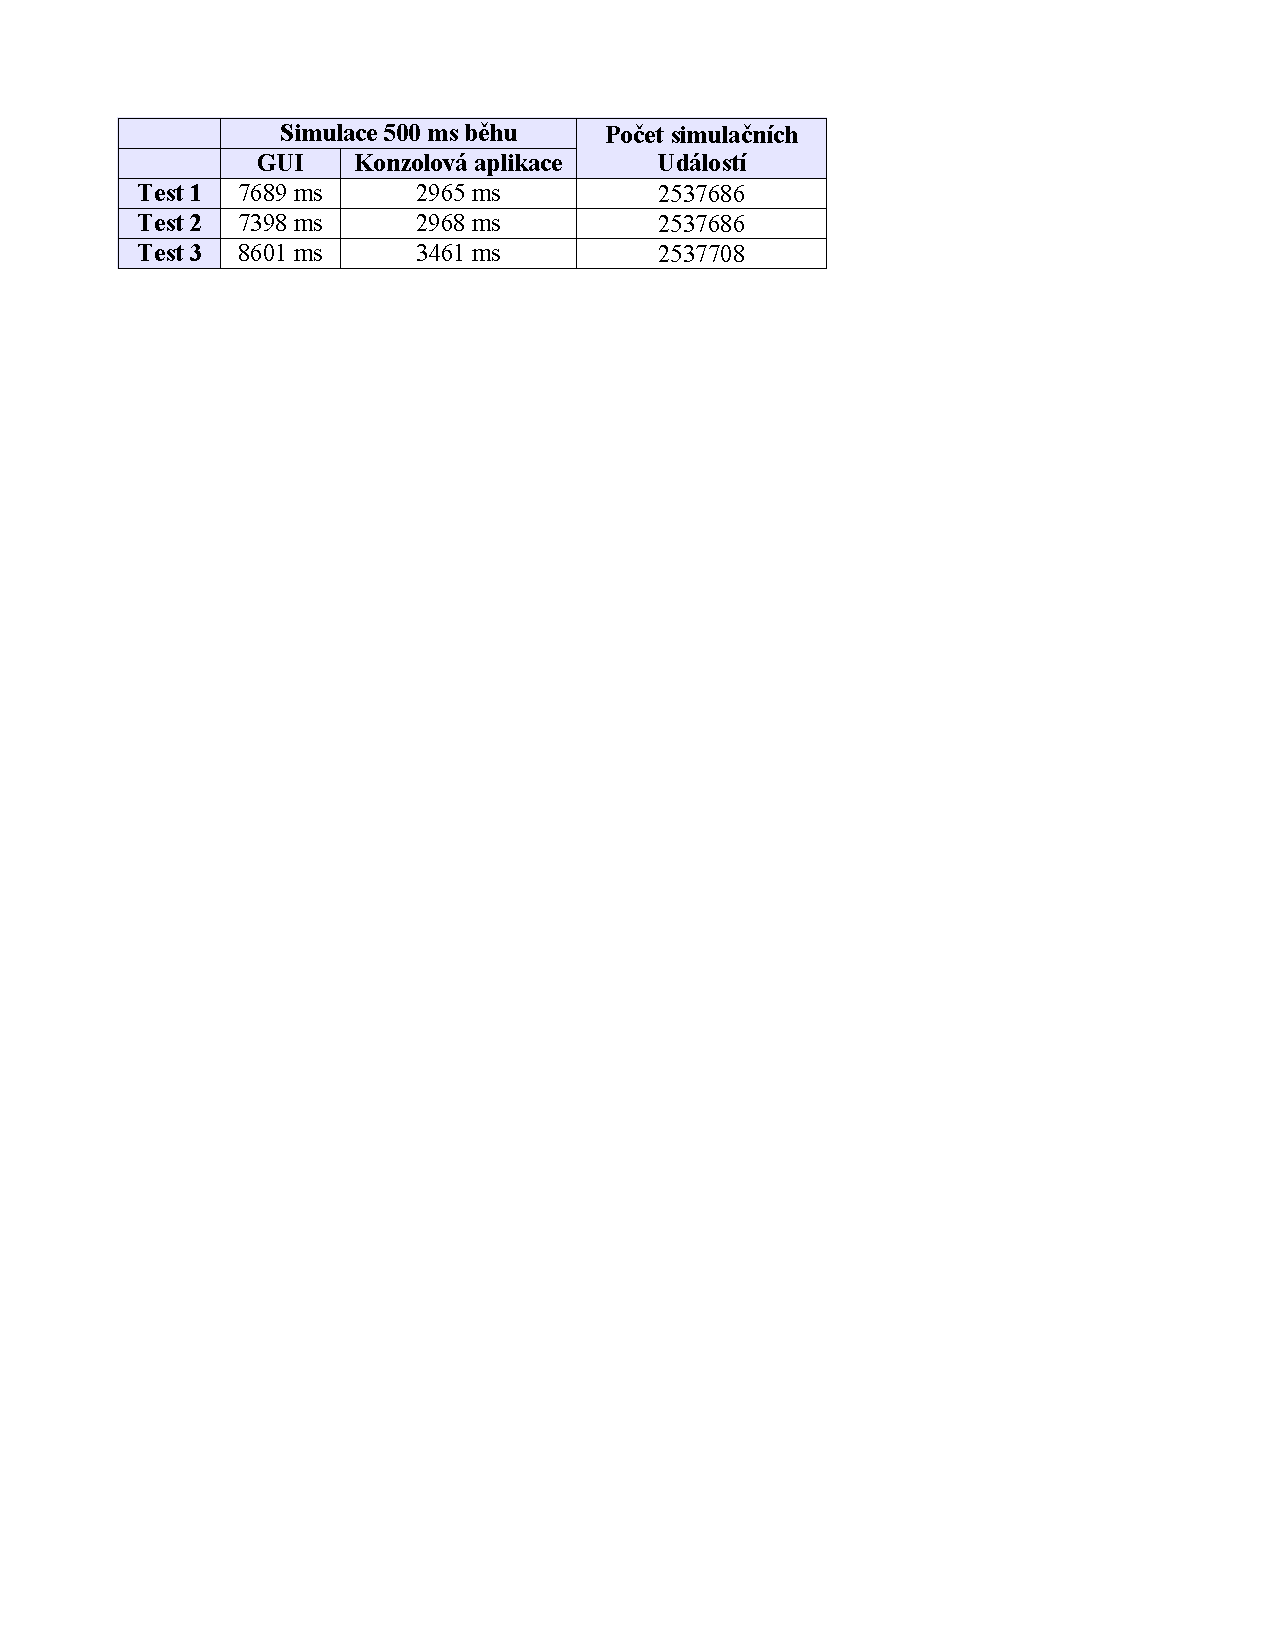
\includegraphics[trim=0cm 23.5cm 2cm 2cm]{fig/tabulka2}
\caption{Tabulka shrnující testy rychlosti simulace na mikrokontroleru řady MSP430x241x o frekvenci 1 262 917 Hz}
\label{fig:tabulka2}
\end{figure}

Stejný výsledek lze očekávat i při použití jiných periferií (například i externích modulů). Čím více simulačních událostí bude generováno v malém časovém intervalu, tím pomalejší simulace bude. To je rovněž umocněno tím, že simulace je sekvenční, zatímco na reálném mikrokontroleru běží většina procesů parelelně.

Obrázek \ref{fig:tabulka2} pak zobrazuje výsledky ze simulace na mikrokontroleru řady MSP430x241x o frekvenci 1 262 917 Hz.

Z porovnání obou tabulek je zřejmé, že s nižší frekvencí mikrokontroleru je simulace rychlejší, ale zpracuje se méně instrukcí. To je logické, protože nižší frekvence vede k větší časové prodlevě mezi jednotlivými simulačními událostmi a během 500 ms se jich tím pádem zpracuje méně.

Další tabulka na obrázku \ref{fig:tabulka3} zobrazuje rozdíl v rychlosti simulace stejné externí komponenty (v tomto případě oscilátoru) implementovaného v jazyce C++ a Python. Jedná se o dobu trvání 500 ms simulace, kdy všechny simulační události byly generovány právě tímto jediným oscilátorem tikajícím o frekvenci 7 372 800 Hz.

\begin{figure}[ht]
\centering
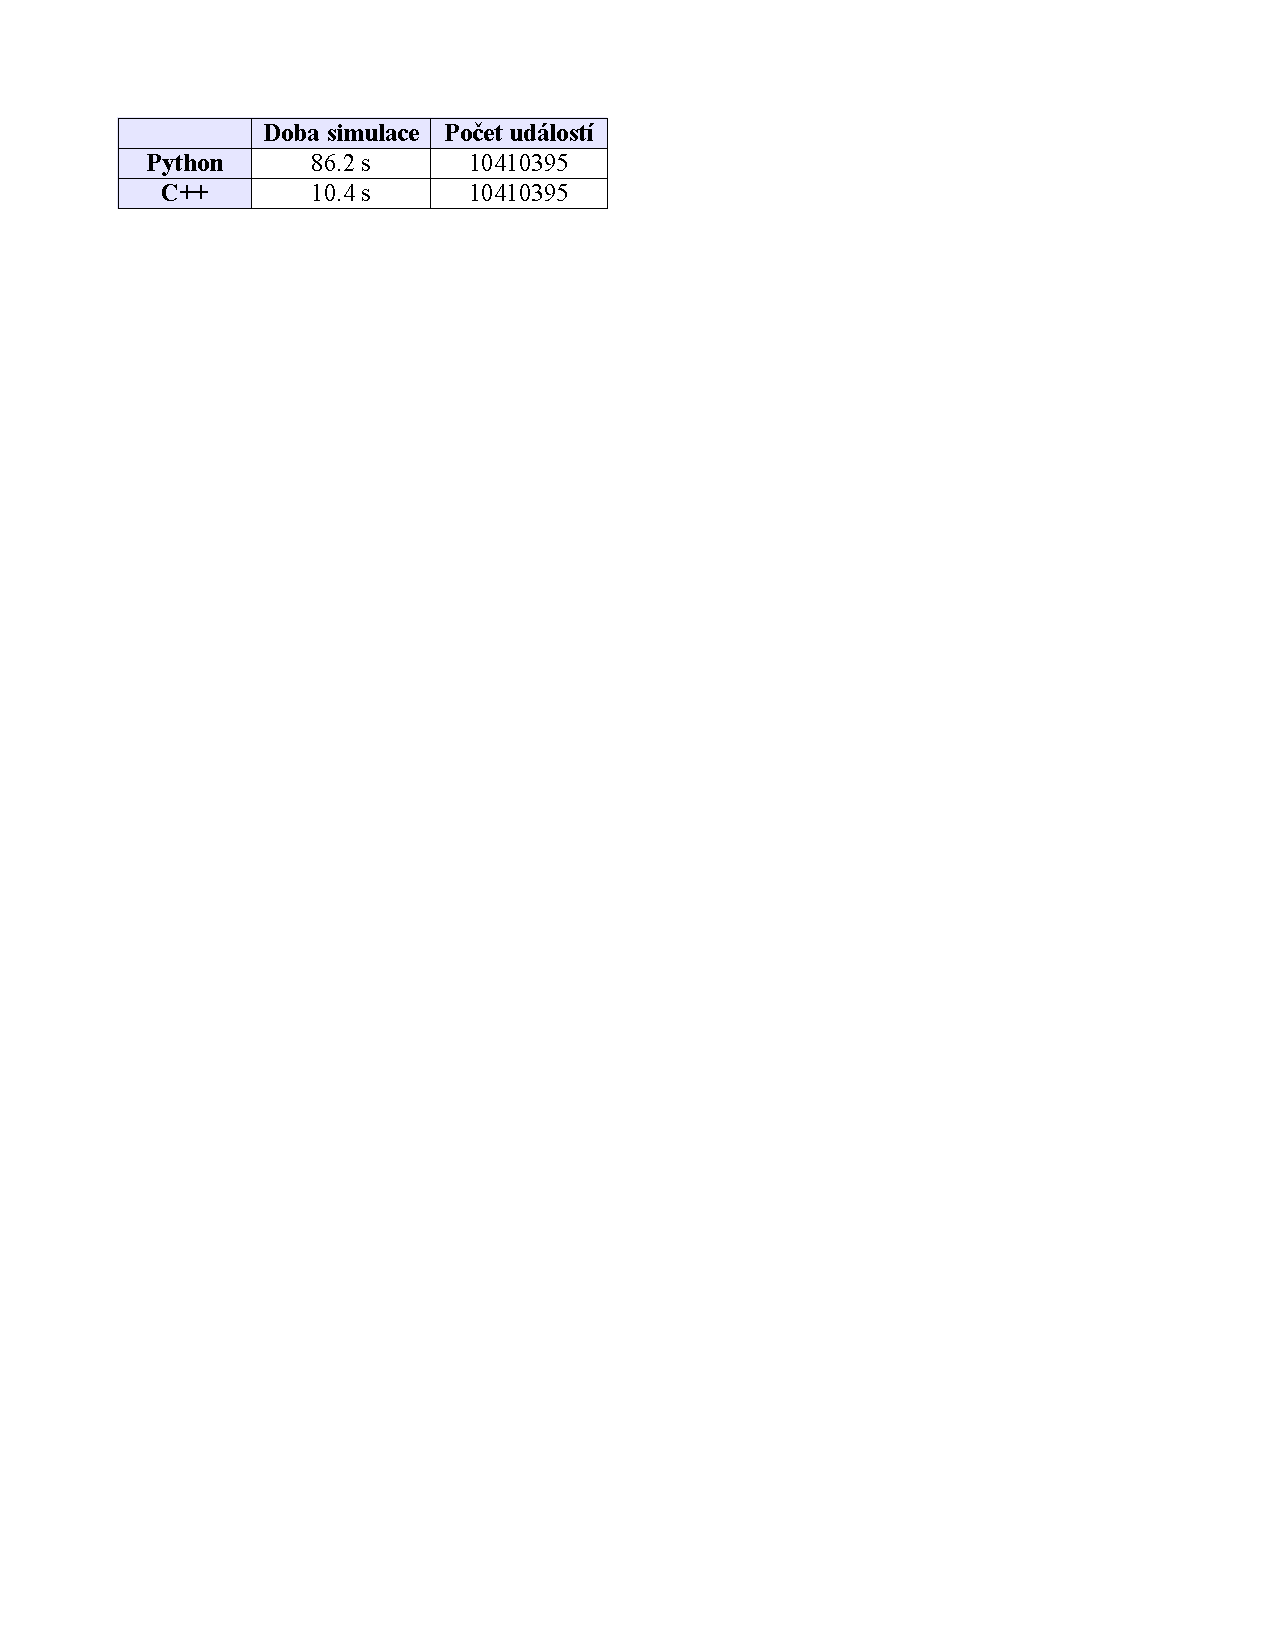
\includegraphics[trim=-2cm 24.5cm 5cm 2cm]{fig/tabulka3}
\caption{Tabulka zobrazující rozdíl mezi implementací oscilátoru v jazyce Python a jazyce C++.}
\label{fig:tabulka3}
\end{figure}

Z tabulky vyplývá, že simulování této konkrétní komponenty v jazyce Python je až 8x pomalejší než simulace stejného chování implementovaného v jazyce C++. Z principu bude vždy simulace komponent v jazyce Python pomalejší, protože dochází ke změně kontextu z C++ do interpretu Python a rovněž dochází ke změně struktur, ve kterých jsou uloženy simulační události.

Při simulaci komponent, které negenerují simulační události ve velké míře (například tlačítko, LED dioda nebo například LCD displej), je rychlost simulace dostačující. Pokud však simulovaná komponenta generuje velké množství událostí (například oscilátor), je vhodné ji implementovat kvůli rychlosti v jazyce C++.

\chapter{Tvorba modulů rozšiřujících základní funkci}
\label{pripad}

Cílem této kapitoly je popsat a názorně ukázat modulárnost implementovaného simulátoru prostřednictvím tvorby dvou nových periferií - tlačítka a oscilátoru. Pro názornost bude tlačítko naprogramováno v jazyce Python a oscilátor v jazyce C++. Tato kapitola rovněž prakticky popisuje rozhraní pro tvorbu nových modulů pro oba tyto jazyky.

\section{Rozšíření simulátoru o tlačítko v jazyce Python}
\label{tlacitko}

Tlačítko je jednoduchou periferií měnící svůj výstup na základě svého vnitřního stavu. Uživateli je umožněno tlačítko stisknout, čímž dojde ke změně jeho stavu a tím pádem i výstupu. Výstup tlačítka v závislosti na jeho stavu (tzv. je-li výstup při sepnutém tlačítku logiká 1 nebo 0) bude konfigurovatelný.

První část rozšíření simulátoru o novou periferii spočívá ve tvorbě XML souboru popisující nově vytvářenou periferii. Simulátor informace z tohoto XML souboru zobrazuje ve svém grafickém uživalském rozhraní a využívá jich rovněž k nalezení samotného skriptu v jazyce Python definujícího chování periferie.

Tento XML soubor musí být pojmenován "peripheral.xml" a musí obsahovat všechny údaje z následujícího příkladu:

\lstset{language=XML, numbers=left, frame=single, breaklines=true, tabsize=2, xleftmargin=20pt}
\begin{lstlisting}
<peripheral type='python'>
   <name>Button</name>
   <comment>Button</comment>
   <author>Jan Kaluza</author>
   <email>hanzz.k@gmail.com</email>
   <version>0.1</version>
   <license>GNU/GPL</license>
   <library>button</library>
</peripheral>
\end{lstlisting}

Jednotlivé řádky definují metadata o dané rozšiřující periferii. Důležitý je zejména element "library", jehož hodnota určuje název skriptu v jazyce Python (bez přípony ".py"), který se simulátor pokusí načíst.

\subsection{Tvorba modulu v jazyce Python}

V této podkapitole je postupně popsán celý modul implementující tlačítko. Každý rozšiřující modul musí obsahovat třídu Peripheral a importovat knihovny PythonQt:

\lstset{language=Python, numbers=left, frame=single, breaklines=true, tabsize=2, xleftmargin=20pt, literate=%
    {á}{{\'a}}1
    {č}{{\v{c}}}1
    {ď}{{\v{d}}}1
    {é}{{\'e}}1
    {ě}{{\v{e}}}1
    {í}{{\'i}}1
    {ň}{{\v{n}}}1
    {ó}{{\'o}}1
    {ř}{{\v{r}}}1
    {š}{{\v{s}}}1
    {ť}{{\v{t}}}1
    {ú}{{\'u}}1
    {ů}{{\r{u}}}1
    {ý}{{\'y}}1
    {ž}{{\v{z}}}1
    {Á}{{\'A}}1
    {Č}{{\v{C}}}1
    {Ď}{{\v{D}}}1
    {É}{{\'E}}1
    {Ě}{{\v{E}}}1
    {Í}{{\'I}}1
    {Ň}{{\v{N}}}1
    {Ó}{{\'O}}1
    {Ř}{{\v{R}}}1
    {Š}{{\v{S}}}1
    {Ť}{{\v{T}}}1
    {Ú}{{\'U}}1
    {Ů}{{\r{U}}}1
    {Ý}{{\'Y}}1
    {Ž}{{\v{Z}}}1}
\begin{lstlisting}
from PythonQt.QtCore import *
from PythonQt.QtGui import *

class Peripheral():
\end{lstlisting}

Při vytvoření nové instance tlačítka v simulátoru je vytvořena nová instance třídy Peripheral a spuštěn její konstruktor:

\lstset{language=Python, numbers=left, frame=single, breaklines=true, tabsize=2, xleftmargin=20pt, firstnumber=5, literate=%
    {á}{{\'a}}1
    {č}{{\v{c}}}1
    {ď}{{\v{d}}}1
    {é}{{\'e}}1
    {ě}{{\v{e}}}1
    {í}{{\'i}}1
    {ň}{{\v{n}}}1
    {ó}{{\'o}}1
    {ř}{{\v{r}}}1
    {š}{{\v{s}}}1
    {ť}{{\v{t}}}1
    {ú}{{\'u}}1
    {ů}{{\r{u}}}1
    {ý}{{\'y}}1
    {ž}{{\v{z}}}1
    {Á}{{\'A}}1
    {Č}{{\v{C}}}1
    {Ď}{{\v{D}}}1
    {É}{{\'E}}1
    {Ě}{{\v{E}}}1
    {Í}{{\'I}}1
    {Ň}{{\v{N}}}1
    {Ó}{{\'O}}1
    {Ř}{{\v{R}}}1
    {Š}{{\v{S}}}1
    {Ť}{{\v{T}}}1
    {Ú}{{\'U}}1
    {Ů}{{\r{U}}}1
    {Ý}{{\'Y}}1
    {Ž}{{\v{Z}}}1}
\begin{lstlisting}
	def __init__(self):
		# Povinné proměnné potřebné pro simulátor:
		self.width = 36		# Šířka tlačítka v pixelech
		self.height = 36	# Výška tlačítka v pixelech
		self.pins = []		# Seznam pinů
		self.pins.append(QRect(24, 12, 12, 12))	# Souřadnice pinu
		self.options = []	# Seznam voleb v kontextovém menu
		# + určuje zaškrtnutou zaškrtávací volbu
		self.options.append("+High when pushed")

		# Proměnné použité pouze tímto modulem:
		self.state = False	# Stav tlačítka
		self.highWhenPushed = True	# Tlačítko generuje 1 při stisknutí
		self.out = []	# události připravené ke generování
\end{lstlisting}

V konstruktoru jsou nejprve inicializovány proměnné potřebné pro správnou funkci simulátoru. Jedná se o rozměry periferie, seznam pinů a seznam voleb zobrazených v kontextovém menu tlačítka. Dále jsou vytvořeny proměnné využité v dalším metodách tlačítka.

\subsubsection{Vykreslení tlačítka}

K vykreslení periferie slouží metoda paint(...):

\lstset{language=Python, numbers=left, frame=single, breaklines=true, tabsize=2, xleftmargin=20pt, firstnumber=19, literate=%
    {á}{{\'a}}1
    {č}{{\v{c}}}1
    {ď}{{\v{d}}}1
    {é}{{\'e}}1
    {ě}{{\v{e}}}1
    {í}{{\'i}}1
    {ň}{{\v{n}}}1
    {ó}{{\'o}}1
    {ř}{{\v{r}}}1
    {š}{{\v{s}}}1
    {ť}{{\v{t}}}1
    {ú}{{\'u}}1
    {ů}{{\r{u}}}1
    {ý}{{\'y}}1
    {ž}{{\v{z}}}1
    {Á}{{\'A}}1
    {Č}{{\v{C}}}1
    {Ď}{{\v{D}}}1
    {É}{{\'E}}1
    {Ě}{{\v{E}}}1
    {Í}{{\'I}}1
    {Ň}{{\v{N}}}1
    {Ó}{{\'O}}1
    {Ř}{{\v{R}}}1
    {Š}{{\v{S}}}1
    {Ť}{{\v{T}}}1
    {Ú}{{\'U}}1
    {Ů}{{\r{U}}}1
    {Ý}{{\'Y}}1
    {Ž}{{\v{Z}}}1}
\begin{lstlisting}
	def paint(self):
		p = QPainter();
		p.begin(self.screen);
		# Vykreslení obrysu tlačítka
		p.drawRect(self.x, self.y + 6, 24, 24)

		color = Qt.black	# Standardní barva výplně
		if self.state:		# Pokud je tlačítko sepnuto ...
			color = Qt.green	# ... zvolíme zelenou barvu

		# Vykreslení symbolu tlačítka
		p.setPen(QPen(Qt.black, 2, Qt.SolidLine))
		p.setBrush(QBrush(color))
		p.drawLine(self.x + 3, self.y + 18, self.x + 3, self.y + 18);
		p.drawLine(self.x + 22, self.y + 18, self.x + 22, self.y + 18);
		if self.state:
			p.drawLine(self.x + 8, self.y + 18, self.x + 18, self.y + 18);
		else:
			p.drawLine(self.x + 8, self.y + 18, self.x + 18, self.y + 12);

		p.setPen(QPen(Qt.black, 1, Qt.SolidLine))
		p.setBrush(QBrush())
		p.drawEllipse(self.x + 3, self.y + 16, 4, 4);
		p.drawEllipse(self.x + 17, self.y + 16, 4, 4);

		# Vykreslení pinu na pouzdře tlačítka
		for rect in self.pins:
			if self.state == self.highWhenPushed:
				p.fillRect(rect, QBrush(QColor(0,255,0)))
			p.drawRect(rect)
\end{lstlisting}

Tato metoda využíva vykreslování pomocí knihovny Qt, konkrétně její třídy QPainter. Vykreslování probíha na objekt self.screen reprezentující kreslící plochu GUI. Programátor tak má velkou svobodu v ovlivnění vzhledu periferie.

\subsubsection{Implementace logiky tlačítka}

Pro správnou funkci tlačítka je potřeba, aby došlo při stisknutí tlačítka k vygenerování odpovídajícího signálu na jeho pinu. O kliknutí je tlačítko informováno zavoláním jeho metody clicked(...):

\lstset{language=Python, numbers=left, frame=single, breaklines=true, tabsize=2, xleftmargin=20pt, firstnumber=49, literate=%
    {á}{{\'a}}1
    {č}{{\v{c}}}1
    {ď}{{\v{d}}}1
    {é}{{\'e}}1
    {ě}{{\v{e}}}1
    {í}{{\'i}}1
    {ň}{{\v{n}}}1
    {ó}{{\'o}}1
    {ř}{{\v{r}}}1
    {š}{{\v{s}}}1
    {ť}{{\v{t}}}1
    {ú}{{\'u}}1
    {ů}{{\r{u}}}1
    {ý}{{\'y}}1
    {ž}{{\v{z}}}1
    {Á}{{\'A}}1
    {Č}{{\v{C}}}1
    {Ď}{{\v{D}}}1
    {É}{{\'E}}1
    {Ě}{{\v{E}}}1
    {Í}{{\'I}}1
    {Ň}{{\v{N}}}1
    {Ó}{{\'O}}1
    {Ř}{{\v{R}}}1
    {Š}{{\v{S}}}1
    {Ť}{{\v{T}}}1
    {Ú}{{\'U}}1
    {Ů}{{\r{U}}}1
    {Ý}{{\'Y}}1
    {Ž}{{\v{Z}}}1}
\begin{lstlisting}
	def clicked(self, p):	# p: (x,y) pozice myši
		self.state = not self.state	# Přepnutí tlačítka
		self.screen.update()	# Požadavek o překreslení
		# Vygenerování (X,Y) výstupu podle aktuálního nastavení
		# X: index pinu pro který se generuje výstup
		# Y: hodnota napětí na výstupním pinu
		if self.state:
			if self.highWhenPushed:
				self.out.append((0, 3.0))
			else:
				self.out.append((0, 0.0))
		else:
			if self.highWhenPushed:
				self.out.append((0, 0.0))
			else:
				self.out.append((0, 3.0))
		# Informování simulátoru, že je k dispozici nový výstup
		self.hasNewOutput = True
\end{lstlisting}

V případě, že uživatel na tlačítko klikne, je změněn jeho stav a vygenerován nový výstup do výstupního seznamu "self.out". Simulátor po zavolání metody clicked(...) ověří hodnotu proměnné "self.hasNewOutput". Prokud je tato proměnná nastavena na True, je zavolána metoda timeAdvance(...) pro naplánování času , kdy se má výstupní událost uskutečnit.

\lstset{language=Python, numbers=left, frame=single, breaklines=true, tabsize=2, xleftmargin=20pt, firstnumber=67, literate=%
    {á}{{\'a}}1
    {č}{{\v{c}}}1
    {ď}{{\v{d}}}1
    {é}{{\'e}}1
    {ě}{{\v{e}}}1
    {í}{{\'i}}1
    {ň}{{\v{n}}}1
    {ó}{{\'o}}1
    {ř}{{\v{r}}}1
    {š}{{\v{s}}}1
    {ť}{{\v{t}}}1
    {ú}{{\'u}}1
    {ů}{{\r{u}}}1
    {ý}{{\'y}}1
    {ž}{{\v{z}}}1
    {Á}{{\'A}}1
    {Č}{{\v{C}}}1
    {Ď}{{\v{D}}}1
    {É}{{\'E}}1
    {Ě}{{\v{E}}}1
    {Í}{{\'I}}1
    {Ň}{{\v{N}}}1
    {Ó}{{\'O}}1
    {Ř}{{\v{R}}}1
    {Š}{{\v{S}}}1
    {Ť}{{\v{T}}}1
    {Ú}{{\'U}}1
    {Ů}{{\r{U}}}1
    {Ý}{{\'Y}}1
    {Ž}{{\v{Z}}}1}
\begin{lstlisting}
	def timeAdvance(self):
		# Pokud máme výstupní signál, výstup musí být okamžitý
		if not len(self.out) == 0:
			return 0
		# V opačném případě vrátíme dostatečně velké číslo
		return 365
\end{lstlisting}

Metoda timeAdvance(...) je volána simulátorem v případě, kdy je potřeba naplánovat další akci periferie. Po startu simulace je tato metoda zavolána pro naplánování první akce tlačítka. Jelikož tlačítko není autonomní a neprovádí samo od sebe žádné akce, tak v případě, kdy není k naplánován žádný výstupní signál, naplánuje svou další akci do velmi vzdálené budoucnosti. Tím je zajištěno, že simulátor nebude volat žádné metody tlačítka aniž by to tlačítko samo nevyžádalo pomocí proměnné "self.hasNewOutput".

V případě, kdy má tlačítko naplánován výstup, vrací číslo 0, čímž říká simulátoru, že chce svou další akci spustit okamžitě. Simulátor na tento požadavek reaguje zavoláním metody internalEvent(...). Protože však tlačítko neprovádí žádné autonomní naplánované změny stavu, je tato metoda prázdná:

\lstset{language=Python, numbers=left, frame=single, breaklines=true, tabsize=2, xleftmargin=20pt, firstnumber=73, literate=%
    {á}{{\'a}}1
    {č}{{\v{c}}}1
    {ď}{{\v{d}}}1
    {é}{{\'e}}1
    {ě}{{\v{e}}}1
    {í}{{\'i}}1
    {ň}{{\v{n}}}1
    {ó}{{\'o}}1
    {ř}{{\v{r}}}1
    {š}{{\v{s}}}1
    {ť}{{\v{t}}}1
    {ú}{{\'u}}1
    {ů}{{\r{u}}}1
    {ý}{{\'y}}1
    {ž}{{\v{z}}}1
    {Á}{{\'A}}1
    {Č}{{\v{C}}}1
    {Ď}{{\v{D}}}1
    {É}{{\'E}}1
    {Ě}{{\v{E}}}1
    {Í}{{\'I}}1
    {Ň}{{\v{N}}}1
    {Ó}{{\'O}}1
    {Ř}{{\v{R}}}1
    {Š}{{\v{S}}}1
    {Ť}{{\v{T}}}1
    {Ú}{{\'U}}1
    {Ů}{{\r{U}}}1
    {Ý}{{\'Y}}1
    {Ž}{{\v{Z}}}1}
\begin{lstlisting}
	def InternalEvent(self):
		pass
\end{lstlisting}

Dalším krokem simulátoru je zavolání metody output(...):

\lstset{language=Python, numbers=left, frame=single, breaklines=true, tabsize=2, xleftmargin=20pt, firstnumber=75, literate=%
    {á}{{\'a}}1
    {č}{{\v{c}}}1
    {ď}{{\v{d}}}1
    {é}{{\'e}}1
    {ě}{{\v{e}}}1
    {í}{{\'i}}1
    {ň}{{\v{n}}}1
    {ó}{{\'o}}1
    {ř}{{\v{r}}}1
    {š}{{\v{s}}}1
    {ť}{{\v{t}}}1
    {ú}{{\'u}}1
    {ů}{{\r{u}}}1
    {ý}{{\'y}}1
    {ž}{{\v{z}}}1
    {Á}{{\'A}}1
    {Č}{{\v{C}}}1
    {Ď}{{\v{D}}}1
    {É}{{\'E}}1
    {Ě}{{\v{E}}}1
    {Í}{{\'I}}1
    {Ň}{{\v{N}}}1
    {Ó}{{\'O}}1
    {Ř}{{\v{R}}}1
    {Š}{{\v{S}}}1
    {Ť}{{\v{T}}}1
    {Ú}{{\'U}}1
    {Ů}{{\r{U}}}1
    {Ý}{{\'Y}}1
    {Ž}{{\v{Z}}}1}
\begin{lstlisting}
	def output(self):
		if len(self.out) == 0:
			return ()
		return self.out.pop(0)
\end{lstlisting}

Pokud je k naplánována výstupní událost v proměnné "self.out", je tato událost předána simulátoru. Ten ji pak přepošle v závislosti na zapojení cílové periferii a zavolá znovu metodu output(...). Pokud již nejsou k dispozici žádné události, je vrácena prázdná událost a opět zavolána metoda timeAdvance(...) pro naplánování další události tlačítka.

Pokud by tlačítko přijímalo na svém pinu vstupní události, byly by tlačítku doručeny pomocí metody externalEvent(...). Jelikož však tlačítko události pouze generuje, je tato metoda prázdná:

\lstset{language=Python, numbers=left, frame=single, breaklines=true, tabsize=2, xleftmargin=20pt, firstnumber=79, literate=%
    {á}{{\'a}}1
    {č}{{\v{c}}}1
    {ď}{{\v{d}}}1
    {é}{{\'e}}1
    {ě}{{\v{e}}}1
    {í}{{\'i}}1
    {ň}{{\v{n}}}1
    {ó}{{\'o}}1
    {ř}{{\v{r}}}1
    {š}{{\v{s}}}1
    {ť}{{\v{t}}}1
    {ú}{{\'u}}1
    {ů}{{\r{u}}}1
    {ý}{{\'y}}1
    {ž}{{\v{z}}}1
    {Á}{{\'A}}1
    {Č}{{\v{C}}}1
    {Ď}{{\v{D}}}1
    {É}{{\'E}}1
    {Ě}{{\v{E}}}1
    {Í}{{\'I}}1
    {Ň}{{\v{N}}}1
    {Ó}{{\'O}}1
    {Ř}{{\v{R}}}1
    {Š}{{\v{S}}}1
    {Ť}{{\v{T}}}1
    {Ú}{{\'U}}1
    {Ů}{{\r{U}}}1
    {Ý}{{\'Y}}1
    {Ž}{{\v{Z}}}1}
\begin{lstlisting}
	def externalEvent(self, pin, value):
		pass
\end{lstlisting}

\subsubsection{Konfigurování tlačítka}

Tlačítko disponuje jedinou konfigurační volbou - lze u něj nastavit, bude-li po sepnutí ve stavu logické 1 nebo 0. Toto nastavení je potřeba ukládat a načítat společne s projektem. K tomuto účelu slouží metody save(...) a load(...). Pro jednodušší přidávání nových voleb je implementována rovněž metoda simpleParser(...) umožňující jednoduché parsování XML dat. Místo této metody by však bylo možno využít plnohodnotného Pythonního modulu parsujícího XML formát.
\lstset{language=Python, numbers=left, frame=single, breaklines=true, tabsize=2, xleftmargin=20pt, firstnumber=81, literate=%
    {á}{{\'a}}1
    {č}{{\v{c}}}1
    {ď}{{\v{d}}}1
    {é}{{\'e}}1
    {ě}{{\v{e}}}1
    {í}{{\'i}}1
    {ň}{{\v{n}}}1
    {ó}{{\'o}}1
    {ř}{{\v{r}}}1
    {š}{{\v{s}}}1
    {ť}{{\v{t}}}1
    {ú}{{\'u}}1
    {ů}{{\r{u}}}1
    {ý}{{\'y}}1
    {ž}{{\v{z}}}1
    {Á}{{\'A}}1
    {Č}{{\v{C}}}1
    {Ď}{{\v{D}}}1
    {É}{{\'E}}1
    {Ě}{{\v{E}}}1
    {Í}{{\'I}}1
    {Ň}{{\v{N}}}1
    {Ó}{{\'O}}1
    {Ř}{{\v{R}}}1
    {Š}{{\v{S}}}1
    {Ť}{{\v{T}}}1
    {Ú}{{\'U}}1
    {Ů}{{\r{U}}}1
    {Ý}{{\'Y}}1
    {Ž}{{\v{Z}}}1}
\begin{lstlisting}
	def save(self):
		# Uložení dat do XML souboru
		return "<highWhenPushed>" + str(self.highWhenPushed) + "</highWhenPushed>"

	def simpleParser(self, xml, tag):
		# Získání hodnoty elementu "tag" z XML dat
		start = xml.find("<" + tag + ">")
		end = xml.find("</" + tag + ">")
		if start == -1 or end == -1:
			return None
		return xml[start + len(tag) + 2 : end]

	def load(self, xml):
		# Načtení hodnoty elementu "highWhenPushed"
		c = self.simpleParser(xml, "highWhenPushed")
		if c != None and c == "False":
			self.highWhenPushed = False
\end{lstlisting}

\section{Rozšíření simulátoru o oscilátor v jazyce C++}
\label{oscilator}

Oscilátor je periferie, která svůj výstup mění pravidelně v určité frekvenci. Pokud periferie pracuje po celou dobu simulace, je vhodné ji kvůli vyššímu výkonu naprogramovat v jazyce C++.

Podobně jako u periferie v jazyce Python je nutné i u oscilátoru definovat XML soubor "peripheral.xml" popisující nově vytvářenou periferii:

\lstset{language=XML, numbers=left, frame=single, breaklines=true, tabsize=2, xleftmargin=20pt}
\begin{lstlisting}
<peripheral type='binary'>
   <name>Crystal oscillator</name>
   <comment>Crystal oscillator</comment>
   <author>Jan Kaluza</author>
   <email>hanzz.k@gmail.com</email>
   <version>0.1</version>
   <license>GNU/GPL</license>
   <library>oscillator</library>
</peripheral>
\end{lstlisting}

Na rozdíl od periferie v jazyce Python je zde použit typ "binary" udávájící, že se jedná o binární modul reprezentovaný sdílenou knihovnou.

\subsection{Tvorba modulu v jazyce C++}

V jazyku C++ je kód modulu tvořen dvěma soubory - hlavičkovým souborem popisujícím rozhraní hlavní třídy modulu a souborem se samotnou její implementací.

\subsubsection{Deklarace třídy modulu}

Třída modulu deklaruje rozhraní modulu. Jednotlivé funkce budou podrobněji popsány v části zabývající se jejich implementací.

\lstset{language=Python, numbers=left, frame=single, breaklines=true, tabsize=2, xleftmargin=20pt, firstnumber=1, literate=%
    {á}{{\'a}}1
    {č}{{\v{c}}}1
    {ď}{{\v{d}}}1
    {é}{{\'e}}1
    {ě}{{\v{e}}}1
    {í}{{\'i}}1
    {ň}{{\v{n}}}1
    {ó}{{\'o}}1
    {ř}{{\v{r}}}1
    {š}{{\v{s}}}1
    {ť}{{\v{t}}}1
    {ú}{{\'u}}1
    {ů}{{\r{u}}}1
    {ý}{{\'y}}1
    {ž}{{\v{z}}}1
    {Á}{{\'A}}1
    {Č}{{\v{C}}}1
    {Ď}{{\v{D}}}1
    {É}{{\'E}}1
    {Ě}{{\v{E}}}1
    {Í}{{\'I}}1
    {Ň}{{\v{N}}}1
    {Ó}{{\'O}}1
    {Ř}{{\v{R}}}1
    {Š}{{\v{S}}}1
    {Ť}{{\v{T}}}1
    {Ú}{{\'U}}1
    {Ů}{{\r{U}}}1
    {Ý}{{\'Y}}1
    {Ž}{{\v{Z}}}1}
\begin{lstlisting}
class Oscillator : public Peripheral {
	public:
		Oscillator();

		// Metoda volána při interní změně
		void internalTransition();

		// Metoda volána při externí události
		void externalEvent(double e, const SimulationEventList &);

		// Metoda volána při generování výstupu
		void output(SimulationEventList &output);

		// Metoda plánující čas dálší akce
		double timeAdvance();

		// Reset oscilátoru
		void reset();

		// Vykreslení oscilátoru
		void paint(QWidget *screen);

		// Definice pinů oscilátoru
		PinList &getPins() { return m_pins; }

		// Definice konfiguračních voleb
		const QStringList &getOptions();

		// Spuštění konfiguráční volby
		void executeOption(int option);

		// Uložení a nahrání konfiguračních voleb
		void save(QTextStream &stream);
		void load(QDomElement &object, QString &error);

	private:
		PinList m_pins;
		bool m_state;
		unsigned long m_freq;
		double m_step;
		SimulationEventList m_output;
		QStringList m_options;

};
\end{lstlisting}

\subsubsection{Deklarace třídy vytvářející instance modulu}

Aby bylo možné vytvořit více instancí modulu v rámci jednoho projektu, je potřeba definovat také třídu dědící z třídy PeripheralInterface. Účelem této třídy je vytvoření nové instance modulu metodou create().

\lstset{language=Python, numbers=left, frame=single, breaklines=true, tabsize=2, xleftmargin=20pt, firstnumber=45, literate=%
    {á}{{\'a}}1
    {č}{{\v{c}}}1
    {ď}{{\v{d}}}1
    {é}{{\'e}}1
    {ě}{{\v{e}}}1
    {í}{{\'i}}1
    {ň}{{\v{n}}}1
    {ó}{{\'o}}1
    {ř}{{\v{r}}}1
    {š}{{\v{s}}}1
    {ť}{{\v{t}}}1
    {ú}{{\'u}}1
    {ů}{{\r{u}}}1
    {ý}{{\'y}}1
    {ž}{{\v{z}}}1
    {Á}{{\'A}}1
    {Č}{{\v{C}}}1
    {Ď}{{\v{D}}}1
    {É}{{\'E}}1
    {Ě}{{\v{E}}}1
    {Í}{{\'I}}1
    {Ň}{{\v{N}}}1
    {Ó}{{\'O}}1
    {Ř}{{\v{R}}}1
    {Š}{{\v{S}}}1
    {Ť}{{\v{T}}}1
    {Ú}{{\'U}}1
    {Ů}{{\r{U}}}1
    {Ý}{{\'Y}}1
    {Ž}{{\v{Z}}}1}
\begin{lstlisting}
class OscillatorInterface : public QObject, PeripheralInterface {
	Q_OBJECT
	Q_INTERFACES(PeripheralInterface)

	public:
		Peripheral *create();
};
\end{lstlisting}

\subsubsection{Konstruktor třídy Oscillator}

V rámci konstruktoru třídy Oscillator je potřeba nastavit jeho velikost pro vykreslování, definovat jeho piny, prvotní frekvenci a seznam konfiguračních voleb:

\lstset{language=Python, numbers=left, frame=single, breaklines=true, tabsize=2, xleftmargin=20pt, firstnumber=10, literate=%
    {á}{{\'a}}1
    {č}{{\v{c}}}1
    {ď}{{\v{d}}}1
    {é}{{\'e}}1
    {ě}{{\v{e}}}1
    {í}{{\'i}}1
    {ň}{{\v{n}}}1
    {ó}{{\'o}}1
    {ř}{{\v{r}}}1
    {š}{{\v{s}}}1
    {ť}{{\v{t}}}1
    {ú}{{\'u}}1
    {ů}{{\r{u}}}1
    {ý}{{\'y}}1
    {ž}{{\v{z}}}1
    {Á}{{\'A}}1
    {Č}{{\v{C}}}1
    {Ď}{{\v{D}}}1
    {É}{{\'E}}1
    {Ě}{{\v{E}}}1
    {Í}{{\'I}}1
    {Ň}{{\v{N}}}1
    {Ó}{{\'O}}1
    {Ř}{{\v{R}}}1
    {Š}{{\v{S}}}1
    {Ť}{{\v{T}}}1
    {Ú}{{\'U}}1
    {Ů}{{\r{U}}}1
    {Ý}{{\'Y}}1
    {Ž}{{\v{Z}}}1}
\begin{lstlisting}
Oscillator::Oscillator() : m_state(false) {
	resize(36, 24);

	m_pins.push_back(Pin(QRect(24, 0, 10, 10), "XIN", 0));
	m_pins.push_back(Pin(QRect(24, 12, 10, 10), "XOUT", 0));

	m_freq = 7372800;
	m_step = 1.0 / m_freq / 2;

	m_options << "Set frequency";
}
\end{lstlisting}

\subsubsection{Vykreslení oscilátoru }

Vykreslení oscilátoru probíha v metodě paint(...). Tato metody vykreslí značku oscilátoru a oba jeho piny. Pokud je pin aktivní, má zelenou barvu.

\lstset{language=Python, numbers=left, frame=single, breaklines=true, tabsize=2, xleftmargin=20pt, firstnumber=21, literate=%
    {á}{{\'a}}1
    {č}{{\v{c}}}1
    {ď}{{\v{d}}}1
    {é}{{\'e}}1
    {ě}{{\v{e}}}1
    {í}{{\'i}}1
    {ň}{{\v{n}}}1
    {ó}{{\'o}}1
    {ř}{{\v{r}}}1
    {š}{{\v{s}}}1
    {ť}{{\v{t}}}1
    {ú}{{\'u}}1
    {ů}{{\r{u}}}1
    {ý}{{\'y}}1
    {ž}{{\v{z}}}1
    {Á}{{\'A}}1
    {Č}{{\v{C}}}1
    {Ď}{{\v{D}}}1
    {É}{{\'E}}1
    {Ě}{{\v{E}}}1
    {Í}{{\'I}}1
    {Ň}{{\v{N}}}1
    {Ó}{{\'O}}1
    {Ř}{{\v{R}}}1
    {Š}{{\v{S}}}1
    {Ť}{{\v{T}}}1
    {Ú}{{\'U}}1
    {Ů}{{\r{U}}}1
    {Ý}{{\'Y}}1
    {Ž}{{\v{Z}}}1}
\begin{lstlisting}
void Oscillator::paint(QWidget *screen) {
	QPainter qp(screen);
	qp.drawRect(m_x, m_y, m_width - 12, m_height);
	qp.drawLine(m_x + 3 + 9, m_y + 7, m_x + 3 + 9, m_y + 2);
	qp.drawLine(m_x + 3, m_y + 7, m_x + 3 + 18, m_y + 7);
	qp.drawRect(m_x + 3, m_y + 9, 18, 6);
	qp.drawLine(m_x + 3, m_y + 17, m_x + 3 + 18, m_y + 17);
	qp.drawLine(m_x + 3 + 9, m_y + 17, m_x + 3 + 9, m_y + 22);

	for (PinList::iterator it = m_pins.begin(); it != m_pins.end(); it++) {
		if (m_state) {
			qp.fillRect(it->rect, QBrush(QColor(0,255,0)));
		}
		qp.drawRect(it->rect);
	}
}
\end{lstlisting}

\subsubsection{Implementace logiky oscilátoru}

Oscilátor mění svůj výstup pravidelně v závislosti na nastavené frekvenci. Frekvence je uložena v proměnné "m\_freq". V proměnné "m\_step" je pak počítána délka jednoho stavu výstupu. Po startu simulace je nejprve zavolána metoda timeAdvance(...), která naplánuje následující akci oscilátoru (změnu jeho výstupu). Čas této akce je dán právě hodnotou proměnné "m\_step".

\lstset{language=Python, numbers=left, frame=single, breaklines=true, tabsize=2, xleftmargin=20pt, firstnumber=37, literate=%
    {á}{{\'a}}1
    {č}{{\v{c}}}1
    {ď}{{\v{d}}}1
    {é}{{\'e}}1
    {ě}{{\v{e}}}1
    {í}{{\'i}}1
    {ň}{{\v{n}}}1
    {ó}{{\'o}}1
    {ř}{{\v{r}}}1
    {š}{{\v{s}}}1
    {ť}{{\v{t}}}1
    {ú}{{\'u}}1
    {ů}{{\r{u}}}1
    {ý}{{\'y}}1
    {ž}{{\v{z}}}1
    {Á}{{\'A}}1
    {Č}{{\v{C}}}1
    {Ď}{{\v{D}}}1
    {É}{{\'E}}1
    {Ě}{{\v{E}}}1
    {Í}{{\'I}}1
    {Ň}{{\v{N}}}1
    {Ó}{{\'O}}1
    {Ř}{{\v{R}}}1
    {Š}{{\v{S}}}1
    {Ť}{{\v{T}}}1
    {Ú}{{\'U}}1
    {Ů}{{\r{U}}}1
    {Ý}{{\'Y}}1
    {Ž}{{\v{Z}}}1}
\begin{lstlisting}
double Oscillator::timeAdvance() {
	return m_step;
}
\end{lstlisting}

Po uplynutí této časové doby je zavolána metoda internalTransition(...). Cílem této metody je změnit logickou hodnotu na pinech ocilátoru a uložit výstupní sekvenci do proměnné "m\_output":

\lstset{language=Python, numbers=left, frame=single, breaklines=true, tabsize=2, xleftmargin=20pt, firstnumber=40, literate=%
    {á}{{\'a}}1
    {č}{{\v{c}}}1
    {ď}{{\v{d}}}1
    {é}{{\'e}}1
    {ě}{{\v{e}}}1
    {í}{{\'i}}1
    {ň}{{\v{n}}}1
    {ó}{{\'o}}1
    {ř}{{\v{r}}}1
    {š}{{\v{s}}}1
    {ť}{{\v{t}}}1
    {ú}{{\'u}}1
    {ů}{{\r{u}}}1
    {ý}{{\'y}}1
    {ž}{{\v{z}}}1
    {Á}{{\'A}}1
    {Č}{{\v{C}}}1
    {Ď}{{\v{D}}}1
    {É}{{\'E}}1
    {Ě}{{\v{E}}}1
    {Í}{{\'I}}1
    {Ň}{{\v{N}}}1
    {Ó}{{\'O}}1
    {Ř}{{\v{R}}}1
    {Š}{{\v{S}}}1
    {Ť}{{\v{T}}}1
    {Ú}{{\'U}}1
    {Ů}{{\r{U}}}1
    {Ý}{{\'Y}}1
    {Ž}{{\v{Z}}}1}
\begin{lstlisting}
void Oscillator::internalTransition() {
	if (!m_state) {
		m_state = true;
		m_output.insert(SimulationEvent(0, 3.0));
		m_output.insert(SimulationEvent(1, 3.0));
	}
	else {
		m_state = false;
		m_output.insert(SimulationEvent(0, 0.0));
		m_output.insert(SimulationEvent(1, 0.0));
	}
}
\end{lstlisting}

V zápětí na to je zavolána metoda output(...), jejímž úkolem je vygenerování výstupu uloženého v proměnné "m\_output":

\lstset{language=Python, numbers=left, frame=single, breaklines=true, tabsize=2, xleftmargin=20pt, firstnumber=52, literate=%
    {á}{{\'a}}1
    {č}{{\v{c}}}1
    {ď}{{\v{d}}}1
    {é}{{\'e}}1
    {ě}{{\v{e}}}1
    {í}{{\'i}}1
    {ň}{{\v{n}}}1
    {ó}{{\'o}}1
    {ř}{{\v{r}}}1
    {š}{{\v{s}}}1
    {ť}{{\v{t}}}1
    {ú}{{\'u}}1
    {ů}{{\r{u}}}1
    {ý}{{\'y}}1
    {ž}{{\v{z}}}1
    {Á}{{\'A}}1
    {Č}{{\v{C}}}1
    {Ď}{{\v{D}}}1
    {É}{{\'E}}1
    {Ě}{{\v{E}}}1
    {Í}{{\'I}}1
    {Ň}{{\v{N}}}1
    {Ó}{{\'O}}1
    {Ř}{{\v{R}}}1
    {Š}{{\v{S}}}1
    {Ť}{{\v{T}}}1
    {Ú}{{\'U}}1
    {Ů}{{\r{U}}}1
    {Ý}{{\'Y}}1
    {Ž}{{\v{Z}}}1}
\begin{lstlisting}
void Oscillator::output(SimulationEventList &output) {
	if (!m_output.empty()) {
		output.swap(m_output);
	}
}
\end{lstlisting}

Tento postup se stále opakuje, čímž implementuje funkci oscilátoru. Jelikož oscilátor nereaguje na externí události, je implementace metody externalEvent(...) prázdná.

\subsubsection{Konfigurace oscilátoru}

Oscilátor umožňuje změnu své frekvence prostřednictvím dialogu. Grafickému uživatelskému rozhraní jsou informace o podporovaných konfiguračních volbách předány metodou getOptions(...) vracející proměnnou "m\_options" inicializovanou v konstruktoru:

\lstset{language=Python, numbers=left, frame=single, breaklines=true, tabsize=2, xleftmargin=20pt, firstnumber=57, literate=%
    {á}{{\'a}}1
    {č}{{\v{c}}}1
    {ď}{{\v{d}}}1
    {é}{{\'e}}1
    {ě}{{\v{e}}}1
    {í}{{\'i}}1
    {ň}{{\v{n}}}1
    {ó}{{\'o}}1
    {ř}{{\v{r}}}1
    {š}{{\v{s}}}1
    {ť}{{\v{t}}}1
    {ú}{{\'u}}1
    {ů}{{\r{u}}}1
    {ý}{{\'y}}1
    {ž}{{\v{z}}}1
    {Á}{{\'A}}1
    {Č}{{\v{C}}}1
    {Ď}{{\v{D}}}1
    {É}{{\'E}}1
    {Ě}{{\v{E}}}1
    {Í}{{\'I}}1
    {Ň}{{\v{N}}}1
    {Ó}{{\'O}}1
    {Ř}{{\v{R}}}1
    {Š}{{\v{S}}}1
    {Ť}{{\v{T}}}1
    {Ú}{{\'U}}1
    {Ů}{{\r{U}}}1
    {Ý}{{\'Y}}1
    {Ž}{{\v{Z}}}1}
\begin{lstlisting}
const QStringList &Oscillator::getOptions() {
	return m_options;
}
\end{lstlisting}

Pokud uživatel tuto volby vybere, je zavolána metoda executeOption(...) s parametrem definujícím index konfigurační volby. Na to reaguje osciloskop vyvoláním dialogu pro změnu frekvence:

\lstset{language=Python, numbers=left, frame=single, breaklines=true, tabsize=2, xleftmargin=20pt, firstnumber=60, literate=%
    {á}{{\'a}}1
    {č}{{\v{c}}}1
    {ď}{{\v{d}}}1
    {é}{{\'e}}1
    {ě}{{\v{e}}}1
    {í}{{\'i}}1
    {ň}{{\v{n}}}1
    {ó}{{\'o}}1
    {ř}{{\v{r}}}1
    {š}{{\v{s}}}1
    {ť}{{\v{t}}}1
    {ú}{{\'u}}1
    {ů}{{\r{u}}}1
    {ý}{{\'y}}1
    {ž}{{\v{z}}}1
    {Á}{{\'A}}1
    {Č}{{\v{C}}}1
    {Ď}{{\v{D}}}1
    {É}{{\'E}}1
    {Ě}{{\v{E}}}1
    {Í}{{\'I}}1
    {Ň}{{\v{N}}}1
    {Ó}{{\'O}}1
    {Ř}{{\v{R}}}1
    {Š}{{\v{S}}}1
    {Ť}{{\v{T}}}1
    {Ú}{{\'U}}1
    {Ů}{{\r{U}}}1
    {Ý}{{\'Y}}1
    {Ž}{{\v{Z}}}1}
\begin{lstlisting}
void Oscillator::executeOption(int option) {
	m_freq = QInputDialog::getInt(0, "Set frequency", "Frequency (Hz):", m_freq);
	m_step = 1.0 / m_freq / 2;
}
\end{lstlisting}

Frekvenci je rovněž potřeba uložit a načíst společne s projektem. To provádí metody save(...) a load(...):

\lstset{language=Python, numbers=left, frame=single, breaklines=true, tabsize=2, xleftmargin=20pt, firstnumber=64, literate=%
    {á}{{\'a}}1
    {č}{{\v{c}}}1
    {ď}{{\v{d}}}1
    {é}{{\'e}}1
    {ě}{{\v{e}}}1
    {í}{{\'i}}1
    {ň}{{\v{n}}}1
    {ó}{{\'o}}1
    {ř}{{\v{r}}}1
    {š}{{\v{s}}}1
    {ť}{{\v{t}}}1
    {ú}{{\'u}}1
    {ů}{{\r{u}}}1
    {ý}{{\'y}}1
    {ž}{{\v{z}}}1
    {Á}{{\'A}}1
    {Č}{{\v{C}}}1
    {Ď}{{\v{D}}}1
    {É}{{\'E}}1
    {Ě}{{\v{E}}}1
    {Í}{{\'I}}1
    {Ň}{{\v{N}}}1
    {Ó}{{\'O}}1
    {Ř}{{\v{R}}}1
    {Š}{{\v{S}}}1
    {Ť}{{\v{T}}}1
    {Ú}{{\'U}}1
    {Ů}{{\r{U}}}1
    {Ý}{{\'Y}}1
    {Ž}{{\v{Z}}}1}
\begin{lstlisting}
void Oscillator::save(QTextStream &stream) {
	ScreenObject::save(stream);
	stream << "<frequency>";
	stream << m_freq;
	stream << "</frequency>\n";
}

void Oscillator::load(QDomElement &object, QString &error) {
	m_freq = object.firstChildElement("frequency").text().toInt();
	m_step = 1.0 / m_freq / 2;
}
\end{lstlisting}

\subsubsection{Definice třídy OscillatorInterface}

Jak již bylo zmíněno, tato třída slouží k vytvoření nové instance oscilátoru a umožňuje načtení modulu simulátorem:

\lstset{language=Python, numbers=left, frame=single, breaklines=true, tabsize=2, xleftmargin=20pt, firstnumber=75, literate=%
    {á}{{\'a}}1
    {č}{{\v{c}}}1
    {ď}{{\v{d}}}1
    {é}{{\'e}}1
    {ě}{{\v{e}}}1
    {í}{{\'i}}1
    {ň}{{\v{n}}}1
    {ó}{{\'o}}1
    {ř}{{\v{r}}}1
    {š}{{\v{s}}}1
    {ť}{{\v{t}}}1
    {ú}{{\'u}}1
    {ů}{{\r{u}}}1
    {ý}{{\'y}}1
    {ž}{{\v{z}}}1
    {Á}{{\'A}}1
    {Č}{{\v{C}}}1
    {Ď}{{\v{D}}}1
    {É}{{\'E}}1
    {Ě}{{\v{E}}}1
    {Í}{{\'I}}1
    {Ň}{{\v{N}}}1
    {Ó}{{\'O}}1
    {Ř}{{\v{R}}}1
    {Š}{{\v{S}}}1
    {Ť}{{\v{T}}}1
    {Ú}{{\'U}}1
    {Ů}{{\r{U}}}1
    {Ý}{{\'Y}}1
    {Ž}{{\v{Z}}}1}
\begin{lstlisting}
Peripheral *OscillatorInterface::create() {
	return new Oscillator();
}

Q_EXPORT_PLUGIN2(oscillatorperipheral, OscillatorInterface);
\end{lstlisting}

\section{Zhodnocení tvorby nových modulů}
Z výše popsané tvorby modulu v jazyce Python lze vidět, že simulátor je jednoduše rozšířitelný. Jednoduché moduly v jazyce Python lze napsat do 100 řádků kódu obsahujících jak jejich logiku, tak metody pro vykreslování a ukládání rozšiřitelných dat. Díky vykreslování modulů pomocí Qt není vývojář jakkoliv omezen a může zvolit libovolný vzhled modulu a interaktivně ho měnit na základě interních či externích událostí.

V případě požadavku na vyšší výkon (například pokud modul musí zpracovávat velké množství dat po celou dobu simulace) je možné využít jazyka C++. Moduly v tomto jazyce mají více možností a mohou využívat více částí API simulátoru, avšak jejich implementace může být časově náročnější. Nevýhodou je rovněž nutnost kompilovat modul pro cílový systém a tím jeho náročnější distribuce.


\chapter{Závěr}

Cílem této práce bylo seznámení s mikrokontrolery MSP430, návrh simulátoru těchto mikrokontrolerů s podporou rozšiřitelných periferií a jeho implementace. Díky využití formalismu spojovaného DEVS jako základu pro simulátor je rozšiřování o externí periferie jednoduché, protože tento formalismus poskytuje jednotné rozhraní pro všechny komponenty simulace.

Simulátor je navíc navržen tak, že je v budoucnu možné simulovat i jiné mikrokontrolery než MSP430. Díky oddělení simulačního jádra od grafického uživatelského rozhraní je rovněž možné zakomponovat simulaci i do jiných projektů, vytvořit nové uživatelské rozhraní nebo případně provádět simulace automaticky bez jakéhokoliv grafického rozhraní. Toho lze v praxi využít například pro tvorbu automatických testů při návrhu softwaru pro vestavěný systém.

Pro implementaci simulátoru byl využit jazyk C++ společně s frameworkem Qt, čímž je zjednodušena případná budoucí distribuce simulátoru společně se softwarem QDevKit a výsledný simulátor je jednoduše přenositelný a spravovatelný. Díky využití automatických jednotkových testů testujících implementaci knihovny simulující mikrokontroler MSP430 je implementace mikrokontroleru MSP430 dobře otestována. Otestováním simulátoru oproti reálnému mikrokontroleru MSP430 byla zjištěna dostačující přesnost simulace.

Simulátor je možné rozšiřovat za pomocí externích modulů implementovaných v jazyce C++ nebo Python. V rámci diplomové práce bylo implementováno několik rozšiřujících modulů jako je například LCD displej nebo SD karta. Postup tvorby těchto modulů byl popsán v případové studii obsažené v této diplomové práci, která rovněž dokládá funkčnost a dostatečnou modulárnost implementace.

Výsledný simulátor byl zveřejněn pod licencí GPLv2+ a byla pro něj vytvořena jednoduchá webová prezentace se základními informacemi na adrese \url{http://qsimkit.org/}. Na této adrese lze rovněž stáhnout testovací instalátor aplikace pro systém Windows.

Vzhledem k architektuře simulátoru se nabízí hned několik možných směrů jejího budoucího vylepšování.

V prvé řadě se jedná o přidání nových periferií, kdy by bylo v konečném důsledku možné kompletně simulovat platformu FITKit. Další možností budoucího rozšíření může být implementace jiných mikrokontrolerů jako je například mikrokontroler PIC, čímž by se rozšířil rámec potencionálních uživatelů. Výhodou zůstává, že veškeré periferie by mohly být využiti jak mikrokontrolery rodiny MSP430, tak nově implementovanými mikrokontrolery rodiny PIC.

Zajímavým rozšířením může rovněž být zakomponování simulačního jádra do vývojového prostředí Eclipse. Programátor by mohl přímo editovat a ladit kód pro daný vestavěný systém aniž by ho musel mít fyzicky přístupný a aniž by musel měnit své programovací návyky. Na to se úzce váže rozšíření simulátoru o podporu komunikačního protokolu debuggeru GDB pro vzdálené ladění aplikaci.

V neposlední řadě by zajímavým rozšířením byla implementace testovacího frameworku pro vestavěné systémy postaveného nad implementovaným simulátorem. Tento testovací framework by umožnil automatické testování softwaru pro daný vestavěný systém podobně jako knihovna CPPUnit testuje čistě softwarové projekty.



